% Style Guide
% - use British English, exceptions: stroller vs buggy or pram, sidewalk vs pavement
% - active voice is preferred over passive voice, minimize passive
% - use past tense to describe what we did
% - try to avoid subsub sections (keep to two layers)
% - use siunitx for all units, surround with brackets [\si{\meter}], note the
%   common definitions, e.g. \si{\kph}
% - use tilde ~ to prevent line breaks in words that should stay together, e.g.
%   something~\cite{} or ISO~2631-1
% - only use "significant" when referring to statistical significance
% - use "infant", not "baby"
% - use "bicycle" instead of "bike"
% - use "amplitude spectrum/spectra" for what we plot
% - use "standard" not "norm"
% - use the oxford comma
% - TODO: acceleration vs accelerations?
% - Data breakdown terms are "Session", "Trial" (of specific "Scenario"),
%   "Repetition"
% -  Referencing: Figure~\ref{fig:name}, Equation~\ref{eq:name},
%    Section~\ref{sec:name}, Appendix~\ref{app:name}, Table~\ref{tab:name}
% - inline urls \href{https://www.e.com}{my hyperlink}
% - do not use [h] for figures except in appendix, let latex place them where it
%   wants
% - figures should be 300 dpi and sized to the actual physical dimension in the
%   paper
% Other Notes
% - be careful about editing autogenerated tables, they will be overwritten

\documentclass[a4paper]{article}

\usepackage{amsmath}  % extra math features
\usepackage{booktabs}  % nice tables
%\usepackage{draftwatermark}  % use [nostamp] to disable
\usepackage{fancyhdr}
\usepackage[margin=25mm]{geometry}
\usepackage{graphicx} % required for inserting images
\usepackage{hyperref} % clickable hyperlinks
\usepackage{multirow}  % pandas to_latex() uses this
\usepackage{siunitx}  % use for all units
\usepackage{subcaption}  % for subfigures

% fancyhdr settings
\pagestyle{fancy}
\fancyhead[L]{Dell'Orto et. al, Vibration Characterisation of Strollers and Cargo Bicycles for Transporting Infants}
\fancyhead[R]{\thepage}

% watermark settings
%\SetWatermarkColor[gray]{0.92}
%\SetWatermarkText{Non-disclosure}
%\SetWatermarkScale{5}

% hyperref settings for better looking links
\hypersetup{
  colorlinks=true,
  linkcolor=blue,
  urlcolor=blue,
  citecolor=blue,
}

% NOTE : Use as \si{\kph} or \si{\mps}
\def\kph{\kilo\meter\per\hour}
\def\mps{\meter\per\second}
    
\title{
  DRAFT: v7 \\
  Vibration Characterisation of Strollers and\\
  Cargo Bicycles for Transporting Infants\\
  \vspace{2mm}
  \large{Including Recommendations for Users, Designers, Manufacturers, and Researchers} \\
}

\author{
Gabriele Dell'Orto \and
Brecht Daams \and
Riender Happee \and
Georgios Papaioannou \and
Arjo J. Loeve \and
Jesper Meijerink \and
Thomas Valk \and
Jason K. Moore\footnote{corresponding author: j.k.moore@tudelft.nl, +31 (0)15 278 3556}
}

\begin{document}

\maketitle

\color{red}
\section*{\centering Notice}
%
\begin{center}
  This paper has been submitted for peer review and is subject to change with
  revisions.
\end{center}

\color{black}
\begin{abstract}
  % NOTE: keep to 150 words max
  % Knowledge is lacking on road-induced vibrations for infants transported  in
  % strollers and cargo  bicycles.
  We evaluated vibrations with dummies representing infants aged 0, 3, and 9
  months lying or sitting in five strollers and two cargo bicycles with
  dedicated baby seats on six common road surfaces using the ISO standard for
  whole-body vibration.
  Strollers induced on average 0.4~\si{\mps\squared} on tarmac and up to
  5.0~\si{\mps\squared} on cobblestones at a mean walking speed of
  5.3~\si{\kph}.
  Cargo bicycles induced on average 0.6~\si{\mps\squared} on tarmac and up to
  10.7~\si{\mps\squared} at 25~\si{\kph} on paver bricks.
  The standard suggests the highest accelerations for strollers and cargo
  bicycles are extremely uncomfortable and continuous exposure should be limited
  to less than 10~\si{\minute}.
  % Effects of body size and posture were minor.
  Two vintage strollers significantly reduced vibrations compared to three
  modern strollers, indicating benefits of compliant suspensions. 
  We recommend designers systematically consider vibration, users avoid
  prolonged exposure to surfaces rougher than tarmac, and researchers to pursue
  scientifically founded test procedures and standards for infant vibration.
\end{abstract}

\section*{Keywords}
%
whole-body vibration, infant, bicycle, stroller, ISO

\newpage

\tableofcontents

\newpage

\section{Introduction}
% Paragraph to introduce baby transport
When a baby is born, it is not able to walk and must be carried by others or
transported in a suitable wheeled transport. Until about a century ago, babies
were mainly kept at home, which is still customary in some non-western cultures.
More than a century ago, perambulators were introduced to transport infants
outdoors. However, mothers were advised that a playpen in the garden is
healthier than the use of perambulators, in part because vibrations generated by
a perambulator were deemed not comfortable and even harmful to
babies~\cite{behrend1931}, even though in those days perambulators had ample
suspension. Since about 1970, cars became ubiquitous and the heavy and sizeable
perambulators became strollers: lighter and smaller products foldable for easy
transportation in cars. Over the years, new means of transportation came into
use for infants: child safety seats to use in cars, bicycles with child seats,
and cargo bicycles with child seats or baby shells. 

%Paragraph to introduce baby vibration in transportation
All means of transport cause vibration, which is transferred to the sitting or
lying infant. Unlike the advice in the 1930's, vibration is seemingly not a
subject of attention in the present design of these products. On the contrary;
modern strollers do not have much suspension, and (electric) cargo bicycles are
increasingly used for infants with seats that offer marginal suspension or
padding. We thoroughly reviewed the literature, but found very little about the
maximal vibration load that babies and older children can receive during
transport without discomfort or harm, and vibrations generated by infant
transport are only sparsely investigated. To establish the amount of vibration
to which infants are subjected in transportation products, we measured seat pan
vibrations while transporting infant dummies in strollers and cargo bicycles
with a focus on potential health risks and discomfort.

% Paragraph about motivation
Research on vibration comfort during cycling is a logical starting point for
investigating similar road-induced vibrations for infants. Cycling is beneficial
for health~\cite{Oja1998} and greatly contributes to reducing CO\(_2\)
emissions, congestion, and air pollution~\cite{Neves2019}. As a result, bicycles
are increasingly being used to deliver goods, for daily commuting and for
leisure. Among all journeys in the EU, 20-40\% are by bicycle or on foot, with
bicycle trips most frequent in the Netherlands, Denmark, and Sweden and least
frequent in, for example, Finland. Various countries and employers offer
incentives to increase bicycle use. However, the comfort experienced by riders
and passengers (e.g. infants/children in cargo bicycles), is a
multifaceted~\cite{ayachi2015identifying} challenge to wide acceptance of
bicycling.

% Paragraph about comfort in bicycles
The comfort of bicycles~\cite{too1990biomechanics} is mainly affected by
physical comfort and the impact of environmental factors (weather, route
geometry, and road roughness). Physical comfort is related to mechanical
(bicycle and component design), biomechanical (whole-body vibrations, human body
dynamics, and kinematics), and physiological factors (individual
characteristics, e.g. sex, body size, weight). Although there is relevant
literature exploring the impact of environmental factors (i.e., irregular road
surface quality, weather conditions) on cyclist
comfort~\cite{Stinson2003,Hagemeister2003,ayachi2015identifying,Verhoeven2017,Teixeira2020},
there is only limited work on understanding the biomechanical and physiological
factors of comfort of bicycle passengers (infants/children in bicycle seats,
cargo bicycles, or trailers). A particular concern is the transport of infants
under one year of age, who cannot well express any experience of discomfort or
pain. Similar concerns are raised about strollers, where infants are also
exposed to road-induced vibrations. 

% Paragraph about transmission of vibrations
Biomechanical comfort is mainly related to vibrations induced by road
irregularities and transmitted through the vehicle to the human
body~\cite{too1990biomechanics}. Road irregularities are a driving factor, as
vibrations induced in children are not efficiently isolated due to the lack of
adequate suspension systems in most bicycle
models~\cite{vasudevan2017comparison} and strollers. The bicycle or stroller
design and the seating configuration affect posture and vibration
transmission~\cite{Brand2020,Verma2016}. Children/infants can be transported
sitting or lying in a different location than the cyclist (e.g. above a wheel
when in a bicycle seat) and in/on a different `seat' (a car seat, bicycle seat,
stroller seat, or cot). Vibrations generally increase with travel speed, for
example, when running with a stroller or due to the increased power offered by
electric bicycles (with and without trailers). For the latter, the average speed
using electric bicycles and speed pedelecs is 19\% higher (21.0~\si{\kph} and up
to 63\% higher (28.1~\si{\kph}), respectively, than conventional
bicycling~\cite{SWOV2022}. The intensity of these vibrations could become even
more critical with the change of load, which is related with age and size of the
infant/children transported. However, there is limited literature exploring
whole-body vibrations of infants and children transported by bicycle trailers,
cargo bicycles, and strollers~\cite{Ota2012,Ota2014,Kanya-Forstner2020,
vanDriessche2018, Schwanitz2020,MalteChildComfort2022}. Most literature focusses
on comfort rather than health risks.

% Paragraph about children in bicycles
One of the research fields closely related to the vibrations that act on infants
during transportation is that of inflicted head injury by shaking trauma
(IHI-ST). However, there is a lack of reliable, applicable, and validated injury
thresholds to assess IHI-ST risks~\cite{hutchinson2024modeling}. Similarly, even
if there are indications that vibration affects comfort in bicycles or
strollers, there are no standard vibration assessment methods or guidelines
available with respect to their design. ISO~2631~\cite{ISO2631}, the
international standard for assessing whole-body vibrations, was derived using
data sets on motion platforms, with adults as participants and sitting postures
adopted in passenger vehicles rather than on bicycles. Gao~et~al.~\cite{Gao2018}
show this discrepancy with vibration comfort limits for adults riding bicycles,
based on their subjective feedback, tolerating more than the the vibration
limits suggested by ISO~2631-1. Furthermore, in ISO~2631-1 the exposure time to
vibrations is not considered a factor in the determination of comfort, despite
having a clear impact on health risks according to the European Directive
(2002/44/EC, 2002)~\cite{directive2002directive}.

% Paragraph Potential effects of vibrations on adults
Despite the lack of knowledge and test methods with regard to comfort or
inflicted head injury by shaking trauma for children/infants on bicycles, there
are clear indications in the literature that these should be considered. About
36\% of males and 42\% of females in a total sample of 900 cyclists had various
discomfort complaints~\cite{groenendijk1992sitting}. Discomfort occurred even
during short bicycle trips (\SIrange{3}{10}{\kilo\meter}). However, the
results of research on the comfort of active adult cyclists cannot be applied
directly to infants or children sitting or lying in transportation systems.

Schwanitz~et~al.~\cite{Schwanitz2020} tested a child bicycle trailer on smooth
tarmac, gravel, and cobblestones using child shaped sandbag dummies (baby and
toddler sizes) using ISO~2631-1 weightings. Tyre pressure and number of
passengers had no significant effect on vibration magnitude, but the road
surface and travel speed did. The infant dummy (5~\si{\kilo\gram}) experienced a
20\% higher vibration than the toddler dummy (10~\si{\kilo\gram}), while the
measured values generally exceeded the ISO~2631-1 limit for vibrational comfort
of adults. Rothhämel~et~al.~\cite{MalteChildComfort2022} tested a trailer seat
and a tadpole configuration three-wheel cargo bicycle on smooth tarmac and
cobblestones for speeds from \SIrange{10}{20}{\kph} using ISO~2631-1 assessment.
They found a large increase in vibration amplitude on cobblestones compared to
tarmac in the same speed range. The child trailer exhibited larger
accelerations than the cargo bicycle with the child seat between the front
wheels. Child seats in trailers and cargo bicycles generally had vibrations of
higher magnitude than those experienced in a car seat travelling at 30~\si{\kph}
on a rough road \cite{gromadowski2013analysis}. Rothhämel and
Liu~\cite{rothhamel2023comfort} also conducted laboratory measurements with a
6.5~\si{\kilo\gram} mass representing an infant in a bicycle trailer with
various tyre pressures. All their values fell into the ``extremely
uncomfortable'' zone for ISO~2631-1.

In addition to studies with dummies or lumped masses representing infants,
Kanya-Forstner~\cite{Kanya-Forstner2020} measured acceleration in bicycle child
trailers with human subjects aged 12 months to 6 years over tarmac and gravel
terrain (average speed of 12~\si{\kph} over a 20~\si{\minute} ride). According
to the health assessment using ISO~2631-1, the vibrations are similar to those
experienced in child seats in cars and illustrate moderate or low health risk
for a 2~\si{\hour} duration. She points out the importance of correcting for
duration, otherwise the values point to moderate and high risks. The type of
road surface had the greatest influence on the levels of vibration exposure,
followed by the type of trailer, while the gel cushions as support did not
significantly influence the vibration measured at the seat/pan interface. Hence,
there is a need to refocus on the impact of vibrations on infants and children's
health and comfort~\cite{rybarczyk2020physiological} to ensure safe, comfortable
and widespread use of bicycles.

In the context of infant transportation with stroller seats, Kok
Siong~\cite{lim2018study} carried out an indoor and an outdoor experiment to
capture the vibrations at the seat and backrest of a baby stroller, using
weights from \SIrange{4}{14}{\kilo\gram}, and a child subject of
10.30~\si{\kilo\gram} as well as a dummy weighing 10.30~\si{\kilo\gram}. Comfort
levels (ISO~2631-1) for indoor testing were  `Fairly uncomfortable' to `A little
uncomfortable', where outdoor testing resulted in `Extremely uncomfortable' and
`Fairly uncomfortable' values. The child and dummy provided similar results.
Sierzputowski~et~al.~\cite{sierzputowski2021pilot} tested a modern and an older
stroller on tarmac road, concrete paving blocks, concrete plates, dirt road,
lawn, and damaged concrete. Several conditions resulted in the highest
discomfort levels ($>$2~\si{\mps\squared} according to ISO~2631-1).
Okajima~et~al.~\cite{okajima2020dynamic} tested seven children, sitting upright
in a stroller, riding over a protrusion (13$\times$60~\si{\milli\meter}) with
either one wheel or two wheels. The children were 3 to 6 years old, boys and
girls, weighing \SIrange{15.94}{19.96}{\kilo\gram} with a length of
\SIrange{98.0}{112.4}{\centi\meter}. The heads and chests of the children
exhibited strong vibrations at 1~\si{\hertz} along all three axes (x, y, and z),
vibration along the y-direction at 2~\si{\hertz}, with limited vibration above
8~\si{\hertz}.

The above studies provide experimental evidence of potentially worrying
vibrations in real children, dummies, or simple masses transported in cargo
bicycles, bike trailers, and strollers. Most studies use ISO~2631-1 frequency
weighting and report very or extremely uncomfortable conditions with higher
speeds and rough surfaces, while only one study evaluated health effects. Only a
few studies focus on vibrations experienced by infants under 12 months of age.

This paper provides measurements of vibration exerted on infant dummies in
strollers and cargo bicycles, which may be used as risk indicators for
discomfort or health effects. We equipped five strollers and two cargo bicycles
with inertial measurement units (IMU) and carried out 67 experiments on
different road surfaces and with different travel speeds, using dummies
representing 0, 3, and 9-month-old infants. We derived results using ISO~2631-1
frequency weightings and procedures to enable comparison with previous studies.
However, given that ISO~2631-1 is neither validated for children nor for lying
postures, we also report unweighted results to assess power spectrum and
bandwidth. We investigated the influence of vehicle, seat, body size, speed, and
road surface and provided recommendations to users, designers, and for future
research. Furthermore, as an example of how such measurements could be used for
assessing discomfort and health effects, we discuss these in the light of
thresholds suggested by ISO~2631-1 and Gao~et.~al~\cite{Gao2018}.

\section{Materials and Methods}
%
\subsection{Test Equipment}
%
Vibration measurements were conducted using five different strollers and two
cargo bicycles with two baby seats, chosen for their popularity and/or
distinctive features. The strollers included three modern strollers:
\underline{Bugaboo} Fox 5 (Bugaboo, Amsterdam, The Netherlands),
\underline{Maxi-Cosi} Street Plus (Dorel Juvenile, Foxborough, USA), and
\underline{Stokke} BABYZEN YOYO 0+ (Stokke, Ålesund, Norway) and two vintage
strollers from unknown manufacturers ``\underline{Green Machine}'' cot-style and
``\underline{Old Rusty}'' seat-style. The cargo bicycles were a delta
configuration tricycle \underline{Keiler} (Keiler Bakfiets, The Netherlands) and
a two-wheel \underline{Urban Arrow} (Pon Bicycle Holding B.V., Amsterdam, The
Netherlands). Each was tested with both seats: Maxi-Cosi X Joolz
\underline{Pebble} Pro i-Size (Dorel Juvenile, Foxborough, USA) and
\underline{Melia} Baby Shell (Melia, Rotterdam, The Netherlands). The underlined
words for each product designate an abbreviated name used in figures and tables
in the paper and Figure~\ref{fig:equipment} shows the tested
products.~\footnote{Appendix~\ref{app:equipment} provides more detailed figures
and technical descriptions of all tested strollers and cargo bicycles.}
%
\begin{figure}
  \centering
  \includegraphics[width=160mm]{fig/equipment.png}
  \caption{Tested products: cargo bicycles with baby seats, strollers, and
  dummies. Images are reproduced from manufacturer's websites except for the
  vintage strollers and dummies.}
  \label{fig:equipment}
\end{figure}

The tests involved three baby dummies with sizes and weights representative of
infants 0, 3 and 9 months of age. Newborns (`0 months') are the youngest
(smallest, lightest) children that are transported in strollers with a cot.
3-month-old infants are the youngest (smallest, lightest) children that are
transported in cargo bicycles, fixed in a baby car seat or baby shell. At nine
months on average, infants can sit up straight by themselves and thus can be
transported sitting up straight, in a stroller with a seat or on the bench of a
cargo bicycle. Testing with real infants would be unethical for the most severe
conditions and create challenges in terms of reproducibility. Hence we bought
and adapted commercially available ``Reborn'' dummies
(\href{http://www.atelier-wiesje.nl}{Atelier Wiesje}), see
Figure~\ref{fig:equipment}~where Appendix  {\ref{app:equipment} provides full
details}.

The weight and body height of the dummies were made to match the average
measures for children of 0, 3 and 9 months old: 3.48~\si{\kg}|50~\si{\cm}
5.90~\si{\kg}|62.5~\si{\cm}, and 8.90~\si{\kg}|70~\si{\cm}, respectively. We
used Dutch infant growth charts to determine the average weight and body height
at age 0 months~\cite{TNO/LUMC1998} and French growth charts for 3 and 9
months~\cite{FrenchGrowthChart} as requested by the funder; with French children
being the smallest in Europe, while the Dutch are the tallest . The dummies were
filled with a mixture of cat litter, sand, and water to reproduce the mass and
mass distribution according to the body segment information reported
in~\cite{Snyder1977}.

\subsection{Measurement Equipment}
%
Linear accelerations and angular velocities were measured tri-axially using
Consensys Shimmer3 IMUs with a Consensys Base 6U.01 dock (Shimmer Sensing,
Dublin, Ireland). The IMUs were updated to firmware version LogAndStream v0.11.0
and managed via the software ConsensysBASIC v1.6.0-64bit on a Dell 7310 laptop
with Microsoft Windows 10. We 3D printed supports (material: PLA) for the
sensors to firmly fix the sensors on the tested bicycle/stroller (small white
and orange boxes visible in Figure~\ref{fig:sensors_UA}). Each vehicle was
equipped with five IMUs. The IMUs under the head and buttocks contacting the
dummy were placed according to the recommended practice in vibration testing
standard ISO-2631-1.~\footnote{Only two sensors were used in this study and
descriptions of the remaining three sensors and detailed drawings showing the
vehicles and the sensors' location are in Appendix~\ref{app:equipment}.} This
generates acceleration data representative of the mechanical load transferred
from the seat to the human body taking into account the compliance of the seat
foams and the inertia and compliance of the dummy. 
%
\begin{figure}
  \centering
  \subcaptionbox{IMU on Urban Arrow rear hub.}{
    \includegraphics[width=65mm, angle=-90]{fig/RW_UA.jpg}}
  \subcaptionbox{IMUs on the Pebble seat.}{
    \includegraphics[width=65mm, angle=-90]{fig/Maxicosi_sensors_UA.jpg}}
  \subcaptionbox{Stokke, dummy, and camera.}{
    \includegraphics[height=65mm]{fig/stroller-dummy-camera.jpg}}
  \caption{Example equipment set up. a) An IMU was placed on the wheel hub
  (cargo bicycles) or clamped to the wheel (strollers) for measuring travel
  speed. The travel (longitudinal) speed was derived according to the wheel
  radius and the IMU's angular speed about the wheel axis. In b) the IMUs were
  taped into the baby seat at the interface between the dummy's buttocks or head
  and the baby seat. In c) the camera is mounted to the stroller handlebar and
  IMUs are on the wheels.}
  \label{fig:sensors_UA}
\end{figure}

The sampling frequency was set to 910.22~\si{\hertz} for all IMUs. The
full-scale range was set to the sensors' maximum: \(\pm\)16~g for the
accelerometer and \(\pm\)2000\si{\degree\per\second} for the gyroscope. All
tests were recorded with two GoPro Hero7 cameras: one directly mounted on the
strollers/bicycles to capture the dummy-seat relative motion, while the other
was held by an experimenter who was walking or riding along with the vehicle to
have a complete overview of the experiment.

\subsection{Postures}
%
All tested equipment provided full support for the back and head, allowing usage
in lying or reclined postures. Nine-month-old infants are generally able to sit
erect, but will often rest their heads or be asleep. Although sitting upright is
the best posture for children who can sit upright, a more reclined posture was
tested because this allowed measurement of vibration at the head-seat interface
while the head was always supported by the headrest. We tested all systems with
horizontal or reclined postures. The angle of inclination with respect to the
ground is listed in Table~\ref{tab:baby-posture} for each condition tested.
%
\begin{table}
  \centering
  \caption{Inclination angles of the IMUs ``Seat Head'' and ``Seat Pan'', per
  each tested configuration (without rider and dummy). For the head, positive
  angles represent forward head rotation with 0\si{\degree} indicating a fully
  supine posture (lying horizontally) and 90\si{\degree} fully erect. For the
  seat pan, 0\si{\degree} is horizontal and positive angles indicate elevated
  legs, see Figures in Appendix \ref{app:equipment}. RF indicates rearward
  facing and FF indicates forward-facing.}
\small
\begin{tabular}{lllrrr}
\toprule
 &  &  & & \multicolumn{2}{c}{Inclination angle [deg]}  \\
Vehicle Type & Model & Dummy & Baby seat (facing direction)& Head & Seat Pan\\
\midrule
\multirow[t]{5}{*}{Stroller}
 & Bugaboo & 0 mo & Baby cot (RF)& 0 & 0 \\
 & Bugaboo & 9 mo & Baby seat (FF) & 49 & 24\\
 \cline{2-6}
 & Green Machine & 0 mo & Baby cot (RF) & 0 & 0\\
 \cline{2-6}
 & Maxi-Cosi & 0 mo & Baby cot (RF)& 0 & 0\\
 & Maxi-Cosi & 9 mo & Baby seat (FF)& 40 & 10 \\
 \cline{2-6}
 & Old Rusty & 9 mo & Baby seat (FF) & 48 & 5\\
 \cline{2-6}
 & Stokke & 0 mo & Baby cot (RF)& 12 & 12 \\
 & Stokke & 9 mo & Baby seat (FF)& 45 & 4 \\
 \cline{1-6} \cline{2-6}
 \multirow[t]{6}{*}{Cargo Bicycle} 
 & \multirow[t]{3}{*}{Keiler} & 0 mo & Pebble (RF)& 41 & 2 \\
 &  & 3 mo & Pebble (RF)& 41 & 2 \\
 &  & 3 mo & Melia (FF)& 64 & 2 \\
 \cline{2-6}
 & \multirow[t]{3}{*}{Urban Arrow} & 0 mo & Pebble (RF)& 41 & 2 \\
 &  & 3 mo & Pebble (RF)& 41 & 2 \\
 &  & 3 mo & Melia (FF)& 64 & 2 \\
\bottomrule
\end{tabular}
  \label{tab:baby-posture}
\end{table}

\subsection{Experimental Protocol}
%
All tests were conducted in Delft, The Netherlands, on public roads near Delft
University of Technology~\footnote{Details of all test locations and surfaces
are shown in Appendix~\ref{app:location}.}. After mounting the sensors and
reaching the location of the experiment, we turned on the sensors to start the
experimental ``session'', where a session is a continuous data collection period
from a single vehicle that may include different road surfaces or speeds. Before
each trial, we pushed the vehicle back and forth on level ground to mark the
beginning of the session as an extra time-synchronization measure. For the cargo
bicycle, a single rider conducted all trials to be consistent across different
sessions (rider mass: 59~\si{\kg}; rider height: 1.70~\si{\m}). We tested
cargo bicycles on tarmac and paver bricks road surfaces at target speeds of
12~\si{\kph}, 20~\si{\kph}, and 25~\si{\kph}. The stroller tests were conducted
on tarmac, paver bricks, sidewalk pavers, cobblestones, and sidewalk slabs
(concrete blocks with gaps in between) road surfaces. Figure~\ref{fig:surfaces}
shows the road surfaces used for each vehicle type. In all tests, the speed was
manually controlled by the pusher or cyclist by observing a speedometer mounted
on the handlebar of the stroller or cargo bicycle. 
%
\begin{figure}
  \centering
  \includegraphics[width=160mm]{fig/surfaces.png}
  \caption{Road surfaces tested: tarmac and paver bricks (cargo bicycles and
  strollers), sidewalk pavers, cobblestones, sidewalk slabs (strollers).}
  \label{fig:surfaces}
\end{figure}

\subsection{Data Processing}
%
We analysed the raw data with a custom data processing pipeline. The open source
MIT licensed code is hosted at
\href{https://github.com/mechmotum/baby-vibration}{github.com/mechmotum/baby-vibration}
and implemented in Python 3.13.1 using the following libraries:
DynamicistToolKit 0.6.1, Matplotlib 3.9.3, NumPy 2.2.0, Pandas 2.2.3, pyyaml
6.0.2, SciPy 1.14.1, Seaborn 0.13.2, and statsmodels 0.14.4. The pipeline
generates a website at
\href{https://mechmotum.github.io/baby-vibration}{mechmotum.github.io/baby-vibration}
with an exhaustive collection of figures to examine the quality of the data and
general results for all trials, including the selected tables and figures in
this paper.

Each session was segmented into ``trials'' corresponding to a different road
surface or activity and each trial was divided into subsequent, back-to-back
``repetitions''. We divided into repetitions to capture the variation of road
surface features within a trial. The raw data consists of a single
comma-separated value (CSV) file per session per IMU, along with metadata for
the sessions and vehicles. The CSV file contains the time series data from each
IMU: linear acceleration along and angular speed about each of the body-fixed
orthogonal axes of the IMU alongside Epoch Unix timestamps. We segmented the
sessions into trials representing a motion state of the vehicle: either static
on level ground or being propelled over one of the surfaces of interest at a
constant speed. Figure~\ref{fig:session} gives an example of segmenting a
session in different trials. The data were processed per session as follows:
%
% NOTE : Putting the figure before the enumeration causes a slightly better
% layout.
\begin{figure}
  \centering
  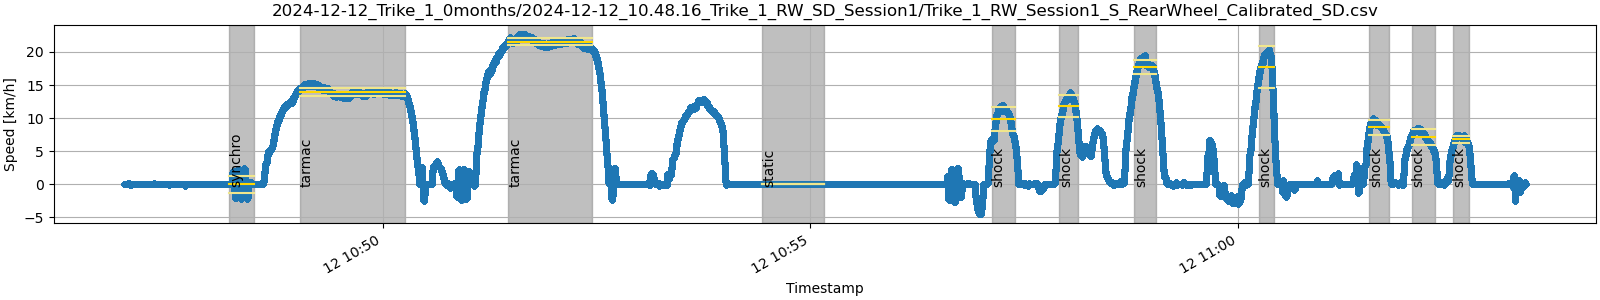
\includegraphics[width=160mm]{fig/session015.png}
  \caption{Vehicle speed versus time derived from the wheel hub IMU for an
  entire session (015) showing the trials in the shaded grey areas. Gold
  horizontal lines depict the mean speed during trials bounded by its standard
  deviation.}
  \label{fig:session}
\end{figure}
%
\begin{enumerate}
  \item Calculate the vehicle travel speed during the session from the angular
    rate of the rear wheel and the vehicle's wheel radius.
  \item Extract segments representing a single trial from each session time
    history, based on the manually labelled segment ``start'', and ``end'' times.
  \item Split the trials with durations longer than 40~\si{\second} into
    repetitions of \SIrange{20}{39}{\second}. Trials less than 20~\si{\second}
    are not split.
  \item Rotate the accelerometer data for each sensor from body-fixed sensor
    coordinates to body-fixed vehicle coordinates. This is achieved by rotating
    the coordinate axes about the sensor's body-fixed axis, which was manually
    aligned with the vehicle's pitch axis. We subtracted the mean measured
    acceleration due to gravity (standard gravity) giving linear acceleration of
    each sensor projected into the vehicle's SAE body-fixed
    axes~\cite{SocietyofAutomotiveEngineers2008}, named: longitudinal $x$,
    lateral $y$, and vertical $z$.
  \item Extract each motion trial segment and select the vehicle body-fixed
    longitudinal, lateral, and vertical component of the seat pan accelerometer.
\end{enumerate}
%
This resulted in acceleration versus time recordings of 154 total repetitions.
The repetitions have durations in the range of \SIrange{20}{40}{\second} (mean:
25~\si{\second}), see Table~\ref{tab:num-trials}.

% NOTE : This table is autogenerated from the data pipeline scripts and pasted
% in. Do not edit manually. I move the units to a second row manually for width
% conservation.
% file: trial-count-data-frame.txt
\begin{table}
  \centering
  \caption{Number of repetitions performed on each road surface and speed along
  with the mean duration and its standard deviation. Tables
  \ref{tab:summary-stroller} and \ref{tab:summary-bicycle} provide metrics for
  repetition sets.}
\begin{tabular}{llcccc}
\toprule
 &  &  & \multicolumn{2}{c}{Repetitions}\\
 &  & Target Speed & Count & Mean Duration & STD Duration \\
Vehicle Type & Road Surface & [\si{\kph}] & & [\si{\second}] & [\si{\second}] \\
\midrule
\multirow[t]{6}{*}{Bicycle} & \multirow[t]{3}{*}{Paver Bricks} & 12 & 13 & 25.1 & 7.0 \\
 &  & 20 & 8 & 28.8 & 7.6 \\
 &  & 25 & 3 & 33.4 & 4.3 \\
\cline{2-6}
 & \multirow[t]{3}{*}{Tarmac} & 12 & 14 & 25.0 & 7.0 \\
 &  & 20 & 6 & 25.2 & 7.2 \\
 &  & 25 & 6 & 22.0 & 2.5 \\
\cline{1-6} \cline{2-6}
\multirow[t]{5}{*}{Stroller} & Cobblestones & 5 & 26 & 22.8 & 5.6 \\
\cline{2-6}
 & Paver Bricks & 5 & 20 & 25.0 & 7.6 \\
\cline{2-6}
 & Sidewalk Pavers & 5 & 19 & 25.2 & 8.2 \\
\cline{2-6}
 & Sidewalk Slabs & 5 & 23 & 22.8 & 3.4 \\
\cline{2-6}
 & Tarmac & 5 & 16 & 28.9 & 9.6 \\
\cline{1-6} \cline{2-6}
 & & \textbf{Count Sum} & \textbf{154} & & \\
\bottomrule
\end{tabular}
  \label{tab:num-trials}
\end{table}

\subsection{Data Analysis}
%
Figure~\ref{fig:vert-acc-example} shows an example time history of the vertical
(\(z\)) acceleration of the seat pan during a single repetition. To perform the
ISO~2631-1 recommended health and comfort analysis, we first downsampled the
time history from the hardware-set variable sampling frequency of approximately
910.22~\si{\hertz} to a constant sample rate of 400~\si{\hertz} using linear
interpolation, giving sufficient samples for the bandwidth of interest based on
the Nyquist frequency. We set any acceleration values outside of the sensor
manufacturer's reported operating range of \(\pm\)16~g to that maximum or
minimum, respectively, given that values outside the range may be unreliable.
Values that exceeded the range only present rarely in nine of the cargo bicycle
paver brick repetitions. Following the ISO~2631-1 recommendation, we low-pass
filtered the signal at \(1.5\times80~\si{\hertz}=120~\si{\hertz}\) using a
zero-lag 2\textsuperscript{nd} order Butterworth filter, given that the standard
only applies to frequencies up to 80~\si{\hertz}.
%
\begin{figure}
  \centering
  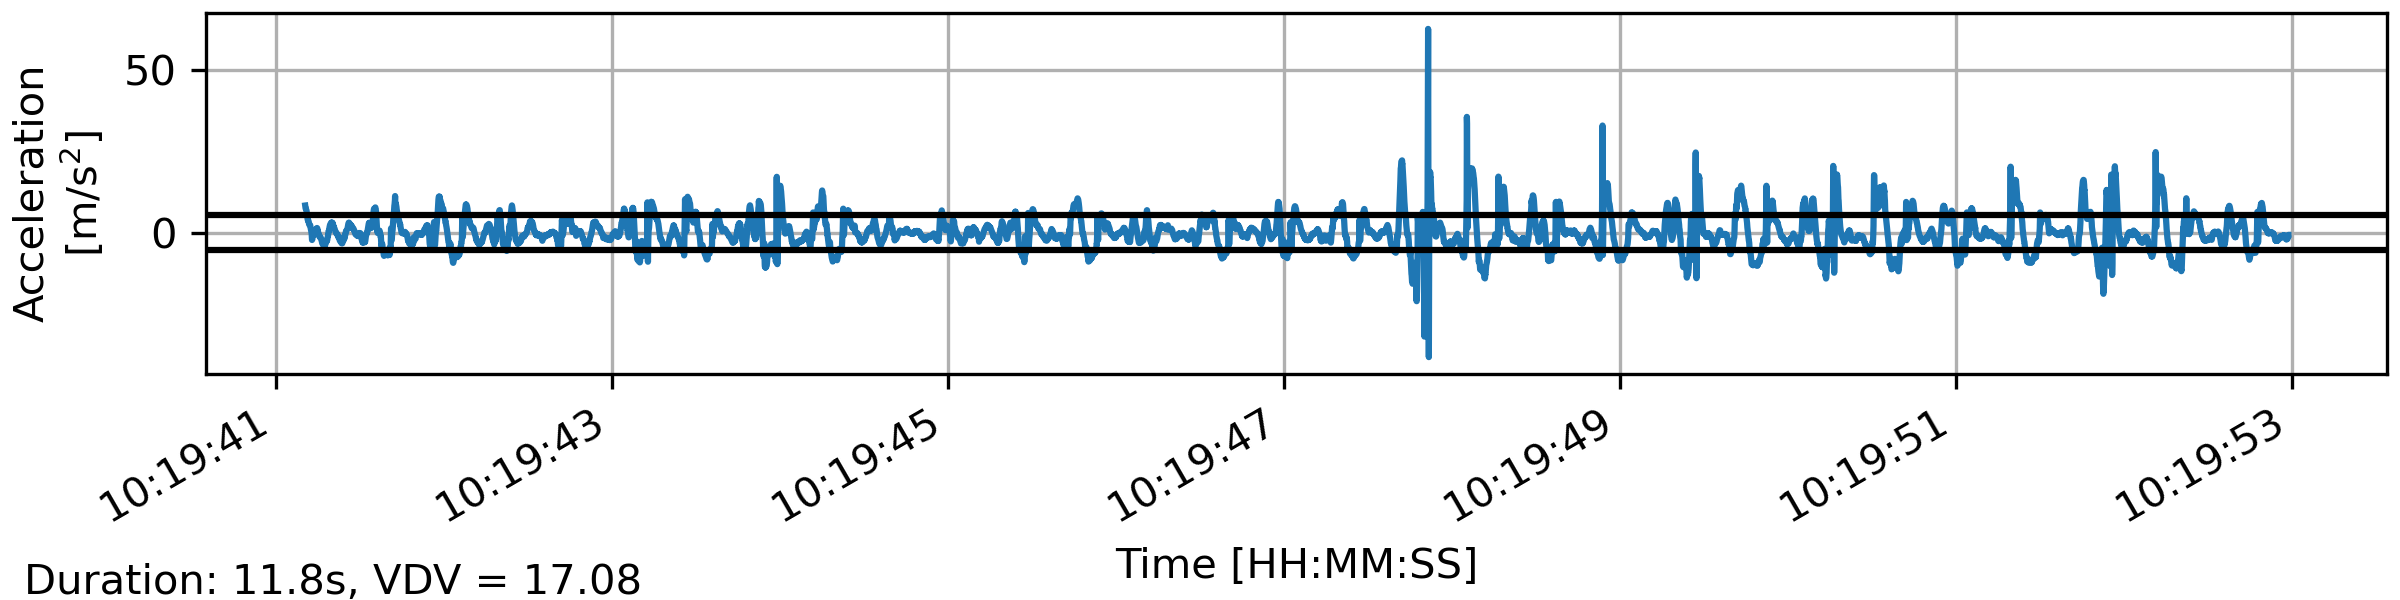
\includegraphics[width=160mm]{fig/session001-t2-aula-stroller-maxicosi-cot-0-SeatBotacc_ver-rep0.png}
  \caption{Raw seat pan vertical acceleration versus time from session 001:
  Maxi-Cosi stroller over the Sidewalk Slabs. Black horizontal lines indicate
  the \(\pm\)root mean square (RMS) about the mean. The vibration dose value
  (VDV) for the first 10~\si{\second} of the printed duration is shown in the
  bottom left.}
  \label{fig:vert-acc-example}
\end{figure}

ISO~2631-1 provides weighting filters that highlight frequencies that adults are
most sensitive to. To apply them, we calculated the amplitude spectra of the
acceleration time histories of each trial using the Fast Fourier Transform
(FFT). Figure~\ref{fig:freq-spectrum} gives an example of a raw amplitude
spectrum along with smoothed versions of the raw and ISO~2631-1 weighted
signals.  In almost all repetitions, there is a single dominant peak frequency
in the ISO weighted and smoothed spectra. A handful of trials had two or more
peaks at adjacent frequencies of approximately the same amplitude. We selected
the maximum amplitude peak in those cases. Before ISO weighting, the area under
the spectrum curve was calculated and the frequency below which 80\% of the
amplitude content falls marked as an indicator of bandwidth.
%
\begin{figure}
  \centering
  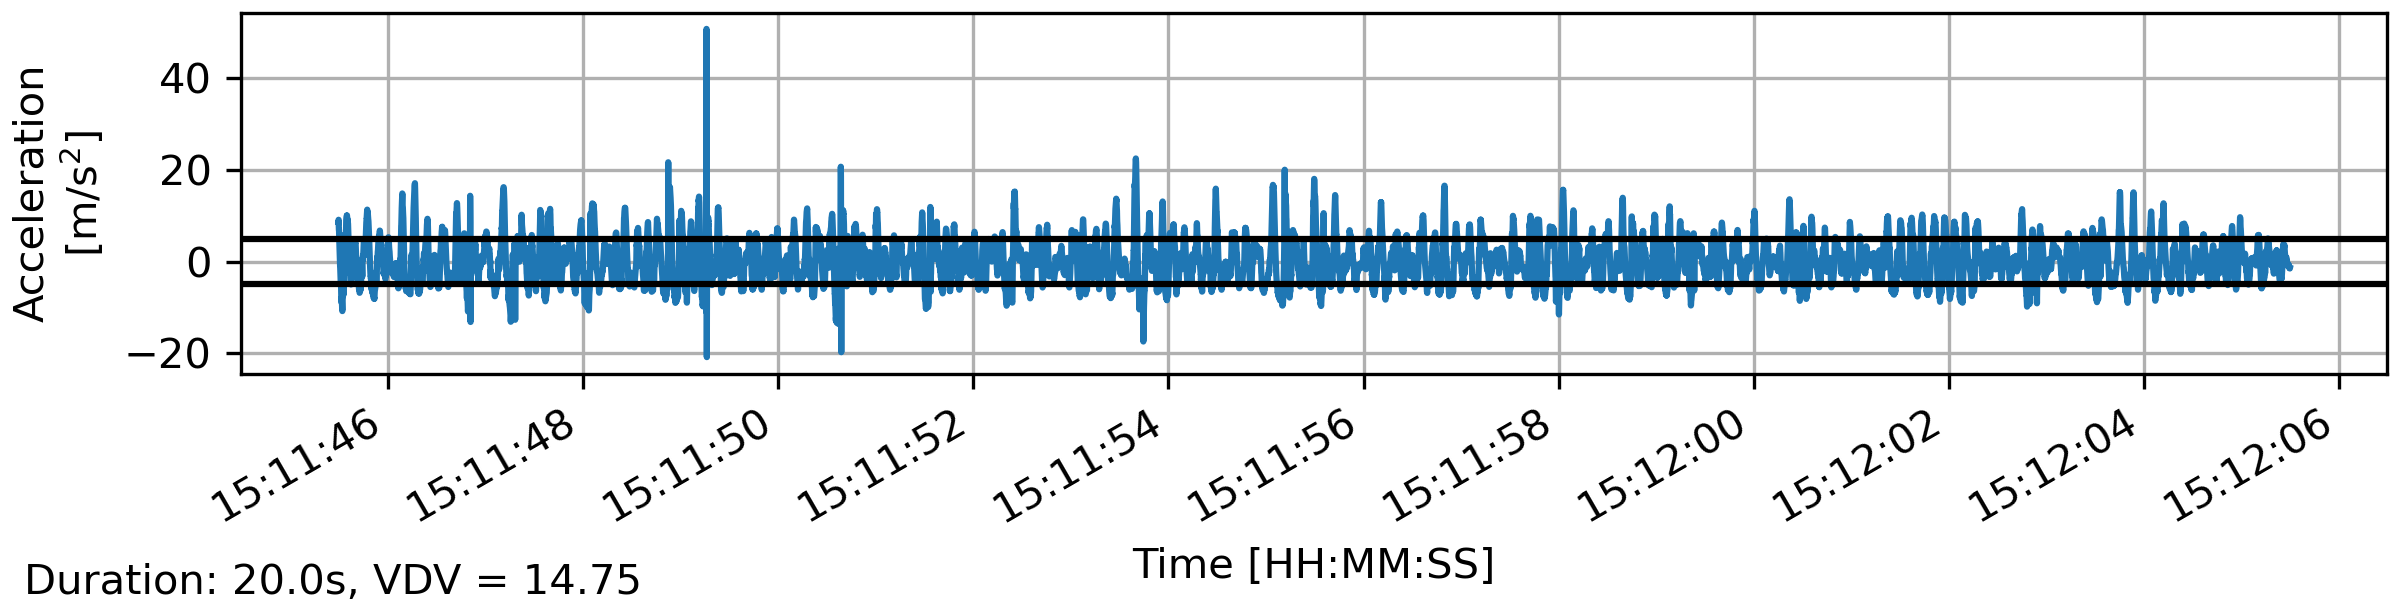
\includegraphics[width=160mm]{fig/session004-t0-pave-stroller-maxicosi-cot-0-SeatBotacc_ver-rep0.png}
  \caption{Seat pan vertical acceleration amplitude spectrum from session 004:
  Maxi-Cosi stroller over cobblestones. The gray curve shows the result of
  the FFT, the black line is a smoothened version of the FFT (zero-lag Butterworth
  low pass), and the blue line is the smoothed ISO weighted FFT. The blue dashed
  vertical line indicates the frequency at the maximum amplitude of the smoothed
  curve. The black dashed-dotted vertical line indicates the bandwidth threshold
  for 80\% of the area under the black curve.}
  \label{fig:freq-spectrum}
\end{figure}

We calculated the root mean square (RMS) over \(N\) samples of the downsampled,
low-pass filtered, and ISO 2631-1 weighted vertical component of acceleration
\(a_{w,z}\) at the seat pan for each repetition using Equation~\ref{eq:rms-acc}
to use for the health assessment and the RMS of the magnitude of the 3D
acceleration vector at the seat pan \(\textrm{RMS}_{a_{w,xyz}}\) using
Equation~\ref{eq:rms-acc-mag} for the comfort assessment, as per ISO 2631-1
guidelines. We set the ISO~2631-1 adjustment factors \(k_x,k_y,k_z\) equal to 1
for all acceleration components. RMS gives an indication of the average vertical
acceleration experienced at the infant's buttocks-seat interface for the
duration of the trial and can be seen in Figure~\ref{fig:vert-acc-example}. It
is the primary metric recommended by ISO-2631-1 for evaluation of health and
comfort in adult whole-body vibration. We also calculated the vibration dose
value \(\textrm{VDV}_{a_{z}}\) of the \(M\) raw data vertical acceleration
\(a_{z}\) samples corresponding to the first 10~\si{\second} of the repetition
with Equation~\ref{eq:vdv-acc}, seen in Figure~\ref{fig:vert-acc-example}.
Lastly, we computed the crest factor \(\textrm{CF}_{a_{z}}\) of the downsampled
and low pass filtered vertical acceleration\footnote{Some scenarios have crest
factors larger than 9, but we do not report metrics other than RMS as ISO~2631-1
recommends for this study.} with Equations~\ref{eq:crest-factor}, respectively.
All of these per-repetition metrics are reported as mean values over the
repetitions corresponding to a scenario in Table~\ref{tab:summary-stroller} and
Table~\ref{tab:summary-bicycle}.
The following
equations describe the metrics:
%
\begin{align}
  \textrm{RMS}_{a_{w,z}} = \sqrt{\frac{1}{N}\sum_{n=1}^{N} k_z^2 a_{w,z}^2(t_n)}
  \label{eq:rms-acc}
\end{align}

\begin{align}
  \textrm{RMS}_{a_{w,xyz}} = \sqrt{\frac{1}{N}\sum_{n=1}^{N} k_x^2 a_{w,x}^2(t_n) + k_y^2 a_{w,y}^2(t_n) + k_z^2 a_{w,z}^2(t_n)}
  \label{eq:rms-acc-mag}
\end{align}

\begin{align}
  \textrm{VDV}_{a_{z}} = \left[\sum_{m=2}^{M} \frac{1}{2} (a_{z,m}^4 - a_{z,m-1}^4) (t_m -t_{m-1})\right]^{1/4}
  \label{eq:vdv-acc}
\end{align}

\begin{align}
  \textrm{CF}_{a_{z}} =\frac{\max|a_{z}(t_m)|}{\sqrt{\frac{1}{M}\sum_{m=1}^{M} a_{z}^2(t_m)}}
  \label{eq:crest-factor}
\end{align}

\subsection{Statistical Modelling}
%
To determine how road surface and stroller setup predict ISO~2631-1 weighted
vertical RMS acceleration, we fitted an ordinary linear least squares model to
the data using:
%
\begin{align}
  \textrm{RMS}_{a_{w,z}} = 
  \beta_0 +
  \beta_1 x_\textrm{Road Surface} +
  \beta_2 x_\textrm{Stroller} +
  \epsilon
\end{align}
%
Both \(x_\textrm{Road Surface}\) and \(x_\textrm{Stroller}\) are categorical
variables, and we selected tarmac and the Green Machine as reference values when
coding the categorical variables, respectively. We did not consider the
interaction of road surface and stroller given no expectation of such an effect.

To determine how speed, road surface, and cargo bicycle setup predict ISO~2631-1
weighted vertical RMS acceleration, we fit an ordinary linear least squares
model to the data using:
%
\begin{align}
  \textrm{RMS}_{a_{w,z}} = 
  \kappa_0 +
  \kappa_1 x_\textrm{Road Surface} +
  \kappa_2 x_\textrm{Cargo Bicycle} + 
  \kappa_3 x_\textrm{Speed} +
  \kappa_4 x_\textrm{Road Surface} \times x_\textrm{Speed} +
  \epsilon
\end{align}
%
Both \(x_\textrm{Road Surface}\) and \(x_\textrm{Cargo Bicycle}\) are
categorical variables and \(x_\textrm{Speed}\) is a continuous variable. We
selected tarmac and the `Keiler, Pebble, 0 mo' setup as the reference values
when coding the categorical variables, respectively. We did not consider the
interaction of road surface and cargo bicycle setup given no expectation of such
an effect but we did consider the interaction of speed with road surface. For
both strollers and cargo bicycles, each tested combination of vehicle, seat, and
dummy size was considered as a different vehicle type. We use \(p<0.05\) to
indicate significant differences for both models. Following fitting of the two
statistical models, we applied Tukey's Range Test to compare vehicle setups
among each other for the different road surfaces and speed ranges with
\(p=0.05\) for the adjusted limit for significance.

\section{Results}
%
Results for all 67 combinations of vehicle setup, road surface, and target speed
are shown in Table~\ref{tab:summary-stroller} for strollers and
Table~\ref{tab:summary-bicycle} for cargo bicycles. These tables show the mean
values over scenario repetitions. They report the unweighted and ISO~2631-1
weighted seat pan vertical RMS acceleration, weighted seat pan magnitude RMS
acceleration, unweighted seat pan vertical VDV for the first 10 seconds of the
repetition, crest factor, peak frequency, bandwidth, and duration for all
combinations of vehicle setup, road surface, and target speed.

The magnitude (combining \(x,y,z\)) ISO weighted RMS is only a bit higher
(\(<\)4\% in  modern strollers and cargo bicycles) than the vertical (\(z\)) ISO
weighted RMS, indicating that vertical vibration is dominant. This also holds
for the Keiler tricycle, which will roll due to differing road unevenness at
left and right wheels, resulting in lateral seat motion, but this seems hardly
relevant in the current data. An exception is the Green Machine where the
magnitude is up to 24\% higher, indicating relevant contributions of horizontal
seat pan motion, which may be due to the lack of rigid horizontal constraint on
the cot. As expected, in all cases the vertical ISO weighted RMS acceleration is
below the vertical unweighted RMS, and this reduction is on average 10\% for
modern strollers, 13\% for the vintage Green Machine, and even 56\% for the
vintage Old Rusty which sees the highest bandwidth (105 Hz). For cargo bicycles,
ISO weighting leads to an average reduction of 16\%. The Keiler with Melia on
paver bricks at 20~\si{\kph} sees a 29\% reduction with a bandwidth of
83~\si{\hertz}. These strong effects of ISO frequency weighting in some vehicle
and speed combinations are addressed further in the discussion. Below we present
ISO weighted results for which guidelines have been published using magnitude
for discomfort and vertical for health. 
%
% NOTE : These tables are generated automatically from the Python scripts. I
% manually edit the header rows to fit on the page width. Save the edits between
% toprule and midrule!
% stroller-summary-data-frame.tex
\bgroup
\setlength\tabcolsep{0.4mm}  % reduces horiztonal padding between columns
\begin{table}[!ht]
  \centering
  \caption{Mean computed metrics of the strollers for all 40 non-shock
  scenarios, using seat pan acceleration.}
  \label{tab:summary-stroller}
  \scriptsize
\begin{tabular}{lllcccccccccc}
\toprule
        &            &         &        & .     &     & ISO      & ISO      & 10~\si{\second}    &        &      &       &       \\
        &            &         & Target & Rep.  & RMS & Weighted & Weighted & VDV & Crest  & Peak & Band- & Dur-  \\
        &            & Road    & Speed  & Count & Acc & RMS Acc  & RMS Mag  & Acc & Factor & Freq & width & ation \\
Vehicle & Seat, Baby & Surface & [\si{\kph}] & & [\si{\mps\squared}] & [\si{\mps\squared}] & [\si{\mps\squared}] & [\si{\meter\second}\(^{-1.75}\)] & & [\si{\hertz}] & [\si{\hertz}]       & [\si{\second}]       \\
\midrule
\multirow[t]{10}{*}{bugaboo} & \multirow[t]{5}{*}{cot, 0 mo} & Cobblestones & 5 & 4 & 4.4 & 4.3 & 4.5 & 11.5 & 6.2 & 6.5 & 20.5 & 20.4 \\
\cline{3-13}
 &  & Paver Bricks & 5 & 3 & 2.6 & 2.4 & 2.5 & 6.1 & 4.1 & 9.5 & 23.4 & 23.3 \\
\cline{3-13}
 &  & Sidewalk Pavers & 5 & 2 & 2.9 & 2.7 & 2.9 & 15.6 & 13.5 & 6.1 & 49.8 & 25.4 \\
\cline{3-13}
 &  & Sidewalk Slabs & 5 & 3 & 4.8 & 4.7 & 4.8 & 12.5 & 6.4 & 5.8 & 30.6 & 20.2 \\
\cline{3-13}
 &  & Tarmac & 5 & 2 & 0.7 & 0.6 & 0.7 & 1.7 & 3.3 & 10.1 & 33.3 & 23.1 \\
\cline{2-13} \cline{3-13}
 & \multirow[t]{5}{*}{seat, 9 mo} & Cobblestones & 5 & 4 & 2.5 & 2.3 & 2.5 & 6.2 & 4.7 & 6.6 & 37.9 & 22.5 \\
\cline{3-13}
 &  & Paver Bricks & 5 & 3 & 2.3 & 1.8 & 1.8 & 5.2 & 3.8 & 9.4 & 43.2 & 22.6 \\
\cline{3-13}
 &  & Sidewalk Pavers & 5 & 3 & 1.7 & 1.4 & 1.6 & 4.5 & 5.5 & 7.7 & 39.5 & 24.7 \\
\cline{3-13}
 &  & Sidewalk Slabs & 5 & 3 & 2.4 & 2.2 & 2.3 & 5.9 & 5.3 & 6.0 & 36.6 & 24.5 \\
\cline{3-13}
 &  & Tarmac & 5 & 2 & 0.6 & 0.4 & 0.5 & 1.6 & 6.5 & 8.4 & 51.2 & 34.6 \\
\cline{1-13} \cline{2-13} \cline{3-13}
\multirow[t]{5}{*}{greenmachine} & \multirow[t]{5}{*}{cot, 0 mo} & Cobblestones & 5 & 3 & 3.2 & 2.9 & 3.4 & 7.2 & 5.3 & 4.1 & 38.1 & 23.7 \\
\cline{3-13}
 &  & Paver Bricks & 5 & 2 & 1.6 & 1.3 & 1.6 & 3.2 & 4.5 & 4.2 & 47.4 & 29.6 \\
\cline{3-13}
 &  & Sidewalk Pavers & 5 & 2 & 2.7 & 2.5 & 2.9 & 7.4 & 6.5 & 4.1 & 41.3 & 28.2 \\
\cline{3-13}
 &  & Sidewalk Slabs & 5 & 3 & 3.5 & 3.2 & 3.4 & 7.6 & 6.7 & 3.9 & 36.0 & 23.9 \\
\cline{3-13}
 &  & Tarmac & 5 & 2 & 0.5 & 0.4 & 0.7 & 1.1 & 4.1 & 4.2 & 52.5 & 22.1 \\
\cline{1-13} \cline{2-13} \cline{3-13}
\multirow[t]{10}{*}{maxicosi} & \multirow[t]{5}{*}{cot, 0 mo} & Cobblestones & 5 & 4 & 4.6 & 4.4 & 4.5 & 11.3 & 4.9 & 8.1 & 51.2 & 20.7 \\
\cline{3-13}
 &  & Paver Bricks & 5 & 2 & 3.2 & 2.8 & 2.9 & 7.5 & 3.9 & 10.4 & 53.6 & 27.2 \\
\cline{3-13}
 &  & Sidewalk Pavers & 5 & 3 & 3.0 & 2.9 & 3.0 & 8.3 & 5.5 & 7.6 & 40.1 & 21.4 \\
\cline{3-13}
 &  & Sidewalk Slabs & 5 & 3 & 5.0 & 4.6 & 4.7 & 13.8 & 8.2 & 5.1 & 70.3 & 16.3 \\
\cline{3-13}
 &  & Tarmac & 5 & 2 & 0.9 & 0.8 & 0.8 & 2.1 & 8.0 & 9.6 & 43.4 & 34.3 \\
\cline{2-13} \cline{3-13}
 & \multirow[t]{5}{*}{seat, 9 mo} & Cobblestones & 5 & 3 & 4.1 & 3.7 & 3.8 & 10.4 & 5.8 & 8.0 & 46.9 & 25.9 \\
\cline{3-13}
 &  & Paver Bricks & 5 & 2 & 3.0 & 2.4 & 2.4 & 6.9 & 3.4 & 9.7 & 57.4 & 27.8 \\
\cline{3-13}
 &  & Sidewalk Pavers & 5 & 2 & 2.6 & 2.3 & 2.5 & 7.2 & 5.5 & 7.3 & 47.2 & 27.8 \\
\cline{3-13}
 &  & Sidewalk Slabs & 5 & 3 & 3.1 & 2.9 & 3.0 & 7.8 & 5.4 & 6.9 & 51.4 & 25.6 \\
\cline{3-13}
 &  & Tarmac & 5 & 2 & 1.0 & 0.7 & 0.8 & 2.6 & 5.8 & 10.2 & 55.5 & 36.1 \\
\cline{1-13} \cline{2-13} \cline{3-13}
\multirow[t]{5}{*}{oldrusty} & \multirow[t]{5}{*}{seat, 9 mo} & Cobblestones & 5 & 2 & 4.7 & 2.0 & 2.3 & 13.0 & 6.0 & 5.1 & 105.1 & 29.9 \\
\cline{3-13}
 &  & Paver Bricks & 5 & 3 & 3.4 & 1.2 & 1.4 & 8.7 & 6.1 & 5.2 & 106.1 & 21.9 \\
\cline{3-13}
 &  & Sidewalk Pavers & 5 & 2 & 3.3 & 1.4 & 1.7 & 9.7 & 9.7 & 5.4 & 104.2 & 27.3 \\
\cline{3-13}
 &  & Sidewalk Slabs & 5 & 3 & 3.2 & 1.6 & 1.7 & 10.5 & 11.6 & 5.3 & 103.9 & 23.8 \\
\cline{3-13}
 &  & Tarmac & 5 & 2 & 1.1 & 0.5 & 0.6 & 2.7 & 5.7 & 7.0 & 105.5 & 22.6 \\
\cline{1-13} \cline{2-13} \cline{3-13}
\multirow[t]{10}{*}{stokke} & \multirow[t]{5}{*}{cot, 0 mo} & Cobblestones & 5 & 3 & 4.1 & 4.0 & 4.1 & 10.5 & 4.8 & 6.4 & 66.3 & 21.3 \\
\cline{3-13}
 &  & Paver Bricks & 5 & 2 & 3.0 & 2.1 & 2.2 & 6.9 & 4.1 & 9.4 & 97.7 & 29.5 \\
\cline{3-13}
 &  & Sidewalk Pavers & 5 & 3 & 2.8 & 2.6 & 2.7 & 7.0 & 5.5 & 6.7 & 69.9 & 22.2 \\
\cline{3-13}
 &  & Sidewalk Slabs & 5 & 2 & 4.0 & 3.8 & 3.9 & 11.6 & 6.4 & 5.2 & 79.1 & 25.7 \\
\cline{3-13}
 &  & Tarmac & 5 & 2 & 0.9 & 0.6 & 0.6 & 2.8 & 7.4 & 7.7 & 89.3 & 19.5 \\
\cline{2-13} \cline{3-13}
 & \multirow[t]{5}{*}{seat, 9 mo} & Cobblestones & 5 & 3 & 5.2 & 4.9 & 5.0 & 12.4 & 4.4 & 7.7 & 69.1 & 21.5 \\
\cline{3-13}
 &  & Paver Bricks & 5 & 3 & 3.6 & 3.0 & 3.0 & 8.2 & 3.8 & 10.4 & 93.4 & 22.5 \\
\cline{3-13}
 &  & Sidewalk Pavers & 5 & 2 & 3.1 & 2.7 & 2.8 & 11.9 & 9.9 & 8.3 & 78.3 & 28.5 \\
\cline{3-13}
 &  & Sidewalk Slabs & 5 & 3 & 4.0 & 3.7 & 3.8 & 9.7 & 6.2 & 5.3 & 69.7 & 23.3 \\
\cline{3-13}
 &  & Tarmac & 5 & 2 & 0.7 & 0.4 & 0.5 & 1.9 & 6.3 & 11.1 & 95.6 & 39.1 \\
\cline{1-13} \cline{2-13} \cline{3-13}
\bottomrule
\end{tabular}
\end{table}
\egroup

% bicycle-summary-data-frame.tex
\bgroup
\setlength\tabcolsep{0.4mm}  % reduces horiztonal padding between columns
\begin{table}[!ht]
  \centering
  \caption{Mean computed metrics of the cargo bicycles for all 27 non-shock scenarios, using seat pan
  acceleration.}
  \label{tab:summary-bicycle}
  \scriptsize
\begin{tabular}{lllcccccccccc}
\toprule
        &            &         &        & .     &     & ISO      & ISO      & 10~\si{\second}    &        &      &       &       \\
        &            &         & Target & Rep.  & RMS & Weighted & Weighted & VDV & Crest  & Peak & Band- & Dur-  \\
        &            & Road    & Speed  & Count & Acc & RMS Acc  & RMS Mag  & Acc & Factor & Freq & width & ation \\
Vehicle & Seat, Baby & Surface & [\si{\kph}] & & [\si{\mps\squared}] & [\si{\mps\squared}] & [\si{\mps\squared}] & [\si{\meter\second}\(^{-1.75}\)] & & [\si{\hertz}] & [\si{\hertz}]       & [\si{\second}]       \\
\midrule
\multirow[t]{12}{*}{keiler} & \multirow[t]{4}{*}{melia, 3 mo} & \multirow[t]{2}{*}{Paver Bricks} & 12 & 2 & 5.4 & 4.9 & 5.0 & 12.9 & 8.1 & 7.9 & 62.5 & 26.3 \\
 &  &  & 20 & 2 & 9.5 & 6.7 & 6.9 & 31.9 & 10.2 & 6.8 & 82.6 & 23.0 \\
\cline{3-13}
 &  & \multirow[t]{2}{*}{Tarmac} & 12 & 2 & 1.2 & 1.2 & 1.3 & 2.7 & 8.2 & 7.8 & 41.6 & 25.4 \\
 &  &  & 20 & 2 & 1.6 & 1.5 & 1.6 & 3.6 & 3.8 & 8.3 & 28.9 & 22.6 \\
\cline{2-13} \cline{3-13}
 & \multirow[t]{4}{*}{pebble, 0 mo} & \multirow[t]{2}{*}{Paver Bricks} & 12 & 2 & 7.0 & 6.9 & 7.1 & 15.7 & 7.2 & 7.6 & 36.6 & 23.8 \\
 &  &  & 20 & 1 & 12.6 & 10.7 & 10.9 & 26.6 & 9.9 & 6.8 & 74.8 & 34.0 \\
\cline{3-13}
 &  & \multirow[t]{2}{*}{Tarmac} & 12 & 3 & 1.8 & 1.8 & 1.9 & 6.4 & 8.3 & 8.1 & 18.7 & 24.6 \\
 &  &  & 20 & 2 & 2.8 & 2.8 & 2.8 & 6.7 & 5.1 & 7.8 & 16.7 & 29.2 \\
\cline{2-13} \cline{3-13}
 & \multirow[t]{4}{*}{pebble, 3 mo} & \multirow[t]{2}{*}{Paver Bricks} & 12 & 2 & 6.3 & 5.7 & 5.9 & 14.7 & 11.0 & 8.0 & 47.5 & 28.9 \\
 &  &  & 20 & 2 & 9.8 & 7.8 & 8.0 & 28.7 & 14.4 & 7.2 & 68.3 & 21.4 \\
\cline{3-13}
 &  & \multirow[t]{2}{*}{Tarmac} & 12 & 2 & 1.5 & 1.5 & 1.6 & 4.9 & 8.1 & 7.6 & 18.5 & 27.8 \\
 &  &  & 20 & 2 & 2.1 & 2.1 & 2.2 & 5.1 & 3.9 & 6.4 & 16.0 & 23.8 \\
\cline{1-13} \cline{2-13} \cline{3-13}
\multirow[t]{15}{*}{urbanarrow} & \multirow[t]{5}{*}{melia, 3 mo} & \multirow[t]{3}{*}{Paver Bricks} & 12 & 2 & 4.5 & 4.1 & 4.1 & 12.0 & 8.3 & 7.5 & 31.9 & 24.1 \\
 &  &  & 20 & 1 & 6.9 & 6.2 & 6.3 & 15.2 & 8.6 & 7.9 & 40.1 & 36.8 \\
 &  &  & 25 & 1 & 7.6 & 6.8 & 6.8 & 15.1 & 7.2 & 9.2 & 47.7 & 31.7 \\
\cline{3-13}
 &  & \multirow[t]{2}{*}{Tarmac} & 12 & 3 & 0.9 & 0.9 & 0.9 & 3.6 & 9.3 & 9.4 & 33.2 & 20.4 \\
 &  &  & 25 & 2 & 1.4 & 1.3 & 1.3 & 3.4 & 5.8 & 9.4 & 27.8 & 23.0 \\
\cline{2-13} \cline{3-13}
 & \multirow[t]{5}{*}{pebble, 0 mo} & \multirow[t]{3}{*}{Paver Bricks} & 12 & 3 & 6.5 & 5.7 & 5.7 & 26.1 & 9.6 & 7.6 & 58.5 & 20.8 \\
 &  &  & 20 & 1 & 9.2 & 8.5 & 8.6 & 15.5 & 9.9 & 8.0 & 53.1 & 39.1 \\
 &  &  & 25 & 1 & 11.6 & 8.2 & 8.3 & 31.8 & 13.7 & 6.9 & 85.0 & 38.3 \\
\cline{3-13}
 &  & \multirow[t]{2}{*}{Tarmac} & 12 & 2 & 1.3 & 1.2 & 1.2 & 4.8 & 8.3 & 9.3 & 24.8 & 29.0 \\
 &  &  & 25 & 2 & 2.1 & 1.9 & 1.9 & 4.7 & 5.2 & 9.7 & 24.6 & 21.5 \\
\cline{2-13} \cline{3-13}
 & \multirow[t]{5}{*}{pebble, 3 mo} & \multirow[t]{3}{*}{Paver Bricks} & 12 & 2 & 4.5 & 3.9 & 3.9 & 11.5 & 13.5 & 5.8 & 46.0 & 29.1 \\
 &  &  & 20 & 1 & 10.8 & 7.4 & 7.5 & 15.2 & 14.7 & 5.0 & 71.9 & 32.1 \\
 &  &  & 25 & 1 & 10.6 & 7.7 & 7.8 & 36.3 & 14.7 & 6.3 & 71.0 & 30.3 \\
\cline{3-13}
 &  & \multirow[t]{2}{*}{Tarmac} & 12 & 2 & 1.1 & 1.0 & 1.0 & 3.8 & 9.6 & 8.8 & 28.3 & 25.3 \\
 &  &  & 25 & 2 & 1.6 & 1.5 & 1.5 & 3.8 & 4.9 & 9.5 & 25.4 & 21.6 \\
\cline{1-13} \cline{2-13} \cline{3-13}
\bottomrule
\end{tabular}
\end{table}
\egroup

\subsection{Effect of Speed and model with Cargo Bicycles}
%
Figure~\ref{fig:bicycle-type-compare} compares the two cargo bicycle models
which were both fitted with the same set of two baby seats (Melia and Pebble).
Keiler sees higher accelerations compared to the two-wheeled Urban Arrow, with a
pronounced increase on tarmac and a modest increase on paver bricks. Both
vehicles show increasing accelerations with speed.
%
\begin{figure}
  \centering
  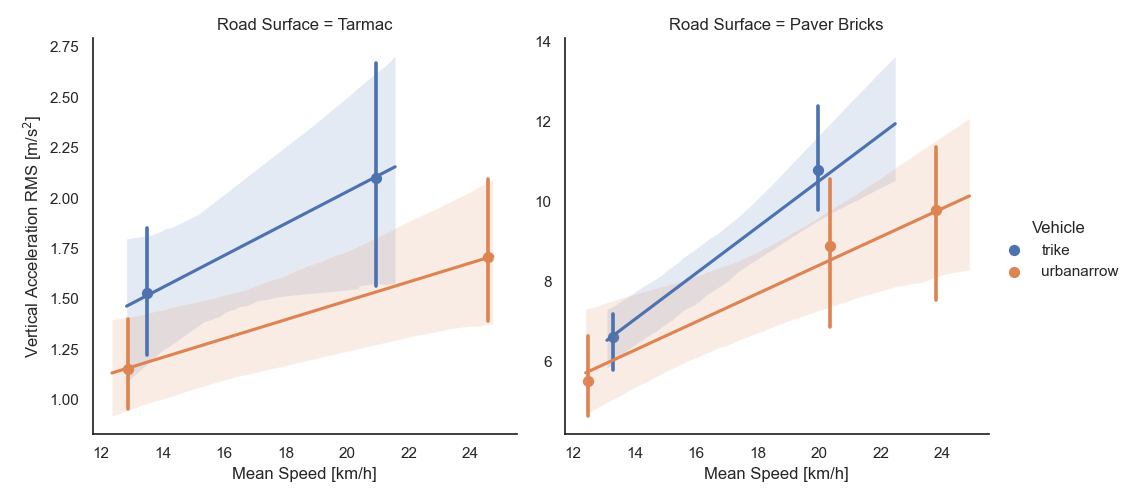
\includegraphics[width=160mm]{fig/SeatBotacc_ver-bicycle-type-compare.png}
  \caption{Seat pan ISO~2631-1 weighted vertical RMS acceleration versus speed
  grouped by road surface and cargo bicycle model. Slanted lines indicate a
  linear regression, vertical lines are the standard deviation at those speeds,
  and shaded regions show the 95\% confidence intervals for the regression.}
  \label{fig:bicycle-type-compare}
\end{figure}

\subsection{Effect of Stroller Model}
%
Figure~\ref{fig:stroller-type-compare} shows the vertical RMS accelerations for
each road surface for each of the five strollers, lumping seat configurations
and dummy sizes. The Maxi-Cosi and Stokke strollers have similar mean values.
The Bugaboo has a slightly lower mean for cobblestones, paver bricks, and
sidewalk pavers. The Green Machine performs better than the modern strollers on
paver bricks, but similarly otherwise. The Old Rusty performs better than the
modern strollers on all surfaces except tarmac. All strollers seem to experience
similar accelerations on tarmac. All road surfaces compared to tarmac at least
double the RMS acceleration.
%
\begin{figure}
  \centering
  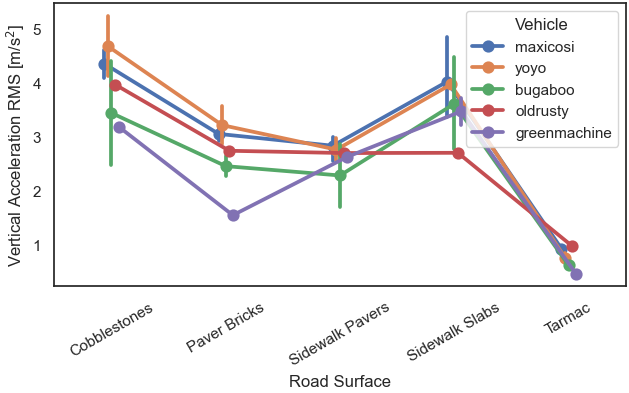
\includegraphics[width=160mm]{fig/SeatBotacc_ver-stroller-type-compare.png}
  \caption{Seat pan ISO 2631-1 weighted vertical RMS acceleration per road
  surface for each stroller. Vertical lines indicate the standard deviation for
  categories that have more than one repetition.} 
  \label{fig:stroller-type-compare}
\end{figure}

\subsection{Dominant Frequency and Bandwidth}
%
Figure~\ref{fig:spectra-compare} shows frequency spectra averaged over body size
and posture for all strollers on sidewalk pavers (left) and cargo bicycles on
paver bricks. These surfaces are highly relevant as they are common in the
Netherlands. Apparently, the two vintage strollers show a lower peak frequency,
which is 4.1~\si{\hertz} for Green Machine and 5.6~\si{\hertz} for Old Rusty
whereas modern systems peak around \SIrange{7}{9}{\hertz}. This can be explained
by the more compliant suspension of the vintage strollers. The Old Rusty shows
the lowest acceleration peak, and the lowest RMS weighted acceleration, but
above 30 Hz it shows the highest power of all strollers. The Keiler sees much
higher peak values as compared to the Urban Arrow. In both cargo bicycles, the
peak frequencies range from \SIrange{6}{10}{\hertz} and hardly depend on vehicle
and speed. Figure~\ref{fig:peak-freq-dist} shows the distributions of the
dominant (peak) frequency across road surface types for each of the target
speeds. Peak frequencies range from about \SIrange{4}{11}{\hertz} across all
trials. For strollers (5~\si{\kph}), the median frequency increases from
sidewalk slabs to cobblestones and sidewalk pavers and then to tarmac and paver
bricks. For cargo bicycles, the difference in peak frequency between the two
road surfaces is not as apparent or consistent.
%
\begin{figure}
  \centering
  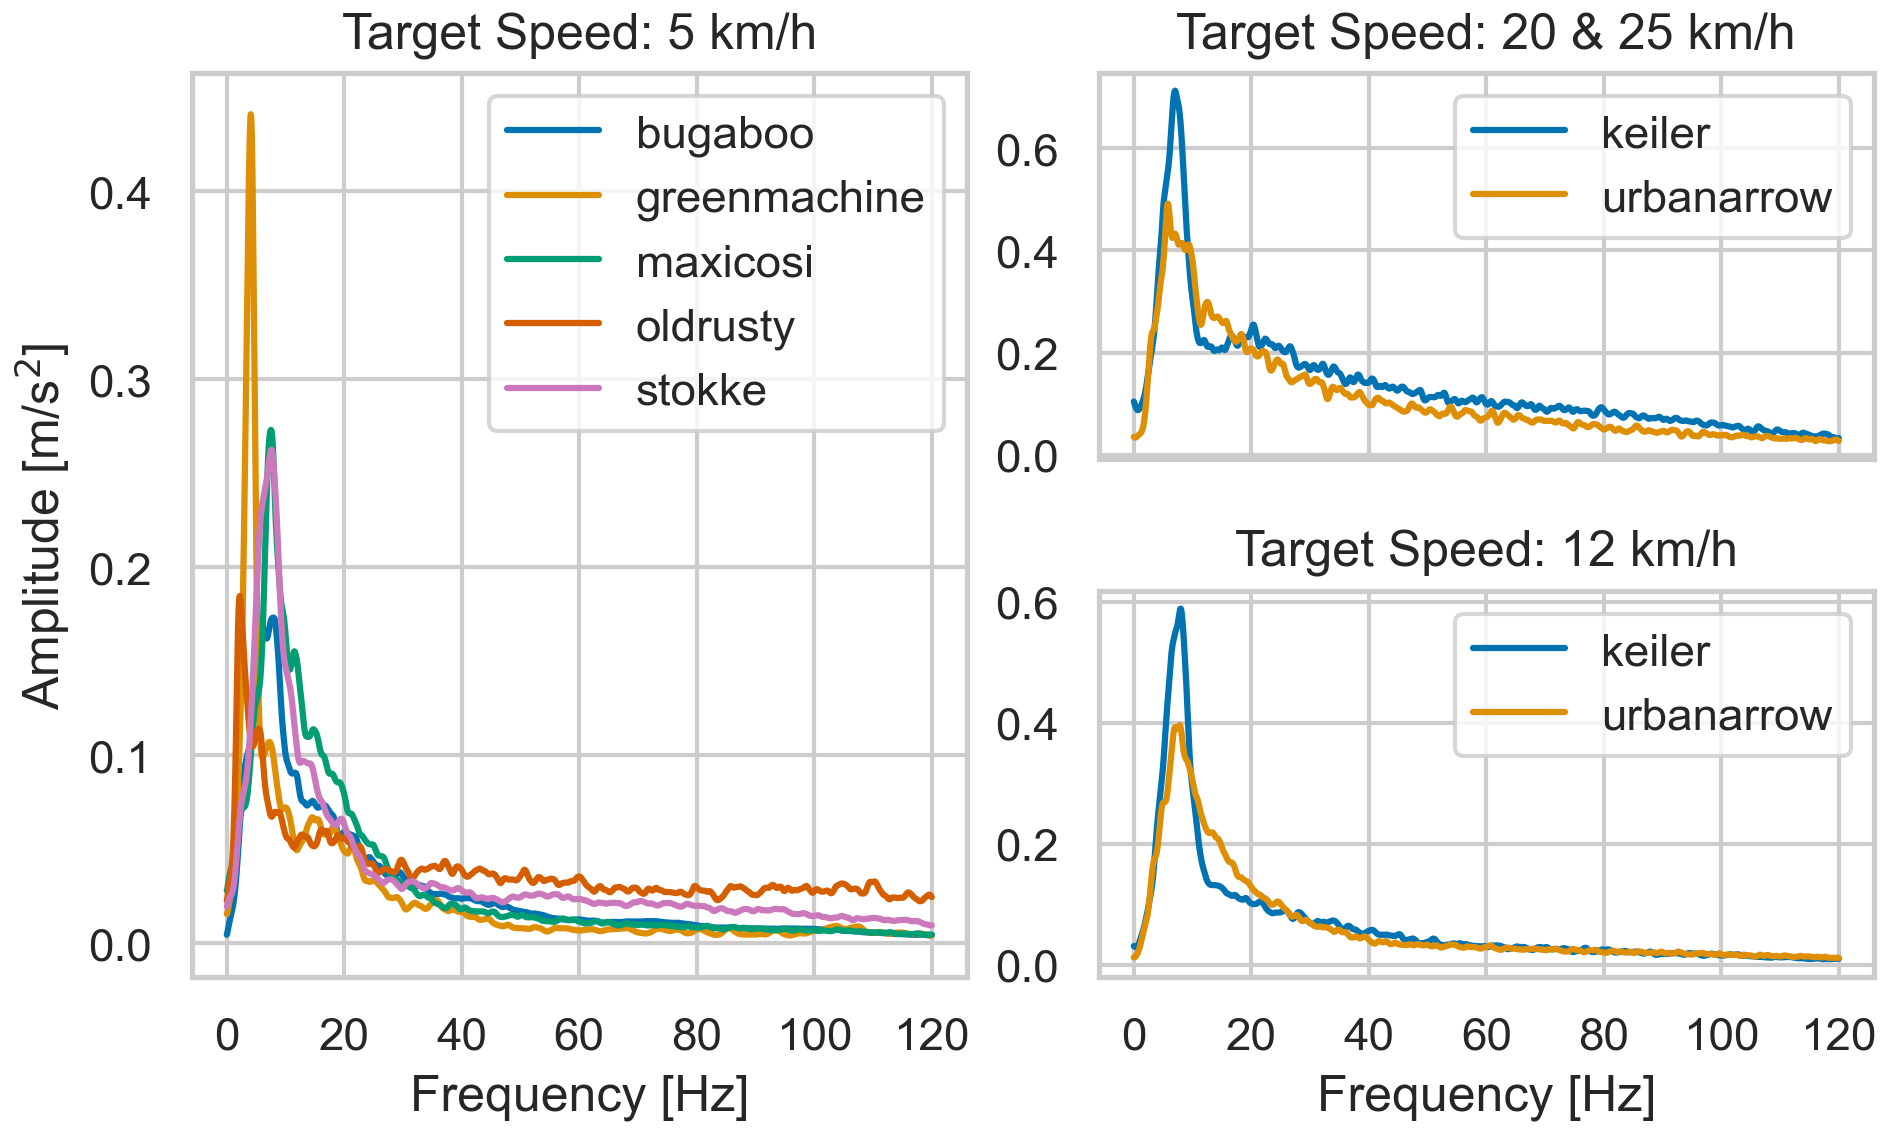
\includegraphics[width=160mm]{fig/SeatBotacc_ver-spectra-compare.png}
  \caption{Mean vertical seat pan amplitude spectra of each vehicle for
  strollers on sidewalk pavers (left) and cargo bicycles on paver bricks
  (right).} 
  \label{fig:spectra-compare}
\end{figure}
%
\begin{figure}
  \centering
  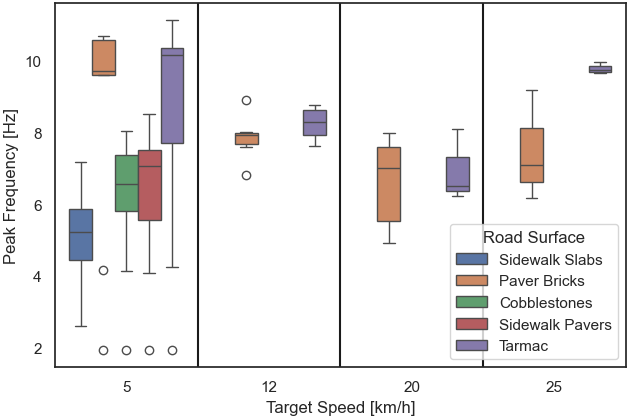
\includegraphics[width=160mm]{fig/SeatBotacc_ver-peak-freq-dist.png}
  \caption{Seat pan vertical peak frequency distributions comparisons among road surfaces for each
  target speed group for non-shock repetitions. The boxes bound the quartiles
  and indicate the median. The whiskers indicate the 95\textsuperscript{th}
  percentile and circles are outliers.}
  \label{fig:peak-freq-dist}
\end{figure}

Figure~\ref{fig:bandwidth-dist} gives a general indication of the bandwidth (80\% of
the amplitude spectrum content) for each of the target speed groups. On average,
the bandwidth is 56 Hz for modern strollers, 46 Hz for Green Machine, 105 Hz for
Old Rusty, and 44 Hz for cargo bicycles.
%
\begin{figure}
  \centering
  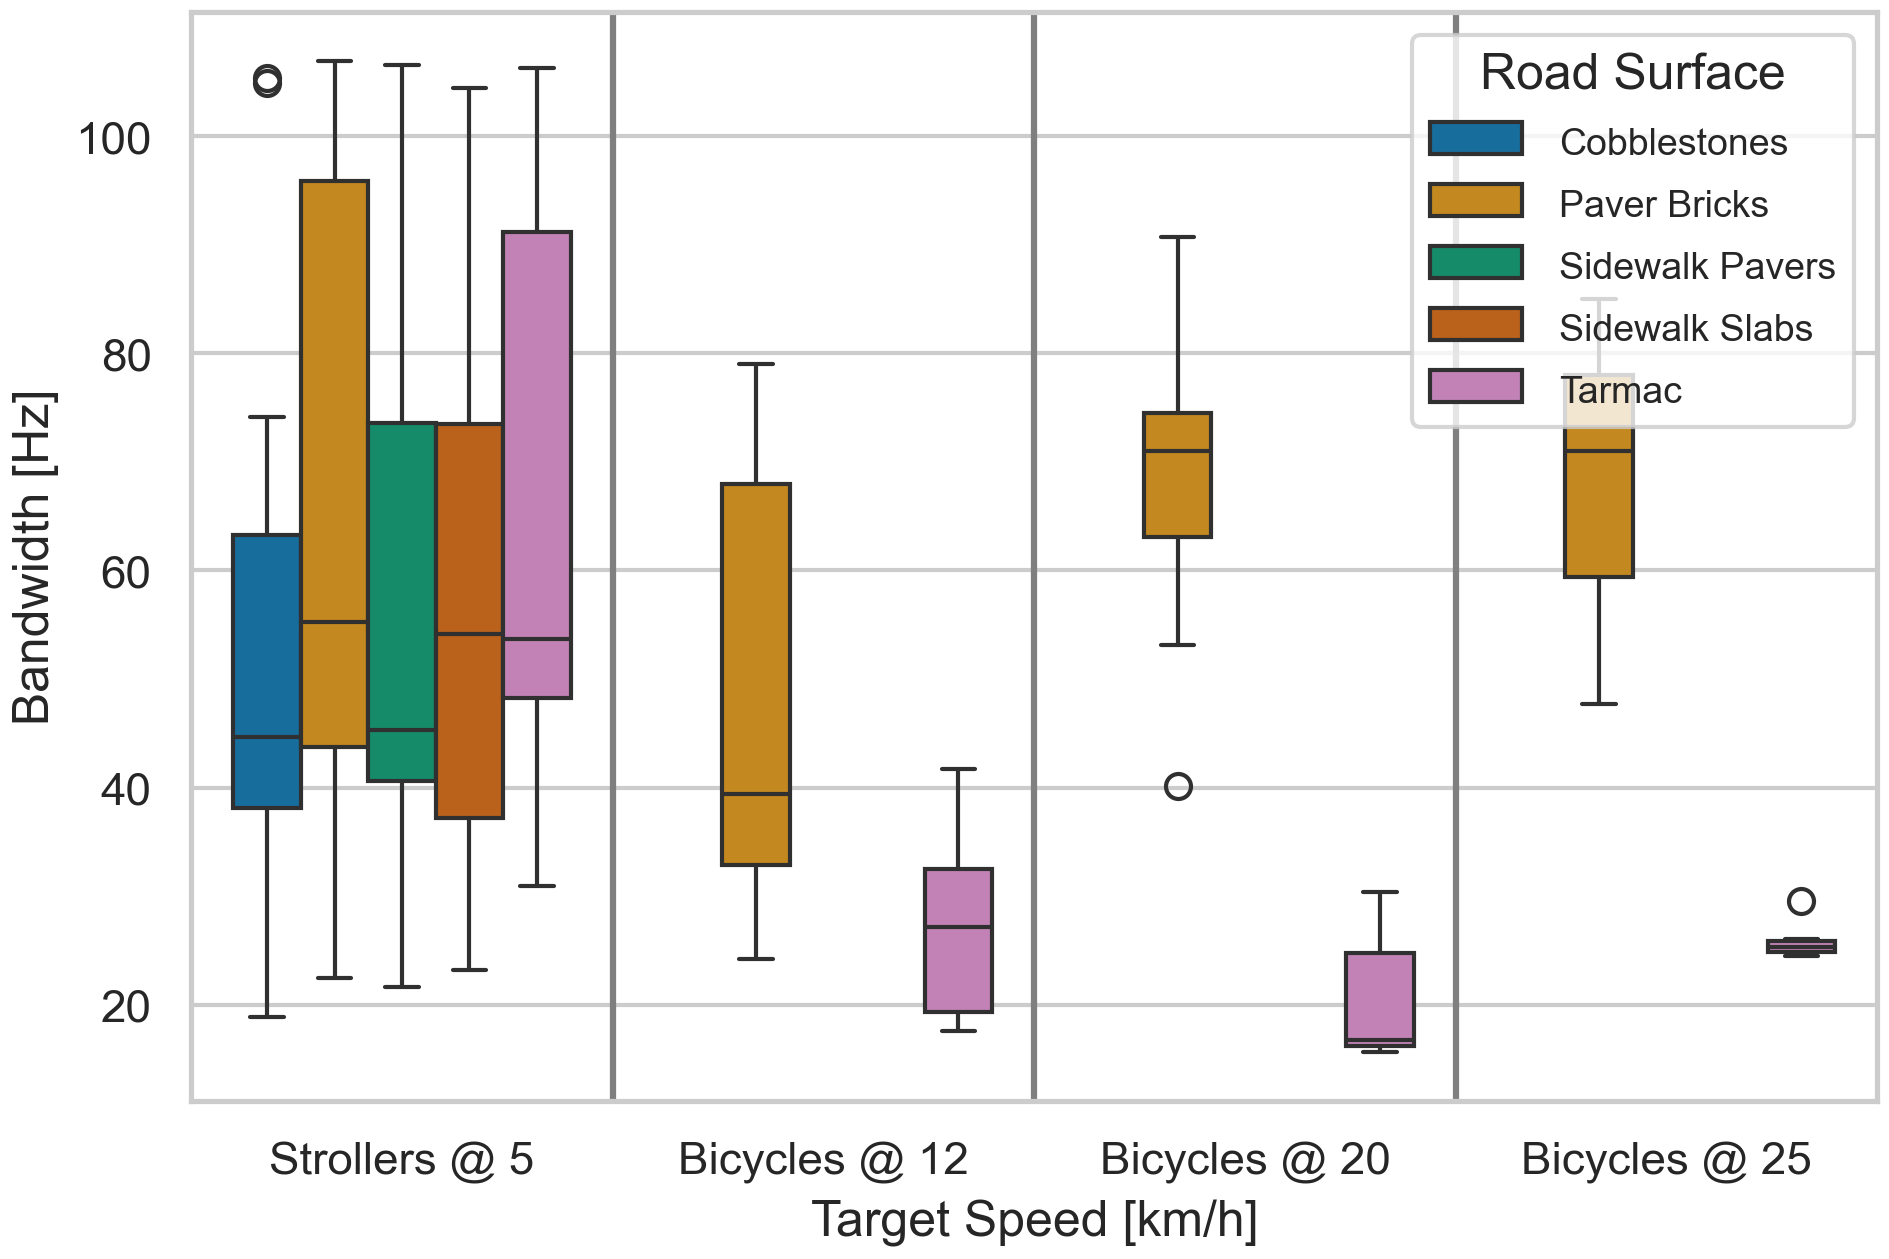
\includegraphics[width=160mm]{fig/SeatBotacc_ver-bandwidth-dist.png}
  \caption{Bandwidth (based on 80\% of the area under the unfiltered seat pan
  vertical amplitude spectrum) for each target speed group for non-shock
  repetitions. The boxes bound the quartiles and indicate the median. The
  whiskers indicate the 95\textsuperscript{th} percentile and circles are
  outliers.}
  \label{fig:bandwidth-dist}
\end{figure}

\subsection{Health Assessment}
\label{sec:health-assesment}
%
Figures \ref{fig:health-stroller} and \ref{fig:health-bicycle} show the
ISO~2631-1 weighted vertical acceleration at the seat pan for all repetitions of
the stroller and cargo bicycles, respectively. The horizontal lines in the
figure correspond to the boundaries of the ``health caution'' and  ``health
risk'' zones in the standard, which depend on the duration of exposure. If
acceleration values are above the health caution zone, ISO~2631-1 states that
``health risks are likely'' for adults in erect seating postures for a
continuous daily dose. It must be emphasised that ISO~2631-1 is based on adults
and may not result in a representative risk for infants or older children.
%
\begin{figure}
  \centering
  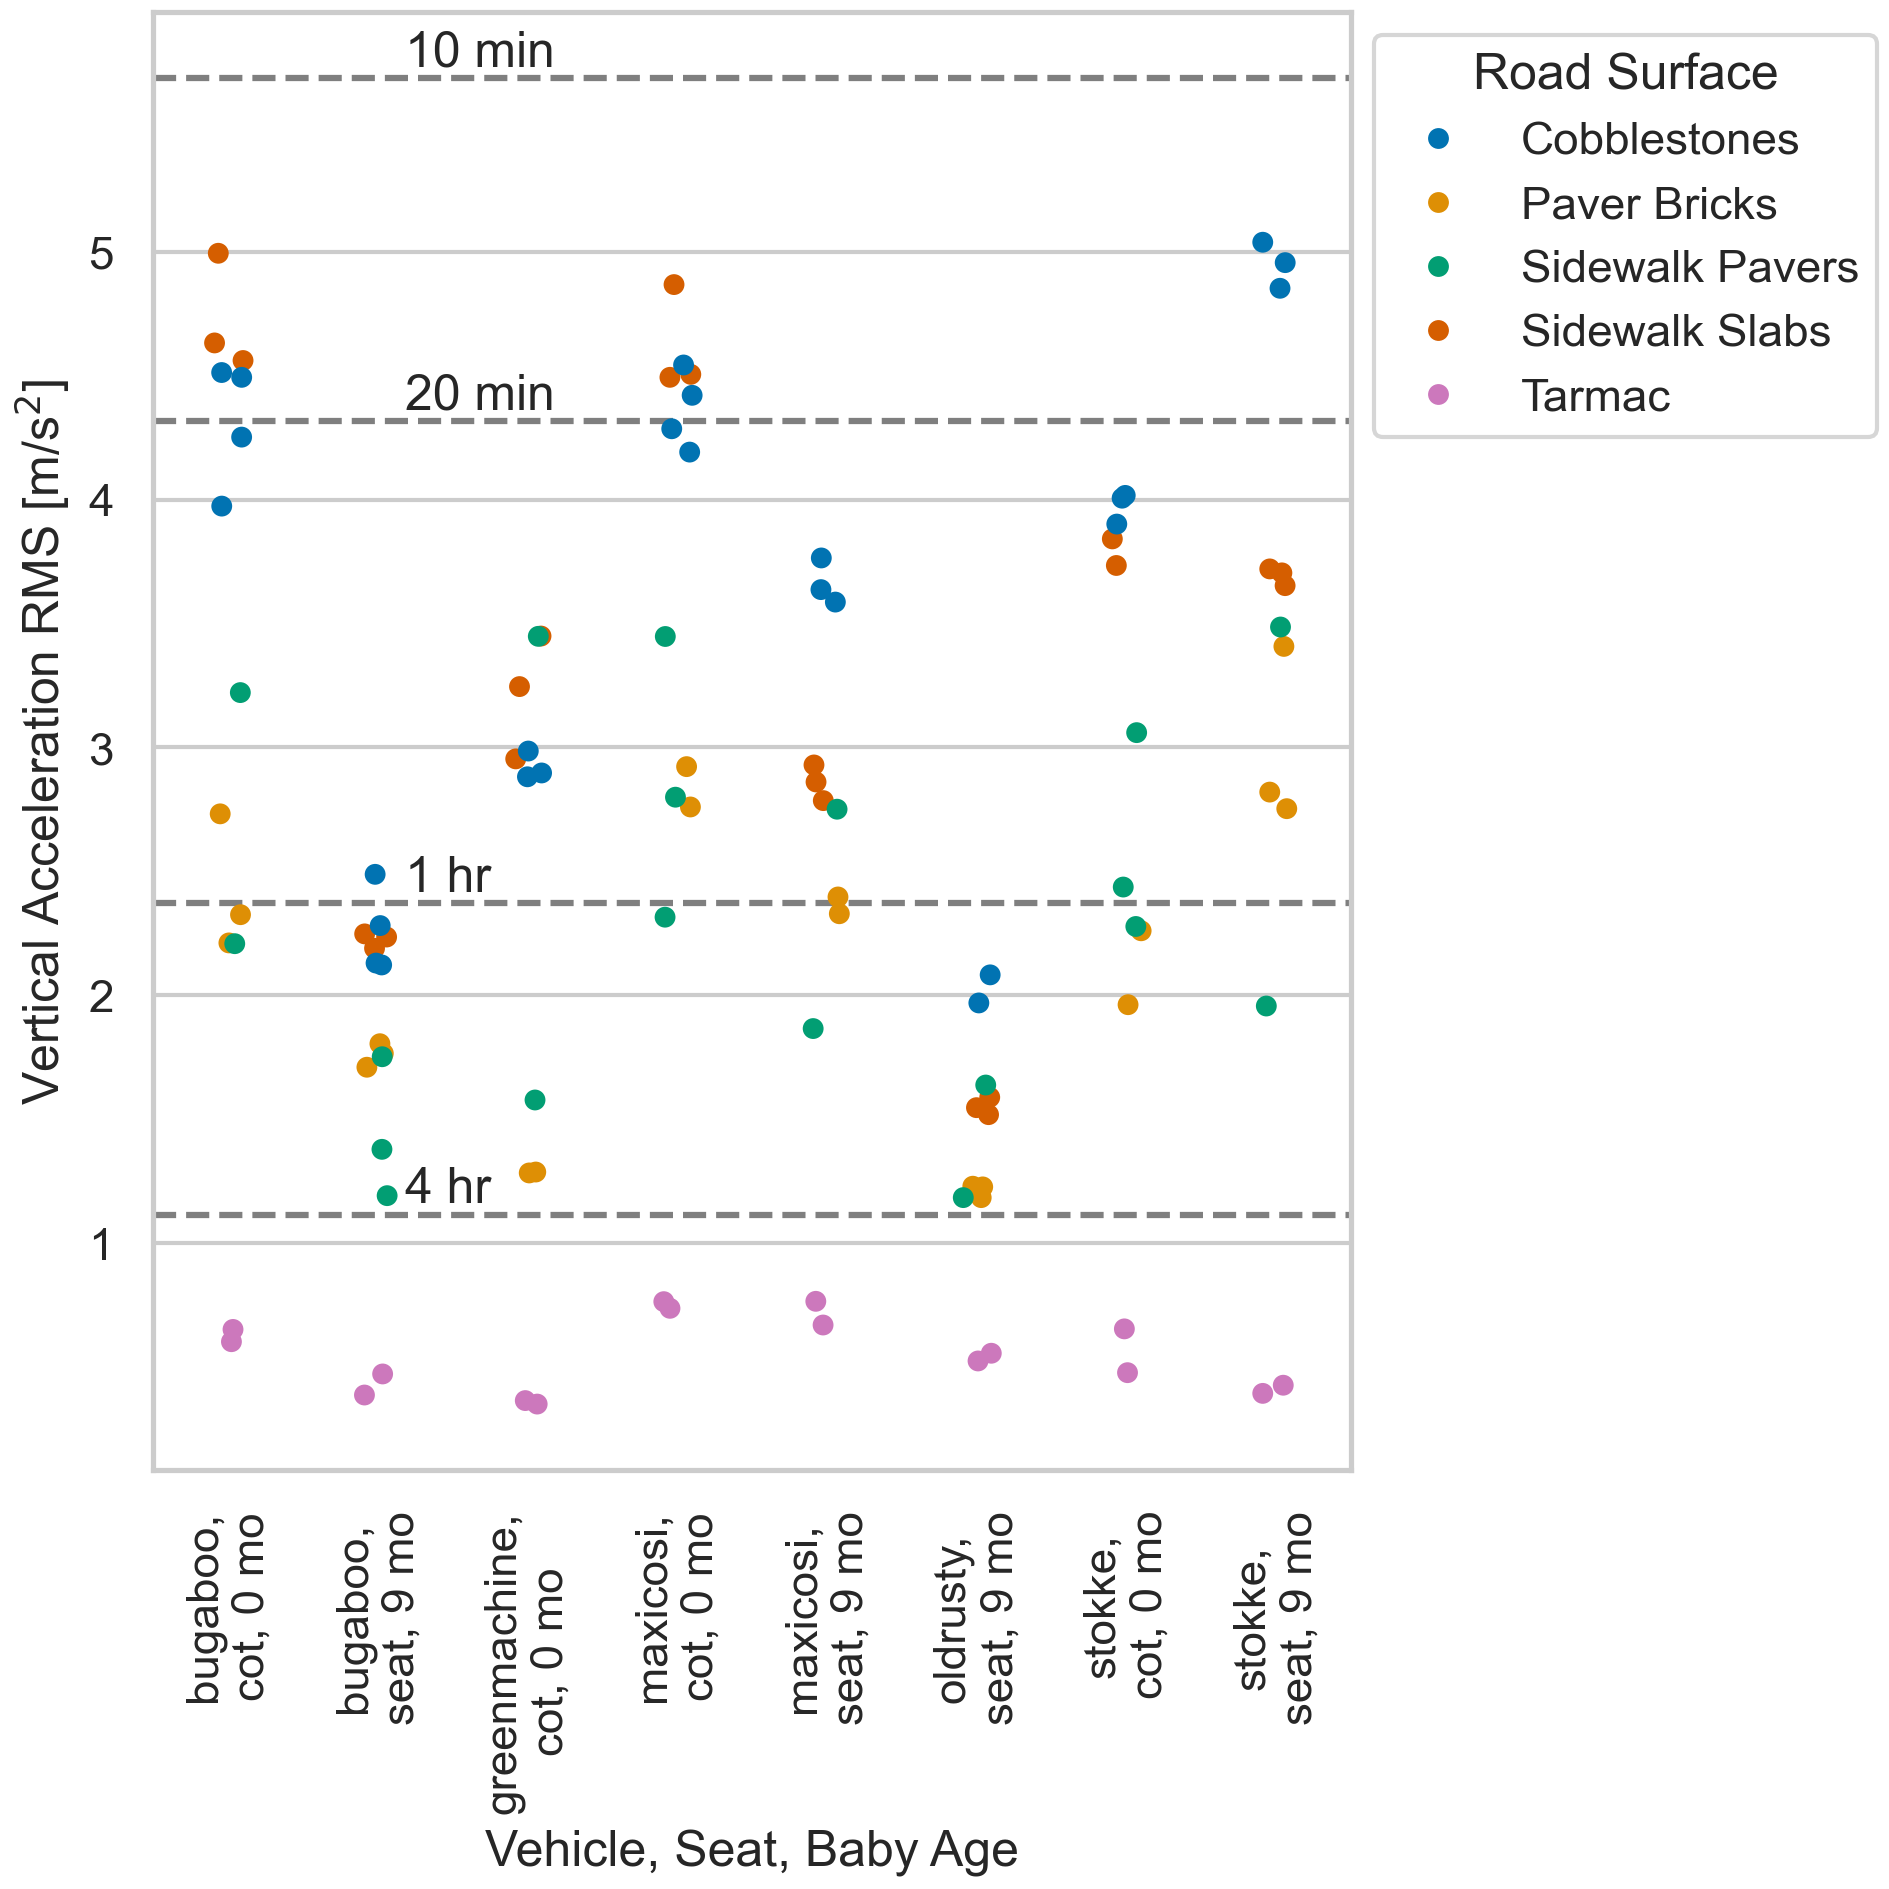
\includegraphics[width=160mm]{fig/SeatBotacc_ver-rms-stroller-compare-all.png}
  \caption{ISO~2631-1 weighted seat pan vertical RMS acceleration of all
  stroller repetitions with colour representing road surface. The horizontal
  dashed grey lines with time duration indicators are the upper bounds of the
  ISO~2631-1 ``health caution zones'' for long-term exposure of adults seated
  erectly, daily experiencing these vibrations with continuous duration.}
  \label{fig:health-stroller}
\end{figure}
%
\begin{figure}
  \centering
  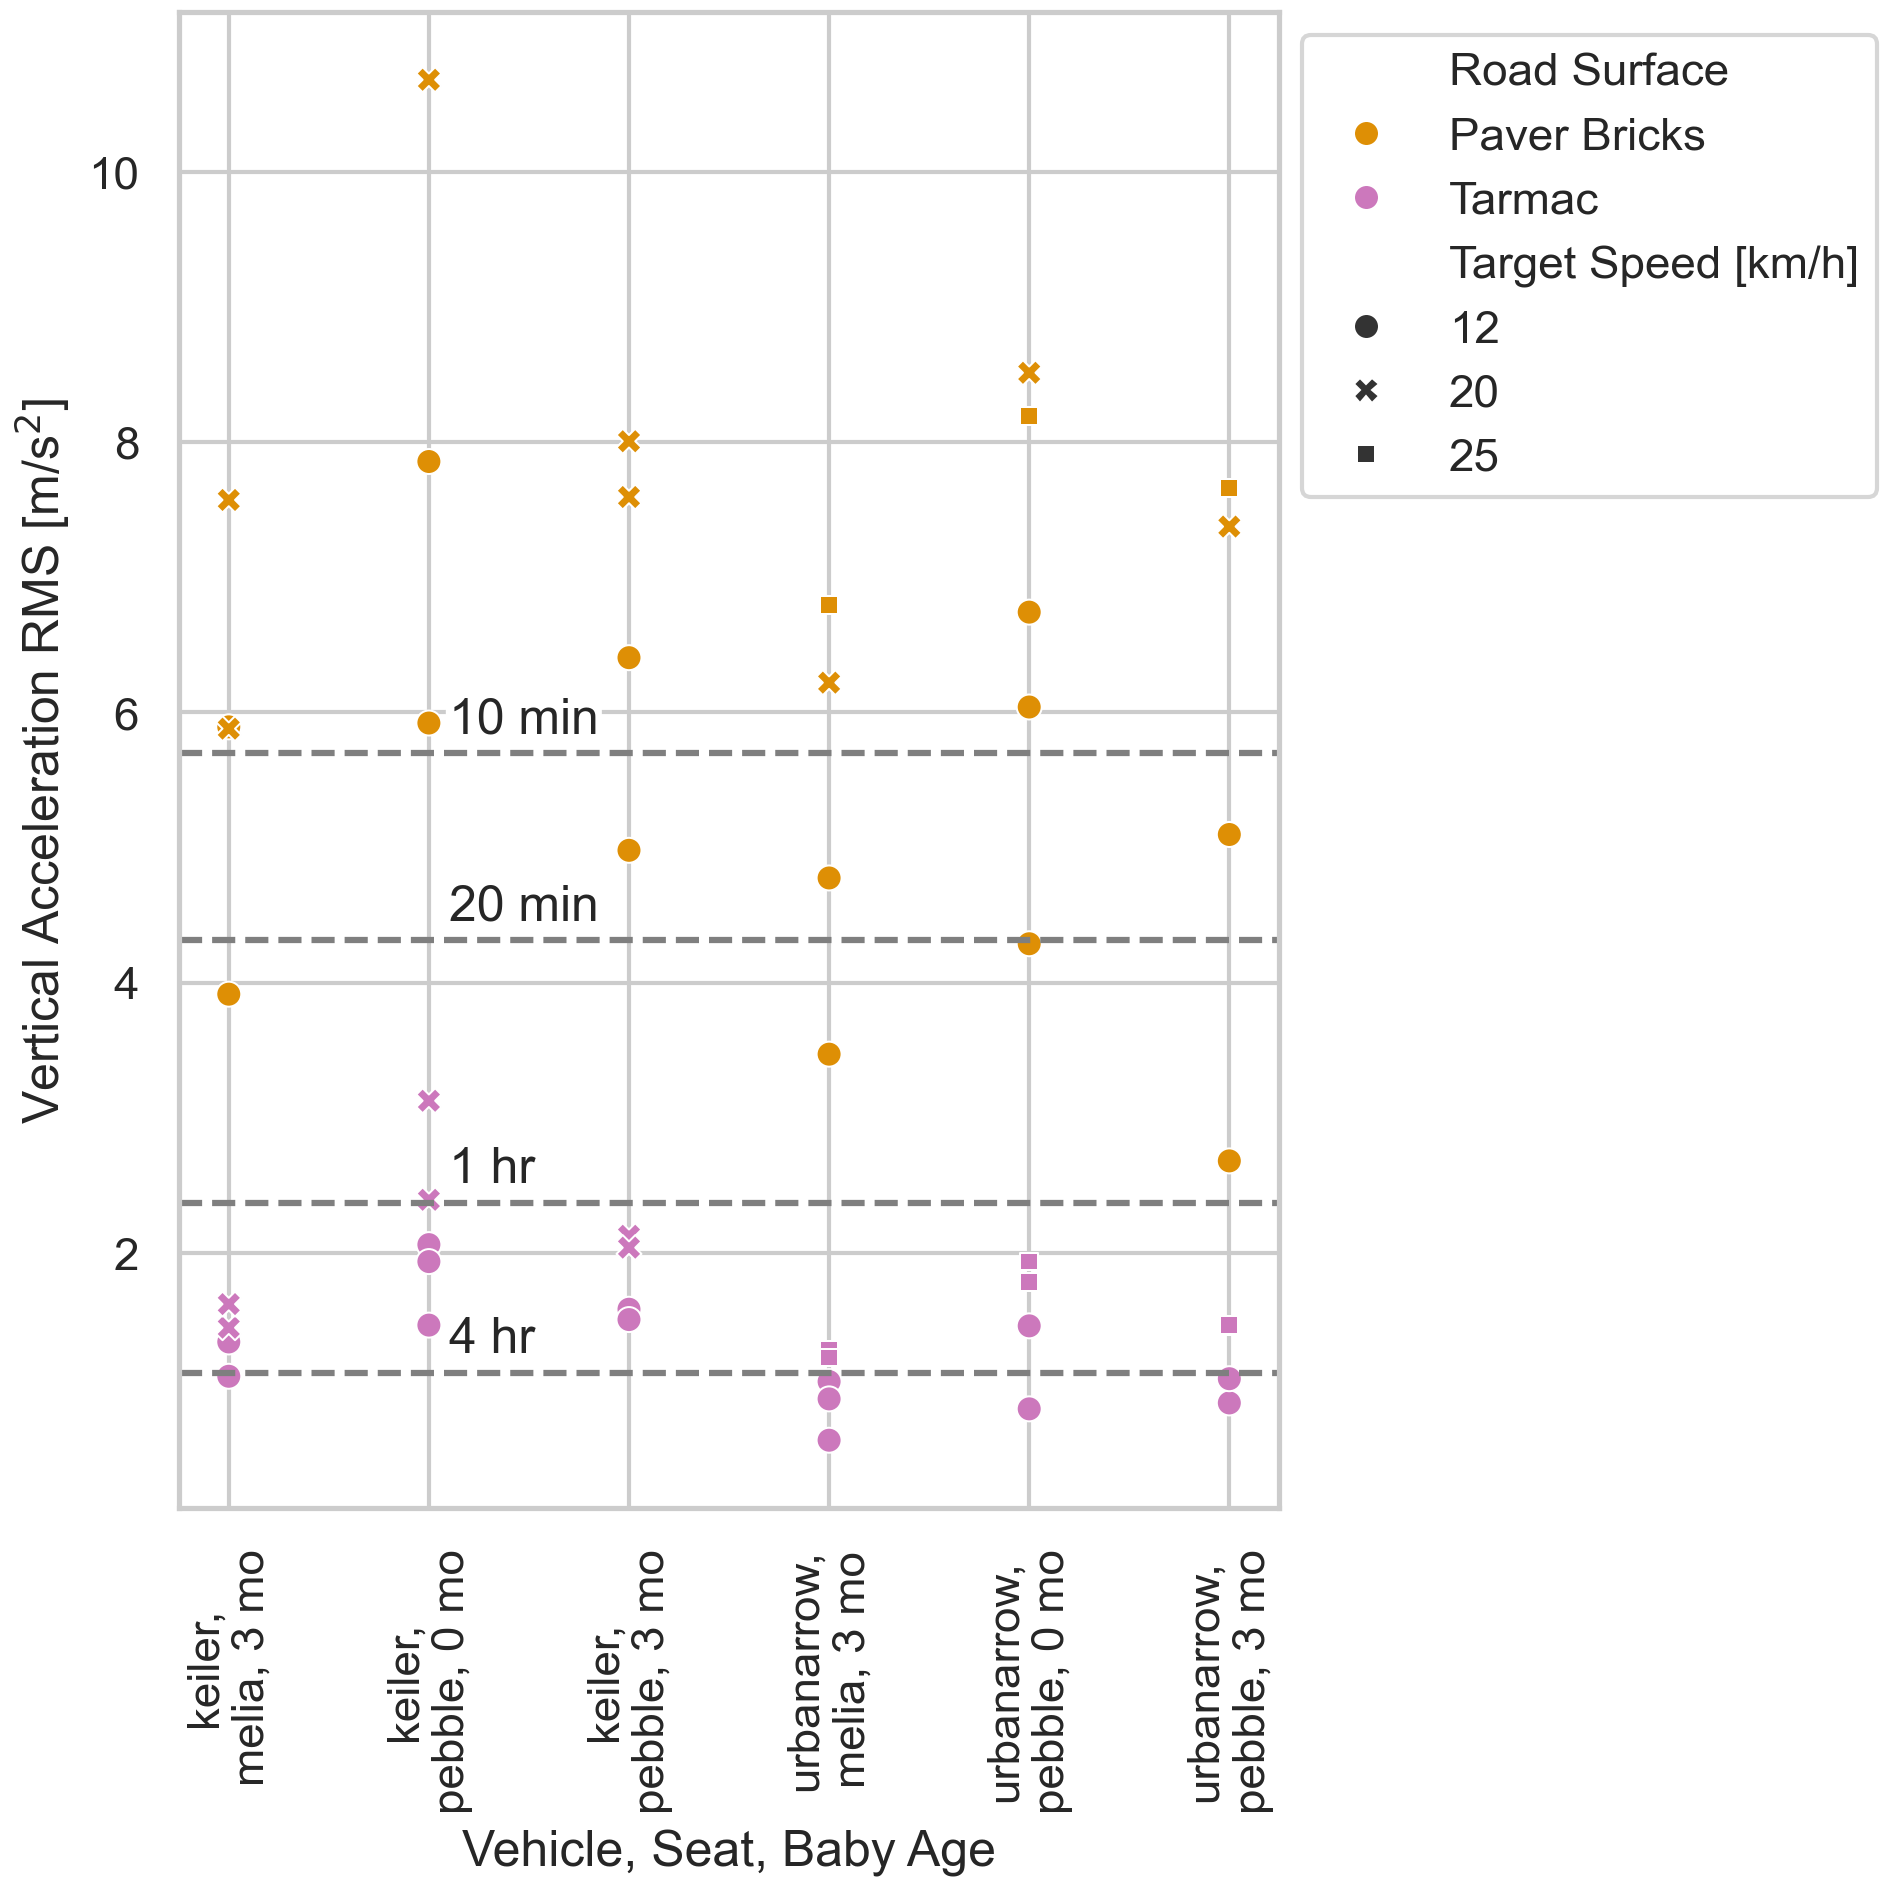
\includegraphics[width=160mm]{fig/SeatBotacc_ver-rms-bicycle-compare-all.png}
  \caption{ISO~2631-1 weighted seat pan vertical RMS acceleration of all cargo
  bicycle trials with colour representing road surface and marker style
  indicating the target speed. The horizontal dashed grey lines with time
  duration indicators are the upper bounds of the ISO~2631-1 ``health caution
  zones'' for long-term exposure of adults seated erectly, daily experiencing
  these vibrations with continuous duration.}
  \label{fig:health-bicycle}
\end{figure}

For the strollers, all vibration measurements were below the health caution zone
boundary if the long-term daily continuous exposure is under 10~\si{\minute}.
Additionally, all strollers pushed over tarmac were below the zone for long-term
daily continuous exposure under 4~\si{\hour}. Pushing the Bugaboo and Maxi-Cosi
with a 0-month-old infant or the Stokke with a 9-month-old infant over
cobblestones and sidewalk slabs may have health risks for long-term daily
continuous exposures exceeding 20~\si{\minute}. For almost all strollers,
pushing over any surface except tarmac exceeded the 1~\si{\hour} risk boundary.
Notably the Bugaboo and Old Rusty with a 9-month-old infant fell at or under the
1~\si{\hour} threshold for all surfaces. The 0-month dummy experienced worse
accelerations than the 9-month dummy in the Bugaboo and Maxi-Cosi, but that was
opposite for the Stokke. Old Rusty showed the lowest overall acceleration
magnitudes.

For both cargo bicycles, accelerations exceeded the 10~\si{\minute} health risk
threshold when ridden above 20~\si{\kilo\meter\per\hour} on paver bricks and
exceeded the health risk threshold when ridden more than 1~\si{\hour} above
12~\si{\kilo\meter\per\hour} on paver bricks. All but the Keiler with the Pebble
and the 0-month dummy were below the 1~\si{\hour} threshold for riding on tarmac
at any target speed. Only the Urban Arrow with the 3-month dummy was (mostly)
under the 4~\si{\hour} threshold when ridden at either speed over tarmac. The
accelerations were lower for the Melia versus the Pebble, which is statistically
confirmed in Section~\ref{sec:statistical-results}.

\subsection{Comfort Assessment}
%
ISO~2631-1 recommends using the magnitude of the weighted seat pan acceleration
3D vector for comfort assessment. Figures \ref{fig:comfort-stroller} and
\ref{fig:comfort-bicycle} plot RMS of the acceleration magnitude along with the
comfort indicators provided in the standard that are based on adults seated in
public transit for an unspecified duration. It must be emphasised that the
ISO~2631-1 comfort assessment was compiled for adults, with many warnings and
limitations, and may not be applicable for other contexts or populations, like
infants or older children. We also include a line representing cyclists'
discomfort threshold reported by Gao~et.~al~\cite{Gao2018}. It is important to
recognise that cyclists perched on a bicycle seat seem to tolerate higher
vibration amplitudes than the public transit riders who were surveyed for the
ISO ratings. This points to possible weakness in or contradiction to the ISO
recommendations or to other factors affecting cycling discomfort (e.g., the
ability to stand on the pedals to lower vibration to the body and the head).

When following the threshold definitions from the ISO~2631-1 guidelines for the
strollers, all are at least ``a little uncomfortable'' on all surfaces. All
strollers but the Stokke are ``fairly uncomfortable'' on tarmac. All other road
surfaces are at least ``very uncomfortable''. The `Bugaboo, seat, 9 mo' and
`Green Machine, cot, 0 mo' over paver bricks and `Old Rusty, seat, 9 mo' over
paver bricks, sidewalk pavers, and sidewalk slabs are ``very uncomfortable'',
but all other strollers and surfaces are ``extremely uncomfortable''. The Old
Rusty generally shows the lowest discomfort levels.
%
\begin{figure}
  \centering
  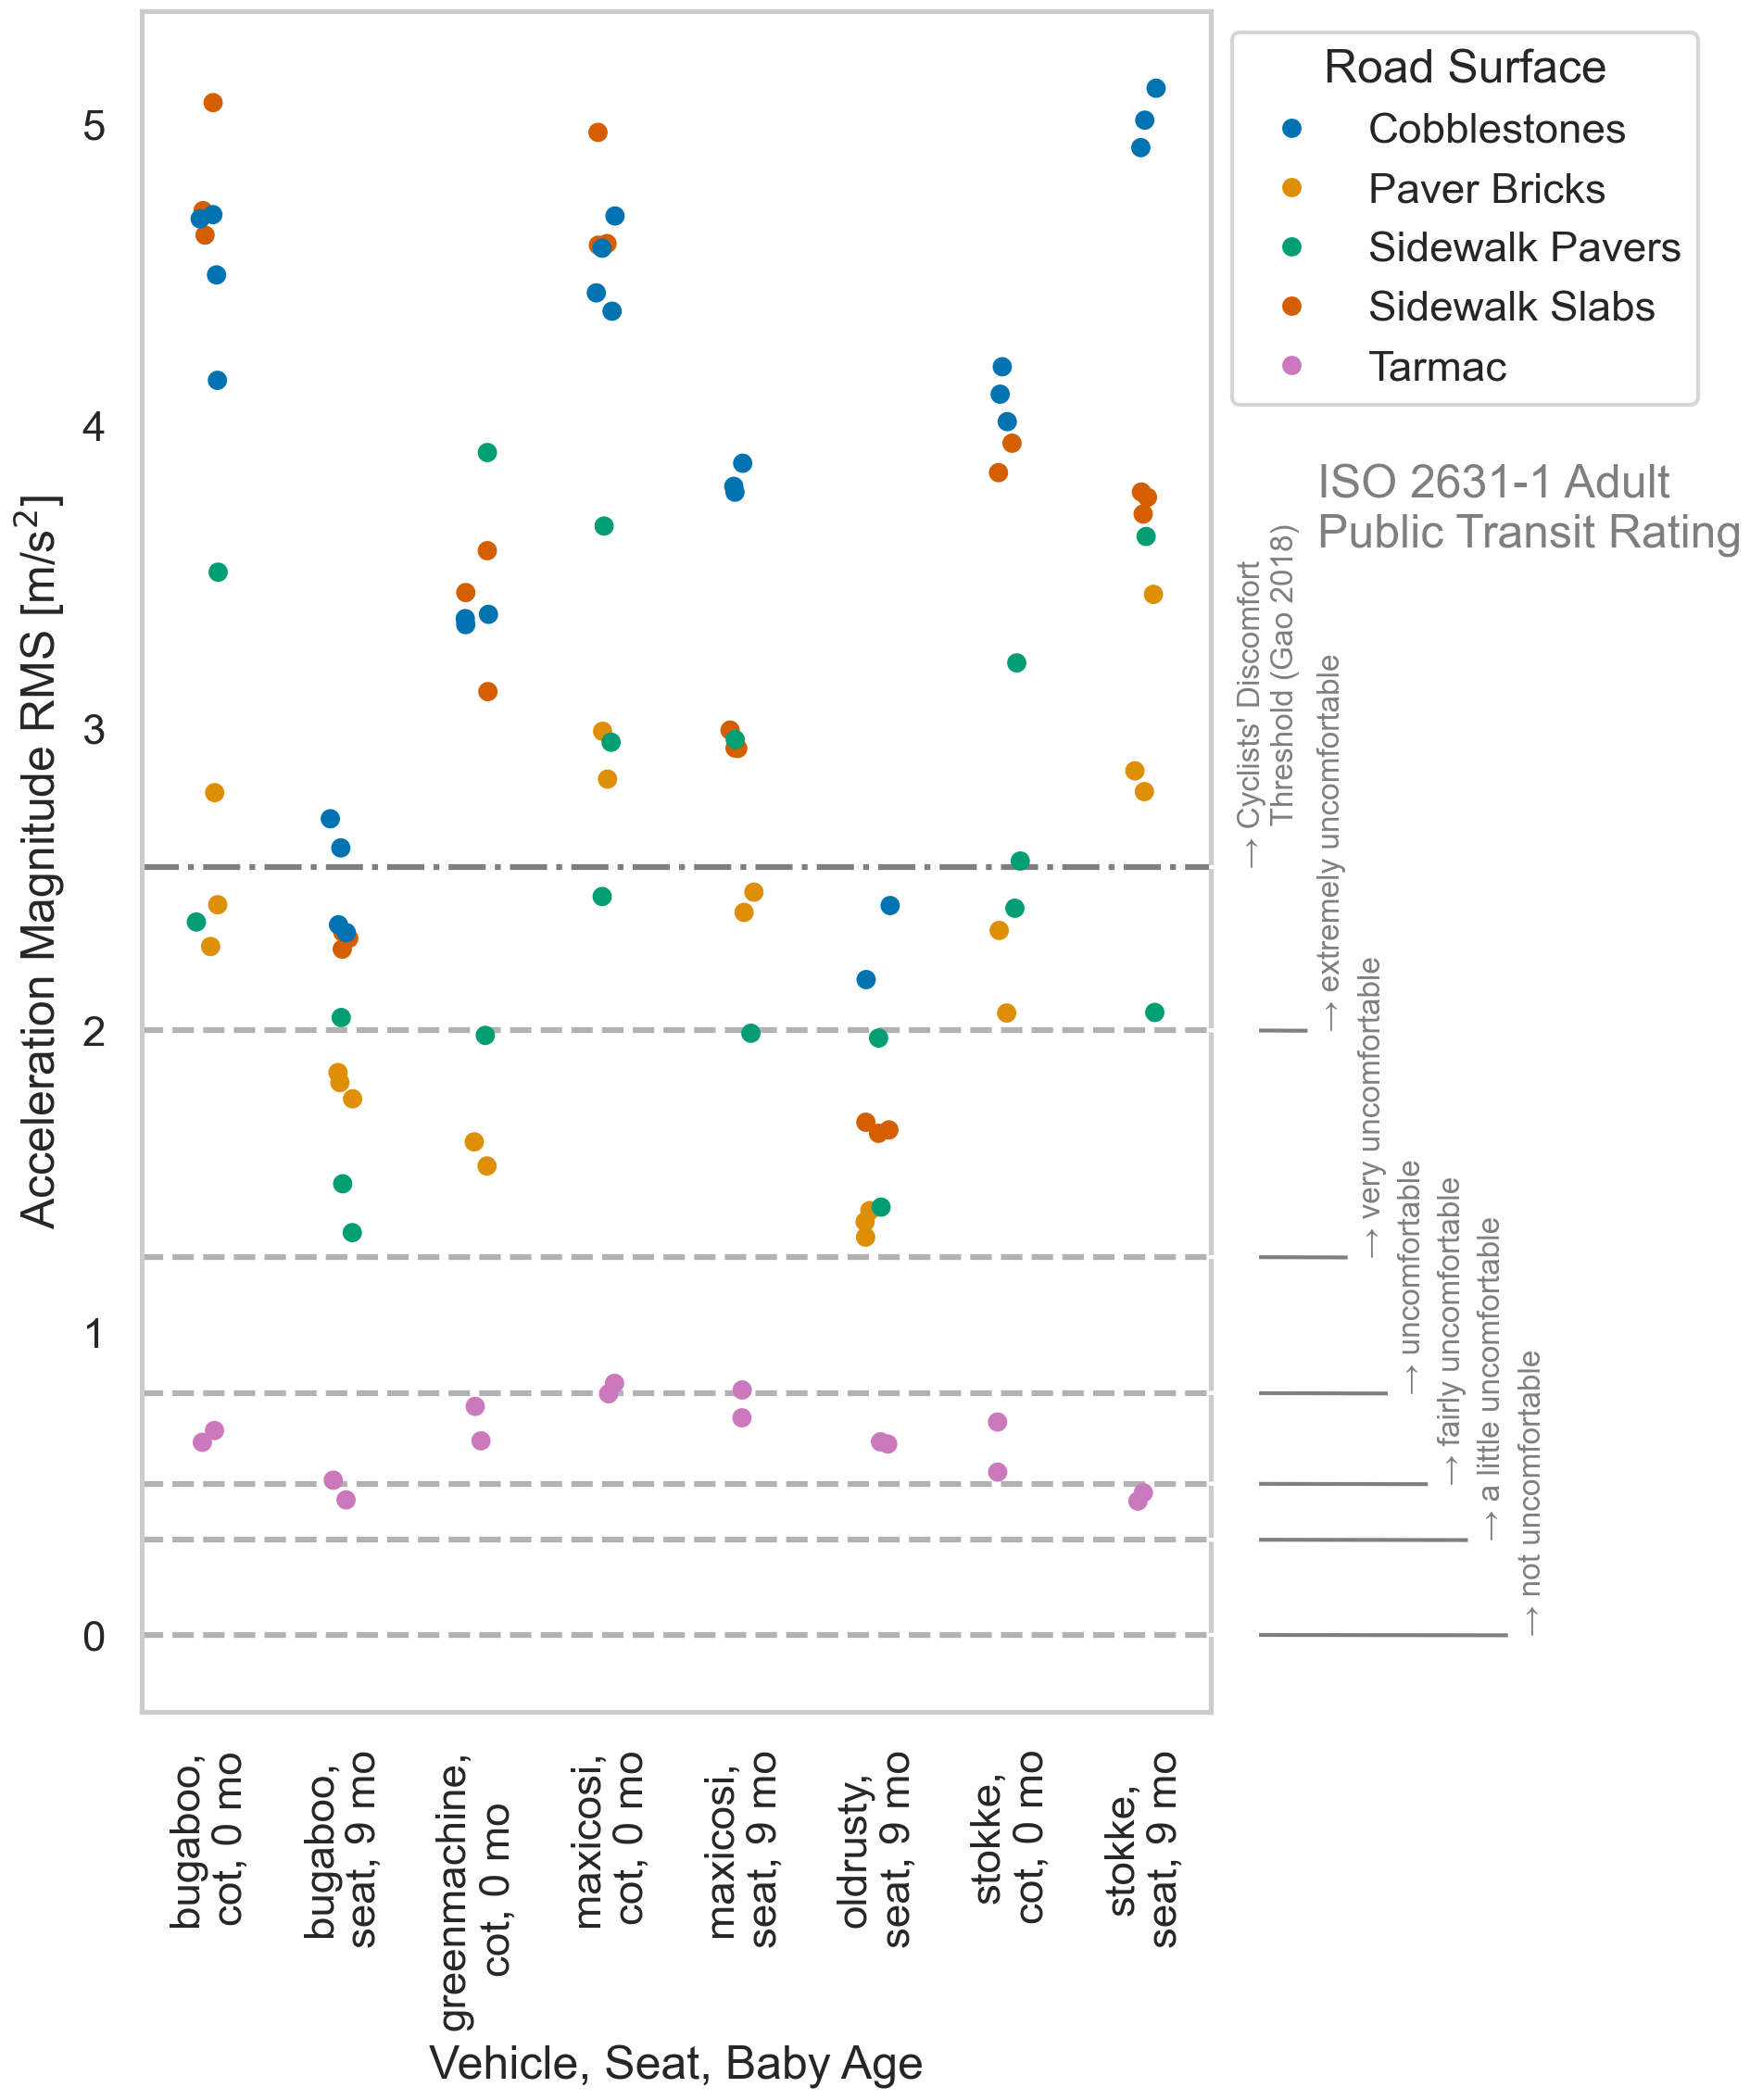
\includegraphics[width=160mm]{fig/SeatBotacc_ver-rms-comfort-stroller-compare-all.png}
  \caption{ISO~2631-1 weighted seat pan magnitude RMS acceleration of all
  stroller repetitions with colour representing the road surface. The horizontal
  dashed lines are the lower bound of the ISO~2631-1 ``comfort zones'' for
  adults seated erectly experiencing vibrations in public transit. The
  horizontal dashed dotted line is the cyclists' vibration discomfort threshold
  as reported by Gao et. al~\cite{Gao2018}.}
  \label{fig:comfort-stroller}
\end{figure}

Both cargo bicycles ridden at any tested speed over paver bricks, as well as the
Keiler with Pebble ridden over tarmac at high speed fall into the category
``extremely uncomfortable''. Those are also above the cyclist discomfort
threshold. The other vehicle setups fall between ``fairly uncomfortable'' and
``very uncomfortable'' over tarmac for all tested speeds. The Urban Arrow with
Melia performs, on average, the best on paver bricks and tarmac at all tested
speeds.
%
\begin{figure}
  \centering
  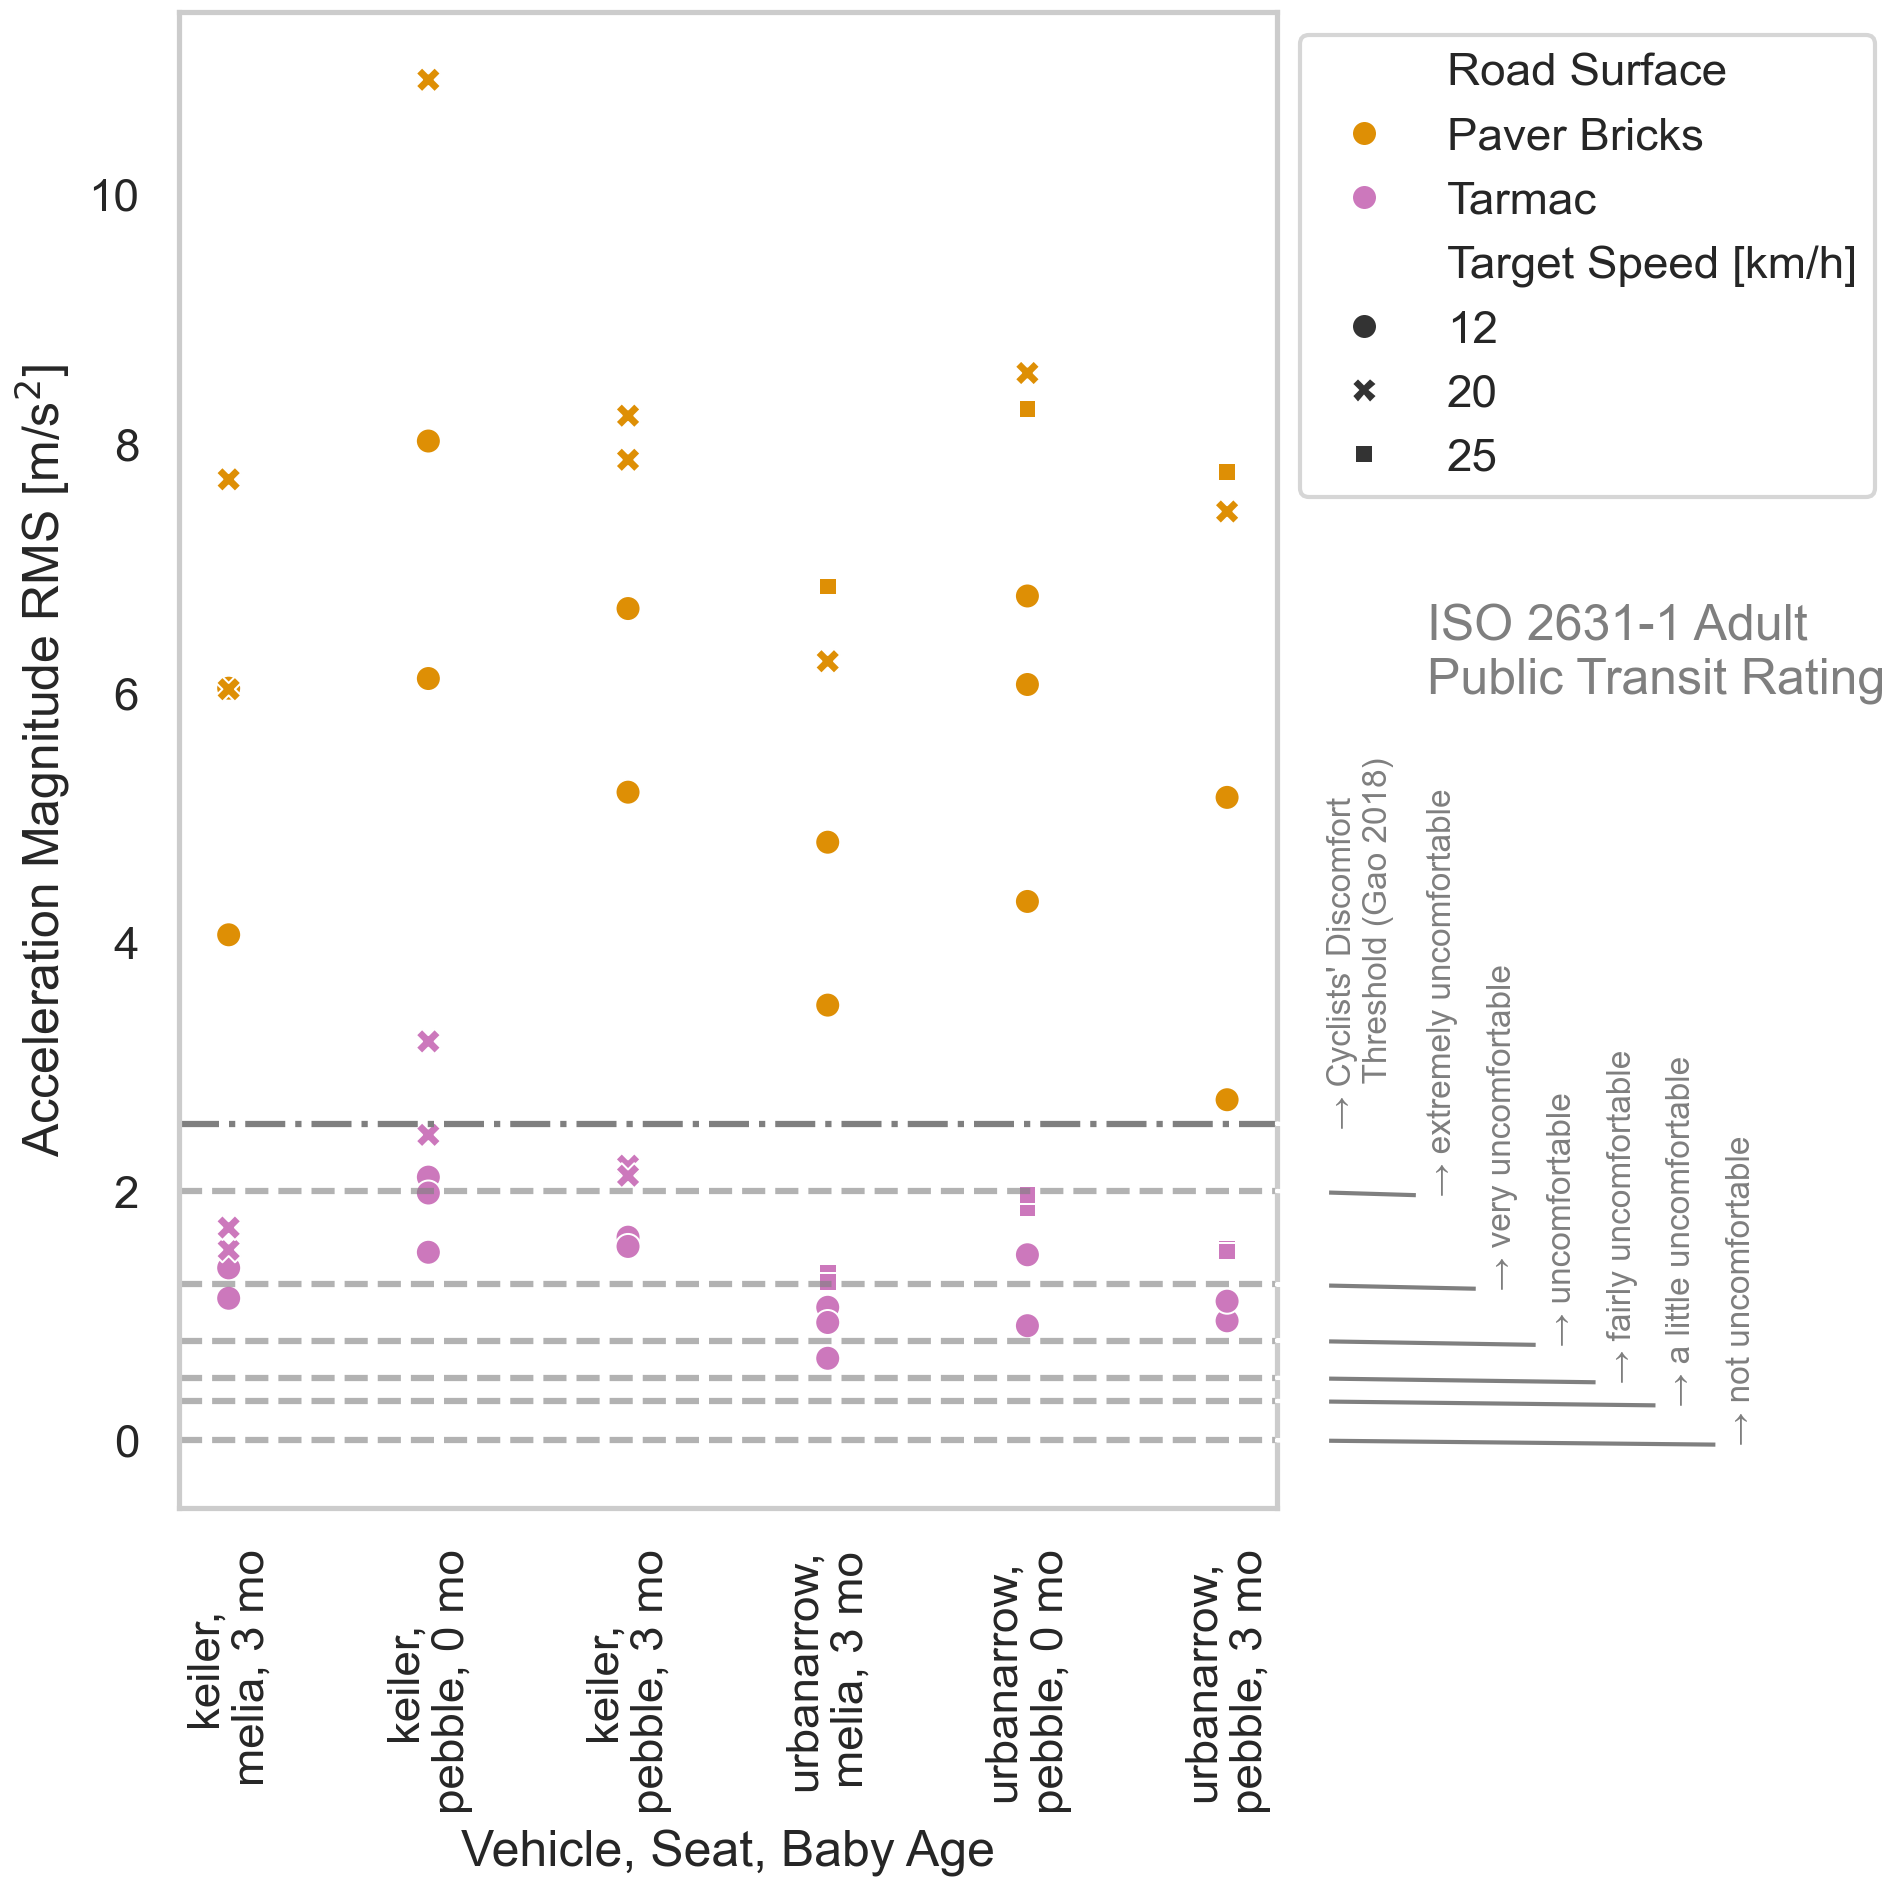
\includegraphics[width=160mm]{fig/SeatBotacc_ver-rms-comfort-bicycle-compare-all.png}
  \caption{ISO~2631-1 weighted seat pan magnitude RMS acceleration of all cargo
  bicycle repetitions with colour representing road surface and marker style
  representing the target speed. The horizontal dashed lines with the upper
  bound of the ISO~2631-1 ``comfort zones'' for adults seated erectly
  experiencing vibrations in public transit. The horizontal dashed-dotted line
  is the cyclists' vibration discomfort threshold as reported by
  Gao~et.~al~\cite{Gao2018}.}
  \label{fig:comfort-bicycle}
\end{figure}

\subsection{Statistical Results}
\label{sec:statistical-results}
%
For strollers, Table~\ref{tab:stroller-ols} shows the results of the 11 degrees
of freedom statistical model for the 104 repetitions~(\(R^2=0.867,F=54.69\)).
Both categorical variables have significant effects. The intercept gives the
mean acceleration of the Green Machine pushed over tarmac, which is not
significant. All road surfaces cause significantly higher acceleration than
tarmac, with cobblestones having the largest relative effect
(3.0~\si{\mps\squared} larger), followed by sidewalk slabs
(2.7~\si{\mps\squared} larger), sidewalk pavers (1.8~\si{\mps\squared} larger),
and paver bricks (1.6~\si{\mps\squared} larger). The `Bugaboo, Seat, 9 mo' and
`Maxi-Cosi, Seat, 9 mo' are not significantly different from the `Green Machine,
Cot, 0 mo' but the other strollers are. The `Old Rusty, Seat, 9 mo' and
`Bugaboo, Cot, 0 mo' showed significantly lower RMS acceleration than `Green
Machine, Cot, 0 mo' by 0.8 and 0.5~\si{\mps\squared}, respectively. The
remaining strollers have higher accelerations than the `Green Machine, Cot, 0
Mo' on tarmac: `Maxi-Cosi, Cot, 0 mo' (1.1~\si{\mps\squared}), `Bugaboo, Cot, 0
mo' (1.0~\si{\mps\squared}), `Stokke, Seat, 9 mo' (1.0~\si{\mps\squared}), and
`Stokke, Seat, 0 mo' (0.6~\si{\mps\squared}).
%
\begin{table}
  \centering
  \caption{Ordinary Linear Regression Results for Strollers. Tarmac and Green
  Machine (with Cot 0 month) are the references for the categorical Road Surface and
  Stroller variables, respectively. The columns give the effect \(\beta\), standard
  error, T-statistic, p-value, and the 95\% confidence interval.}
  \label{tab:stroller-ols}
\begin{tabular}{lcccccc}
\toprule
& \textbf{coef} & \textbf{std err} & \textbf{t} & \textbf{P$> |$t$|$} & \textbf{[0.025} & \textbf{0.975]}  \\
\midrule
\textbf{Intercept}                                                                                     &       0.2212  &        0.188     &     1.177  &         0.242        &       -0.152    &        0.595     \\
Cobblestones                                     &       3.0117  &        0.163     &    18.473  &         0.000        &        2.688    &        3.336     \\
Paver Bricks                                     &       1.6000  &        0.172     &     9.299  &         0.000        &        1.258    &        1.942     \\
Sidewalk Pavers                                  &       1.7566  &        0.174     &    10.092  &         0.000        &        1.411    &        2.102     \\
Sidewalk Slabs                                   &       2.7754  &        0.167     &    16.637  &         0.000        &        2.444    &        3.107     \\
Bugaboo, cot, 0 mo   &       0.9706  &        0.202     &     4.813  &         0.000        &        0.570    &        1.371     \\
Bugaboo, seat, 9 mo  &      -0.5065  &        0.199     &    -2.551  &         0.012        &       -0.901    &       -0.112     \\
Maxi-Cosi, cot, 0 mo  &       1.0795  &        0.202     &     5.353  &         0.000        &        0.679    &        1.480     \\
Maxi-Cosi, seat, 9 mo &       0.3012  &        0.209     &     1.441  &         0.153        &       -0.114    &        0.716     \\
Old Rusty, seat, 9 mo &      -0.7551  &        0.209     &    -3.605  &         0.001        &       -1.171    &       -0.339     \\
Stokke, cot, 0 mo     &       0.5766  &        0.209     &     2.753  &         0.007        &        0.161    &        0.993     \\
Stokke, seat, 9 mo     &       0.9706  &        0.205     &     4.731  &         0.000        &        0.563    &        1.378     \\
\bottomrule
\end{tabular}
\end{table}

For cargo bicycles, Table~\ref{tab:bicycle-ols} shows the results of the 8
degree of freedom statistical model for the 50
repetitions~(\(R^2=0.925,F=63.17\)). The categorical variable for vehicle setup
has significant effects, the categorical variable for road surface alone does
not, but the interaction of speed with road surface does have significant
effects. The intercept should be zero because there is no vertical vibration
when the speed is zero which aligns with the intercept not being significantly
different than zero. Speed is not a significant predictor on tarmac, but the
interaction variable shows that 0.8~\si{\mps\squared} is gained in acceleration
for each 1~\si{\kph} increase on paver bricks. The Urban Arrow with the 3~mo
infant in either seat has significant difference to the `Keiler, Pebble, 3~mo',
both showing reduction in relative acceleration. If the 0~mo dummy is used in
the Keiler with the Pebble there is significantly higher vibration.
%
\begin{table}
  \centering
  \caption{Ordinary Linear Regression Results for Cargo Bicycles. Tarmac and
  `Keiler, Pebble, 3 mo' are the references for the categorical Road Surface
  and Cargo Bicycle variables, respectively. The columns give the effect
  \(\kappa\), standard error, T-statistic, p-value, and the 95\% confidence
  interval.}
  \label{tab:bicycle-ols}
\begin{tabular}{lcccccc}
\toprule
& \textbf{coef} & \textbf{std err} & \textbf{t} & \textbf{P$> |$t$|$} & \textbf{[0.025} & \textbf{0.975]}  \\
\midrule
\textbf{Intercept}                                                                                          &       0.8067  &        0.643     &     1.255  &         0.216        &       -0.491    &        2.104     \\
Paver Bricks                                          &       1.2956  &        0.889     &     1.457  &         0.153        &       -0.500    &        3.091     \\
Keiler, Pebble, 0 mo     &       0.8664  &        0.415     &     2.085  &         0.043        &        0.027    &        1.705     \\
Keiler, Melia, 3 mo        &      -0.5060  &        0.415     &    -1.219  &         0.230        &       -1.344    &        0.332     \\
Urban Arrow, Pebble, 0 mo &      -0.0512  &        0.404     &    -0.127  &         0.900        &       -0.867    &        0.764     \\
Urban Arrow, Pebble, 3 mo &      -0.8895  &        0.415     &    -2.141  &         0.038        &       -1.728    &       -0.051     \\
Urban Arrow, Melia, 3 mo    &      -1.1357  &        0.403     &    -2.819  &         0.007        &       -1.949    &       -0.322     \\
Mean Speed [m/s]                                                                              &       0.2034  &        0.116     &     1.747  &         0.088        &       -0.032    &        0.439     \\
Mean Speed\(\times\)Road Surface                    &       0.7803  &        0.180     &     4.338  &         0.000        &        0.417    &        1.144     \\
\bottomrule
\end{tabular}
  \end{table}
  
Given that the vehicle setup (\(x_\textrm{Stroller}\) and \(x_\textrm{Cargo
Bicycle}\)) has a significant effect, we performed a post-hoc analysis to
compare vehicles on each road surface. Table~\ref{tab:sig-group-stroller},
derived from Figure~\ref{fig:tukey-stroller} in Appendix~\ref{app:compare},
shows the groupings of non-significant comparisons for a Tukey Range Test among
the strollers.
Old Rusty and `Bugaboo, Seat, 9 mo' and the Green Machine perform generally
better (significantly) than the other vehicles, shown by the ``overall''
ranking.
For cobblestones, this is also true as well as: 1) the `Stokke, Seat, 9 mo' is
the worst stroller tested and, interestingly, the heavier dummy performs worse
than the lighter one; 2) the 9-month dummy experiences lower acceleration in the
Bugaboo and Maxi-Cosi.
For paver bricks: 1) Old Rusty, `Bugaboo, Seat, 9 mo', and Green Machine are
again the best and 2) `Stokke, Seat, 9 mo' sees higher acceleration than the
0-month configuration.
For sidewalk pavers, there was no significant difference among all the
strollers. For sidewalk slabs: 1) Old Rusty is the best and Bugaboo the second
best; 2) the 0-month in the Bugaboo and Maxi-Cosi see more than the 9-month in
the same vehicle, respectively; and 3) no difference in Stokke when comparing
dummy sizes. For tarmac: 1) the Green Machine, `Bugaboo, Seat, 9 mo', and
`Stokke, Seat, 9 mo' are better than Maxi-Cosi with either dummy size; and 2)
the Green Machine is better than the `Bugaboo, Cot, 0 mo'.
%
\begin{table}
\centering
\caption{Stroller Significance Ranking Groups (based on
Figure~\ref{fig:tukey-stroller}). The numbers indicate the group where there is
no significant difference with 1 being the best (lower acceleration) and 8 being
the worst (higher acceleration). The ``Overall'' column gives an overall ranking
based on the mean ranking of the other columns.}
\label{tab:sig-group-stroller}
\begin{tabular}{lcccccc}
  \toprule
                          &         &              & Paver  & Sidewalk & Sidewalk & \\
  Vehicle Setup           & Overall & Cobblestones & Bricks & Pavers   & Slabs    & Tarmac \\
  \midrule
  Bugaboo, cot, 0 mo        & 7 & 5-7 & 4-8 & 1-8 & 7-8 & 2-8 \\
  Bugaboo, seat, 9 mo       & 2 & 1-2 & 1-5 & 1-8 & 2   & 1-6 \\
  Green Machine, cot, 0 mo  & 3 & 3   & 1-3 & 1-8 & 3-4 & 1-5 \\
  Maxi-Cosi, seat, 0 mo     & 8 & 5-7 & 5-8 & 1-8 & 7-8 & 4-8 \\
  Maxi-Cosi, seat, 9 mo     & 4 & 4-5 & 3-8 & 1-8 & 3-4 & 4-8 \\
  Old Rusty, seat, 9 mo     & 1 & 1-2 & 1-3 & 1-8 & 1   & 1-8 \\
  Stokke, cot, 0 mo         & 5 & 4-7 & 3-6 & 1-8 & 5-6 & 1-8 \\
  Stokke, seat, 9 mo        & 6 & 8   & 6-8 & 1-8 & 5-6 & 1-6 \\
  \bottomrule
\end{tabular}
\end{table}

When comparing cargo bicycles (Table~\ref{tab:sig-group-bicycle}), most
vehicle setups deliver similar acceleration to the seat pan when ridden over the
same surface at the same target speed. For low speed on tarmac, the Urban Arrow
with Melia and a 3-month dummy has significantly less acceleration
than the Keiler with Pebble and 0-month dummy. There is no significant
difference in any vehicle setups at low speed on paver bricks. At higher speeds,
the Urban Arrow and Keiler with Melia and the 3-month dummy are
significantly better than the Keiler with Pebble and the 0-month dummy on paver
bricks and on tarmac. It is important to point out that there is no significant
difference when simply swapping the seat for the 3-month dummy, which does not
support the hypothesis in Section~\ref{sec:health-assesment}.
%
\begin{table}
\centering
\caption{Cargo Bicycle Significance Ranking Groups (based on
Figure~\ref{fig:tukey-bicycle}). The numbers indicate the group where there is
no significant difference with 1 being the best (lower acceleration) and 6 being
the worst (higher acceleration). The ``Overall'' column gives an overall ranking
based on the mean ranking of the other columns. Note that the mean ranking is
very close for all cargo bicycles.}
\label{tab:sig-group-bicycle}
\begin{tabular}{lccccc}
     \toprule
                                &         & Paver Bricks & Tarmac    & Paver Bricks & Tarmac \\
     Vehicle Setup              & Overall & Low Speed    & Low Speed & High Speed   & High Speed \\
     \midrule
     Keiler, Melia, 3 mo       & 2 & 1-6 & 1-6 & 1-5 & 1-5\\
     Keiler, Pebble, 0 mo      & 6 & 1-6 & 2-6 & 3-6 & 5-6\\
     Keiler, Pebble, 3 mo      & 5 & 1-6 & 1-6 & 1-6 & 1-6\\
     Urban Arrow, Melia, 3 mo  & 1 & 1-6 & 1-5 & 1-5 & 1-5\\
     Urban Arrow, Pebble, 0 mo & 4 & 1-6 & 1-6 & 1-6 & 1-5\\
     Urban Arrow, Pebble, 3 mo & 2 & 1-6 & 1-6 & 1-5 & 1-5\\
     \bottomrule
\end{tabular}
\end{table}

\section{Discussion}
%
We have presented a comprehensive set of acceleration measurements from
experiments that simulate vibrations experienced by infants in the 0-9-month age and mass range during transportation in strollers and cargo bicycles. We compared
the average magnitude of vertical and total acceleration at the seat pan across
a variety of road surfaces and seats at typical travel speeds. ISO~2631-1
weighted average acceleration ranged from \SIrange{0.4}{10.7}{\mps\squared}
across all tested scenarios. Strollers induced \SIrange{0.4}{5.0}{\mps\squared}
for a mean walking speed of 5.3~\si{\kph}. Cargo bicycles induced
\SIrange{0.6}{10.7}{\mps\squared} over a speed range of \SIrange{12}{25}{\kph}.

\subsection{Surface and Speed}
%
Travelling over a tarmac surface showed the least vibration in all types of
vehicles at any speed with a range of \SIrange{0.4}{1.2}{\mps\squared}. For
strollers, the roughest surfaces being cobblestones and sidewalk slabs with
large gaps caused 5\(\times\) the acceleration experienced on tarmac, reaching
5.0~\si{\mps\squared}. More common surfaces, sidewalk pavers and
paver bricks, reach values up to 3~\si{\mps\squared}.

For cargo bicycles, travelling over paver bricks at the same speeds can
quadruple average acceleration relative to tarmac. Travelling at the maximum
allowed speed of an electric cargo bicycle (25 \si{\kph}) over paver bricks
caused average accelerations that exceeded 8~\si{\mps\squared}. Additionally, the
effect of speed on vibration was significant for paver bricks but not for tarmac.

Whereas speed strongly affected the acceleration amplitude, it had lesser effect
on the peak frequency and the bandwidth. Peak frequency at the highest speed was
1.25\(\times\) higher for tarmac than paver bricks and bandwidth approximately
doubled for paver bricks relative to tarmac at high speeds. This suggests that
oscillations induced by the systems tested may have strong influence relative to
dominant frequencies resulting from the road surface.

\subsection{Baby Mass}
%
The size of the dummy (mass and build) had no obvious systematic effect on the
average acceleration at the seat pan. These vibrations are transmitted to
infant's body, and the physical properties (mass, stiffness, and damping) of the
infant's body determine whether this excitation is amplified or not and which
body segment is more affected. Tests with more realistic dummies or real infants
along with comparisons of equivalent vehicle setups are necessary to investigate
how the infant itself moves when excited by this level of vibration. This
information is not readily available in the literature and may be difficult to
acquire due to ethical limitations and the absence of validated infant dummies.
The only effect that stood out for mass was that, counter-intuitively, the
lighter dummy had less acceleration than the heavier dummy for the Stokke
stroller, but this may well be explained by the different stroller
configurations tested for the two body sizes.

\subsection{Health}
%
Vertical RMS acceleration on uneven surfaces can be relatively large compared to
the smoothest experience on tarmac. When we compare the vibration measured for
infants in strollers and cargo bicycles with the ISO~2631-1 standard vibration
``health risk zone'' as defined for long-term exposure of adults seated erectly,
we see that:
%
\begin{itemize}
    \item only strollers pushed over tarmac at 5~\si{\kph} had average
    acceleration below the ``health risk zone" for 4~\si{\hour} daily duration,
    \item walking with an infant in a stroller on cobblestones and sidewalk
    slabs can exceed the ``health risk zone'' within 20~\si{\min} to
    1~\si{\hour}, depending on the stroller model and the age of the child,
    \item cargo bicycles ridden at \SIrange{12}{25}{\kph} over tarmac delivered
    accelerations below the 1~\si{\hour} ``health risk zone'' for all but the
    Keiler with the newborn,
    \item cycling with an infant in a cargo bicycle on tarmac at 12~\si{\kph}
    can be maintained for approximately two hours before exceeding the ``health
    risk zone'',
    \item cargo bicycles ridden at \SI{12}{\kph} over paver bricks delivered
    accelerations exceed the 10~\si{\min} ``health risk zone'' for three of the
    6 vehicle setups and range between \SI{1}{\hour} to \SI{20}{\minute}
    otherwise, and
    \item cycling with an infant in a cargo bicycle on paver bricks at
    \SIrange{20}{25}{\kph} for 10~\si{\min} gives the infant a vibration load
    that equals or exceeds the ``health risk zone''. 
\end{itemize}

When utilizing the ISO~2631-1 guidance, we can conclude that strollers can be
pushed over paver bricks and sidewalk pavers continuously for no more than half
an hour. On extreme surfaces like cobblestones and sidewalk slabs, strollers
should be pushed slower than 5~\si{\kph} with a duration of maximal
10~\si{\min}. A stroller can be walked continuously for four hours only on
tarmac, and only if the infant is lying in the cot. If the infant is sitting,
the parent/caregiver would need to consider appropriate breaks to allow the
infant to move. Cargo bicycles carrying infants over paver bricks should slow
down to 12~\si{\kph} or preferably less, and the duration should be kept under
10~\si{\min}. When riding a cargo bicycle over tarmac at 20~\si{\kph}, the
duration should be kept under 1~\si{\hour}. At 12~\si{\kph}, cargo bicycles can
ride over tarmac for maximal 2~\si{\hour}.

The largest unweighted RMS vertical acceleration we recorded at the seat pan was
\SI{12.6}{\mps\squared}. Tsuijuchi et~al.~\cite{Tsujiuchi2014} studied inflicted
head injury by shaking trauma and give evidence based on finite element
modelling that shaking an infant at the chest with an unsupported head at
\SI{14}{\mps\squared} for \SI{2}{\second} could rupture brain bridging veins.
This is a largely different scenario with an unsupported head and accelerations
acting in different directions than in our experiments, yet it is worrisome that
the acceleration magnitudes are of the same order of magnitude.

\subsection{Comfort}
%
When considering comfort, the ISO~2631-1 guidelines estimate that adults would
report the vibrations experienced in strollers and bicycles as uncomfortable.
For strollers, the vibrations over tarmac would be rated ``fairly
uncomfortable'' and all other road surfaces would be ``very'' or ``extremely
uncomfortable''. When riding a cargo bicycle over paver bricks, the vibrations
would be rated as ``extremely uncomfortable'' and over tarmac spans ``fairly``
to ``extremely''. The ISO~2631-1 comfort rating scale is derived from adult
subjective ratings of vibrations felt when riding public transit for an
unspecified duration, so we question whether the scale is appropriate for
typical strolling and cycling durations. Furthermore, the standard extensively
emphasises that comfort perception depends on many interacting factors.
Gao~et~al.~\cite{Gao2018} report that cyclists do not rate vibrations as
extremely uncomfortable on normal road surfaces, indicating a possible
contradiction, especially given a bicycle saddle is generally perceived less
comfortable than a chair-style seat used in the standard development. Lastly, it
is not readily possible to assess subjective comfort directly from infants so we
can only extrapolate from children and adult experience.

\subsection{Vehicle and Seat Design}
%
Different combinations of vehicle, seat, and baby mass cause different average
vertical accelerations at the seat pan. We are only able to compare vehicle
setups, other than comparing the same two different baby seats in both cargo
bicycles. A striking discovery is that the two tested 1970s strollers
significantly outperformed many of the modern stroller setups on most road
surfaces. The vintage strollers had more sophisticated suspension systems that
used springs, straps, and larger wheels. Stroller manufacturers may have reduced
suspension as a side effect of decreasing the size and weight of strollers and
introducing swivelling front wheels (which makes steering lighter but which made
manufacturers drop suspension solutions like these in the vintages products). As
an example, the ``Old Rusty'' stroller was the only one that did not exceed the
1~\si{\hour} health risk line for any road surface.

Both the Bugaboo and Maxi-Cosi strollers showed lower accelerations for the
heavier baby, as expected, but the Stokke stroller showed the opposite trend for
cobblestones and paver bricks. This points to design choices in the seated
configuration that may excite resonance on certain surface profiles. The
`Bugaboo, Seat, 9 mo' configuration performed better than the other modern
strollers for all non-tarmac road surfaces. The Urban Arrow performed better
than Keiler on tarmac but there was no difference on paver bricks. Additionally,
there was no difference between different seats for the 3-month-old infant. The
performance of a vehicle setup was not necessarily constant with respect to cot
or seat configuration; contrarily, performance was often significantly different
when converting for different baby ages. This may be due to designs being
optimised for one configuration.

\subsection{ISO Frequency Weighting and Bandwidth}
%
We report RMS accelerations as well as the ISO~2631-1 weighted accelerations for
comparison. Vibrations at frequencies between \SIrange{4}{11}{\hertz} showed to
have the largest unweighted magnitude, but there are substantial accelerations
at higher frequencies, as shown by the unweighted 80\% bandwidth. Our results
show substantial differences between RMS and VDV, highlighting the importance of
reviewing their meaning. These differences emerge from the high bandwidth of the
accelerations now measured, which greatly exceed the bandwidth of accelerations
measured with adults seated in cars (see e.g. Figure 2 in
\cite{griffin2004experimental}). Adult experiments investigating discomfort as a function of frequency, show that significant
discomfort can be measured across all tested frequencies, being up to 80 Hz
\cite{morioka2010frequency} or even up to 315~\si{\hertz}~\cite{morioka2006magnitude}
albeit with reduced sensitivity.

The ISO frequency weightings are defined for adults in more or less erect
postures with the head being unsupported, whereas we now studied dummies
representing infants from 0-9 months lying with the head directly supported. The
ISO~2631-1 weightings represent a reduced sensitivity above 8~\si{\hertz}, which
is associated with the vertical dynamics of erect seated subjects, and filter
out such high frequencies~\cite{toward2011transmission,mirakhorlo2022effects}.
However, adult experiments show greater discomfort for frequencies above
8~\si{\hertz} when lying with head supported with \SIrange{30}{90}{\degree} back
inclination compared to sitting erect without head support
\cite{BASRI2013inclined}. Higher frequencies have also been associated with
effects on the central nervous system. For instance, experiments on rats showed
brain injury visible in behaviour through functional impairment and in visual
changes of brain structures in postmortem dissection after exposure to prolonged
whole-body vibration at 30~\si{\hertz} and
5~\si{\mps\squared}~\cite{Yan2015_cumulative_brain_injury/j.jstrokecerebrovasdis.2015.08.007}.
In some conditions, the RMS exceeds the ISO Weighted RMS substantially,
warranting further research on the effects of higher frequencies, in particular
for conditions where the head is supported and for children. Meanwhile, a
conservative approach is to (also) consider the unweighted RMS in the design and
evaluation of transport means for very young children.

\section{Conclusion}
%
\subsection{Summary}
%
The results herein raise concerns about transporting infants in strollers and
cargo bicycles. If the user's behaviour is not adjusted to avoid rough surfaces
or to travel slowly over them when transporting an infant, there are potential
health risks and discomfort from daily and repeated exposure to large vibrations
over a longer time. However, there is no direct evidence that connects
whole-body vibration as measured in this study to infant harm or negative health
effects and discomfort, thus we can only extrapolate from the limited guidelines
on adults in occupational settings. We did measure vibrations that would not be
permitted for adults to maintain long-term occupational health, and it is
reasonable to believe we should not subject our infants to the same. Further
research to establish direct evidence to infant health and comfort would
possibly permit less conservative caution than we conclude below. 

It is well known that whole-body vibration can be attenuated with good
suspension design. We see this in the drastic historical evolution of
suspensions in automobiles, buses, trucks, and trains. We do not see this same
kind of attention to suspension in strollers, cargo bicycles, and baby seats for
these vehicles. Both walking and cycling are well known to offer great societal
and personal benefits over travelling by car, so it behoves us all to optimise
transport for infants in these two modes of transportation. 

\subsection{Recommendations}
%
Our conclusions result primarily from the recommended application of ISO~2631-1.
It is of utmost importance to recognise that this standard cautions against
extending the use of the standard to situations for which its supporting data
were not derived. The standard is based primarily on pre-1997 studies of adult
whole-body vibration in occupational durations (\SIrange{4}{8}{\hour} daily
dose) or during public transport.
%
\begin{quote}
  \textbf{The recommendations in standard ISO~2631-1 have not been based on or
  validated for infants, children, or young adults, nor for recumbent or
  reclined seating postures with the head supported. Additionally, the
  admissible durations for health are not validated for daily short durations or
  shorter lifetime accumulation that dominate stroller and cargo bicycle travel
  with infants. So, our recommendations must be taken with caution, at least
  until more research is done to improve the standard guidance.}
\end{quote}
%
Nevertheless, the following list provides recommendations for users,
researchers, designers, and manufacturers based on the findings of this paper
that we believe stand in spite of the standard's limitations:
%
\begin{enumerate}
    \item Manufacturers of strollers, cargo bicycles, and seats should test for
    vibrations for all expected surface types and ranges of relevant body sizes
    and postures to ensure that their designs isolate vibrations well for all use
    conditions. Testing across relevant body sizes is especially important for
    strollers, due to the high mass of the infant relative to the mass of the
    stroller.
    \item Manufacturers should collaborate in testing and report their results
    publicly, similar to the safety ratings of the automobile industry. For the
    combined use of cargo bicycles and baby seats, manufacturers should
    collaborate in this effort.
    \item Manufacturers and scientists should collaborate to develop metrics and
    testing procedures for the long-term goal of a new standard.
    \item Designers should ensure that adequate vibration isolation occurs for
    vehicles that have multiple configurations (e.g. recumbent vs. erect
    seating).
    \item Designers and manufacturers should incorporate better suspension
    systems, as currently occurring vibrations can be drastically reduced.
    Useful information may be derived from past designs with better suspension.
    \item New cycling roads and sidewalks should have a tarmac-like smoothness.
    Cobblestones should be avoided.
    \item Users should consider limiting their speed when walking with strollers
    or riding over surfaces rougher than tarmac, as bumpier surfaces aggravate
    accelerations.
    \item Users are suggested to limit the duration of transport over surfaces
    rougher than tarmac to periods that do not exceed 10-30 continuous minutes
    depending on the system (quality of suspension, larger tyres or wheels) and
    other countermeasures like adequate non-vibration breaks in between. When
    transporting over tarmac, continuous durations should not exceed 4 hours,
    and need to include regular breaks, if only to allow the infant to move free
    from the seat harness.
    \item Users should preferably ride any cargo bicycle at a speed of maximal
    12~\si{\kph} over surfaces rougher than tarmac. E-cargo bicycles can easily
    reach the maximum speed of 25~\si{\kph}. Infants should only be transported
    for short durations when riding over non-tarmac surfaces at these speeds.
    \item Standard ISO~2631-1 is not validated to characterise health and
    comfort effects of vibration for infants or children, for short travel
    durations, for vibration accumulation over only a small number of years, or
    for non-erect seating. However, this is the only available standard in the
    literature assessing health and comfort levels on vibrations, and should be
    used as a benchmark. More research should be done to enable the design of a
    standard on vibration that is applicable for infant transportation.
\end{enumerate}

\subsection{Acknowledgement}
%
Neil Mansfield, Jim Papadopoulos, Malte Rothhämel, Stefan Schwanitz, Idsart
Kingma, Darek Wieckowksi, Aernout Dijkstra-Hellinga, and  Clement Moe all
provided important feedback on the preprint that helped improve the paper. This
work was financially supported by VeiligheidNL under the ``Project Trillingen
bakfiets en wandelwagen.''

\subsection{Declaration of Interest Statement}
%
The authors report there are no competing interests to declare.

\subsection{Data Availability Statement}
%
The data will be made publicly available alongside publication.

\bibliographystyle{plain}
\bibliography{reference}

\newpage
\appendix

% Ensure subsections retain "A.1", "A.2", etc.
%\addcontentsline{toc}{section}{Appendix} % Optional: Add to TOC
%\renewcommand{\thesection}{A}
%\renewcommand{\thesubsection}{\thesection.\arabic{subsection}}

\section{Additional Exploratory Statistics}
\subsection{Effect of Speed}
%
Figure~\ref{fig:compare-bicycle-speed} shows the variation in ISO~2631-1
weighted vertical RMS acceleration across the tested speeds. On paver
bricks, the RMS acceleration increased by approximately 1.6\(\times\) when increasing
the speed from \SIrange{12}{25}{\kilo\meter\per\hour}.The effect of speed while cycling on tarmac was less drastic, but still showed a slight increase.
%
\begin{figure}
  \centering
  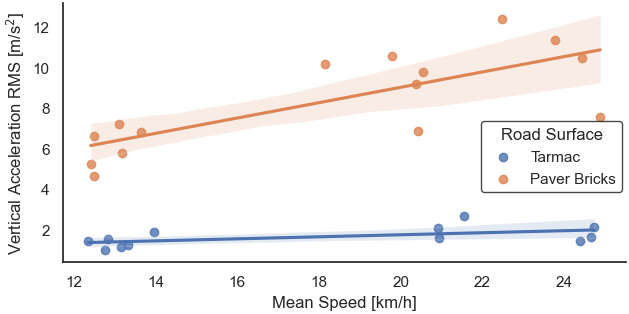
\includegraphics[width=160mm]{fig/SeatBotacc_ver-bicycle-speed-compare.png}
  \caption{Seat pan ISO 2631-1 weighted vertical acceleration RMS versus speed
  for all cargo bicycle repetitions. Shaded regions represent the 95\%
  confidence intervals from a simple linear regression that ignores
  \(x_\textrm{Cargo Bicycle}\).}
  \label{fig:compare-bicycle-speed}
\end{figure}

\subsection{Effect of Dummy Size}
%
Figure~\ref{fig:compare-baby-mass} shows the ISO~2631-1 weighted vertical RMS
acceleration for each repetition for all vehicles, and compares the dummy sizes.
Substantial variation has been shown to relate significantly to the surface and
within cargo bicycles, as well as to speed (see tables
\ref{tab:sig-group-stroller},\ref{tab:sig-group-bicycle}).
%There were larger accelerations in the bicycle (high speeds) versus the stroller (low speeds), likely mostly attributed to the different testing speeds. 
When comparing the vertical RMS acceleration values between cargo bicycles and
strollers, there are no obvious differences due to baby size, i.e. each dummy
size experienced a similar range of acceleration magnitudes when the vehicle type
and the road surface are ignored. For bicycles, the lightest dummy sometimes
experienced a higher acceleration than the heavier dummy, but high and low
accelerations were observed across the tested speed range.
%
\begin{figure}
  \centering
  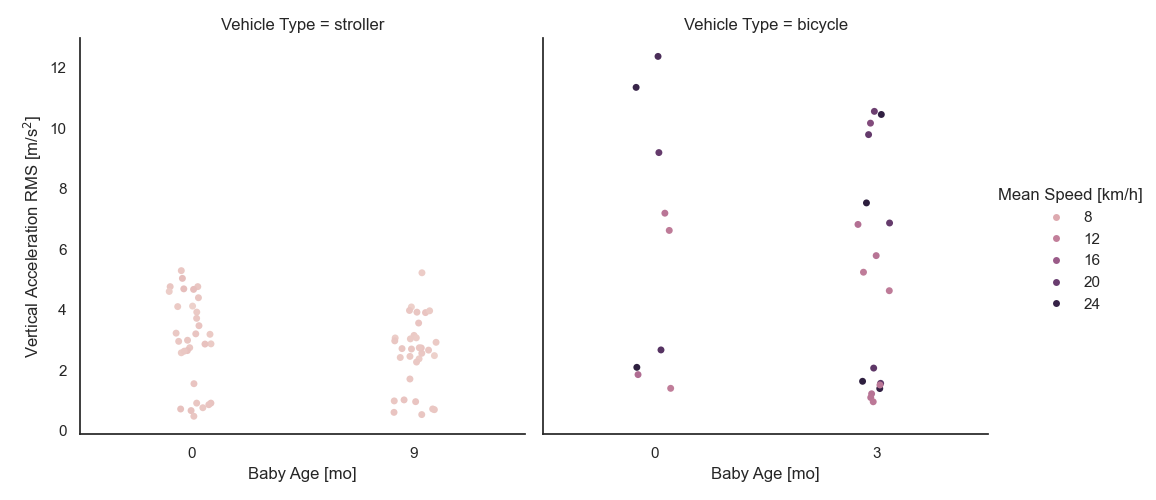
\includegraphics[width=160mm]{fig/SeatBotacc_ver-baby-mass-compare.png}
  \caption{Seat pan ISO~2631-1 weighted vertical RMS acceleration grouped by
  baby age (and thus size \& mass) for all repetitions with colour indicating
  the mean speed of the trial. The lightest colour dots are strollers (4 km/h) and the
  remaining are cargo bicycles (8-24 km/h).}
  \label{fig:compare-baby-mass}
\end{figure}

\subsection{Effect of Road Surface}
%
Figure~\ref{fig:compare-road-surface} shows ISO~2631-1 weighted vertical RMS
acceleration from repetitions grouped into the various road surfaces tested. All
vehicles were tested on paver bricks and tarmac, but only strollers were tested
on cobblestones, sidewalk pavers, and sidewalk slabs, i.e. light colour dots
(strollers are present in each column).
It is notable that tarmac almost always induced lower RMS acceleration than
other road types regardless of speed and vehicle type.
The sidewalk slabs and cobblestones have very similar acceleration ranges for
all strollers.
Paver bricks and sidewalk pavers appear to have a similar range of RMS
acceleration for the same 5~\si{\kilo\meter\per\hour} walking speeds.
Paver bricks cause relatively large accelerations at high travel speeds in
cargo bicycles. Paver bricks result in approximately 4-5\(\times\) higher accelerations compared to tarmac.
%
\begin{figure}
  \centering
  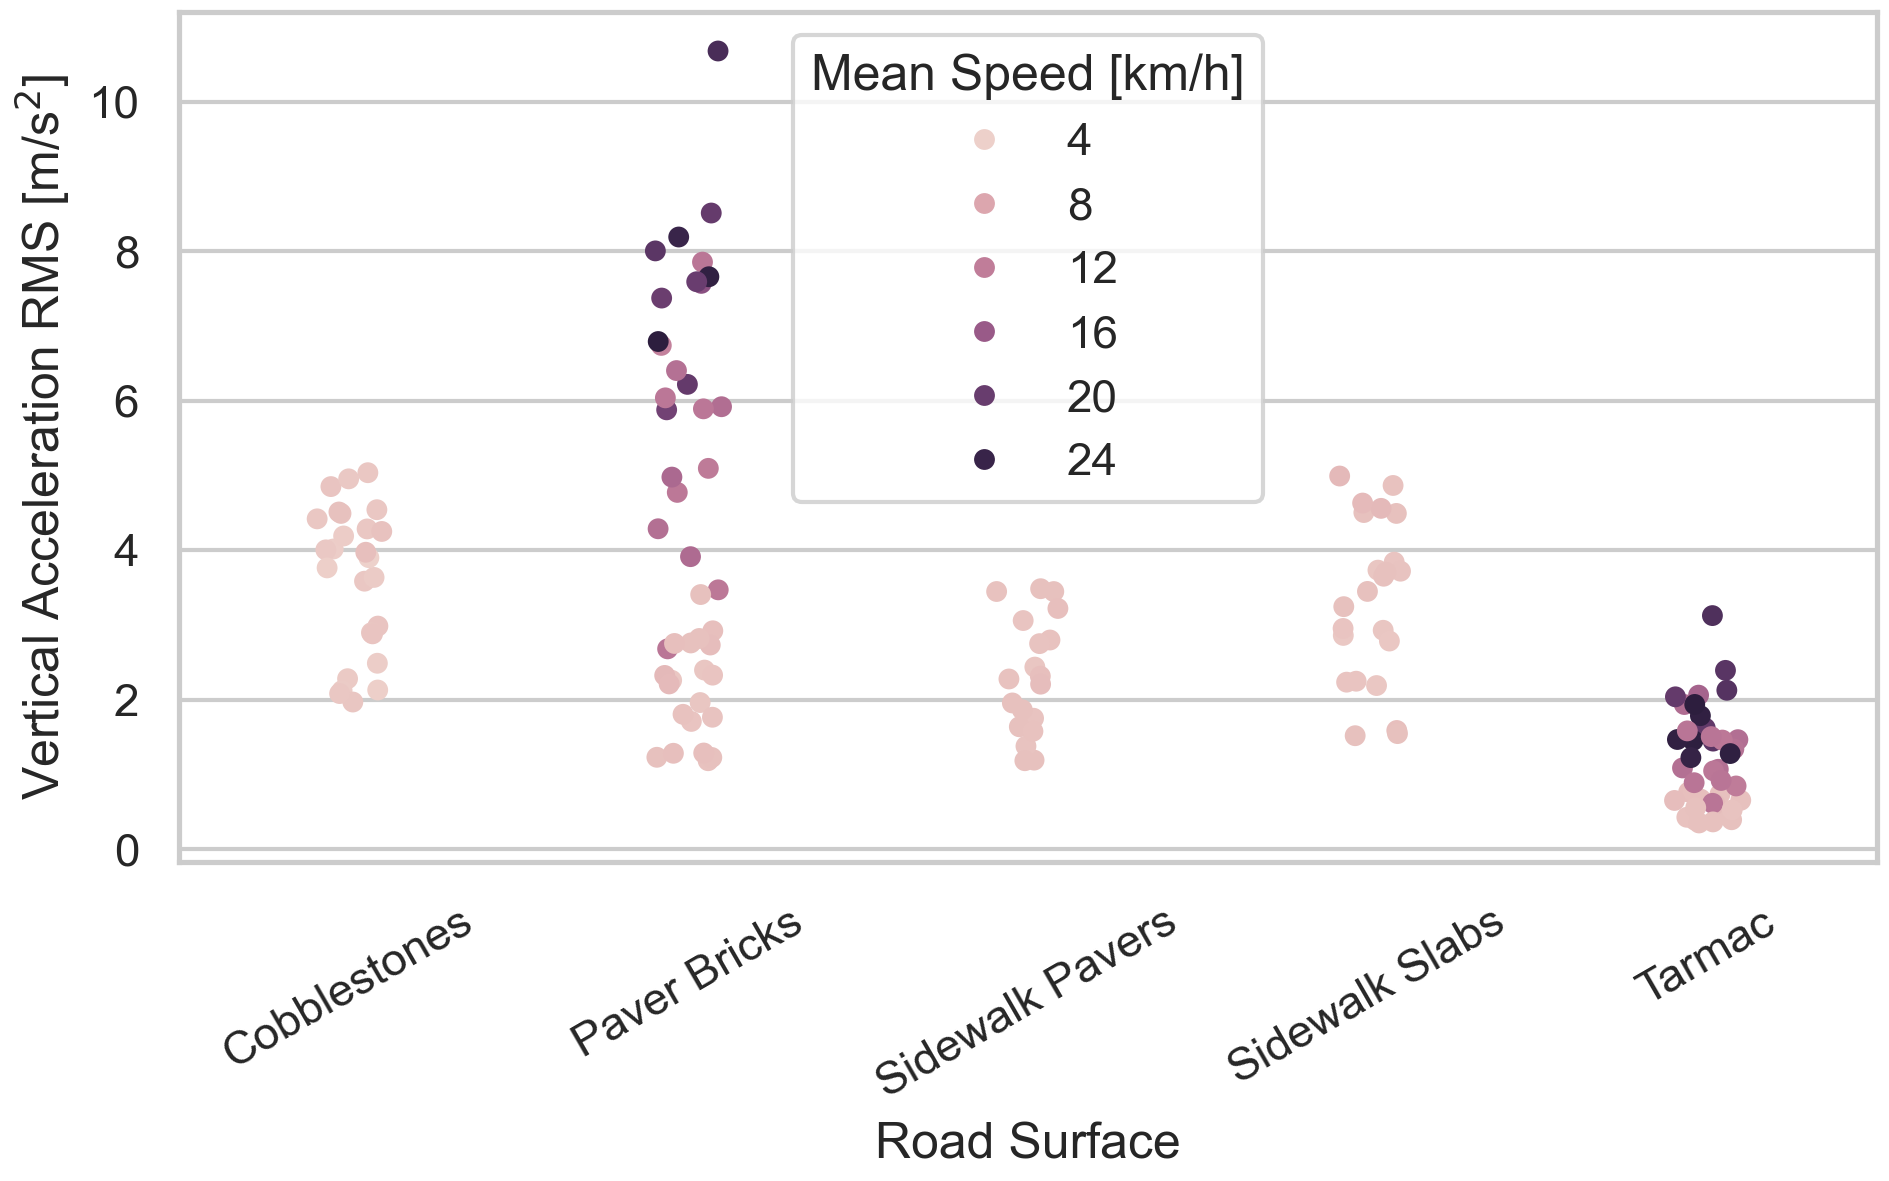
\includegraphics[width=160mm]{fig/SeatBotacc_ver-road-surface-compare.png}
  \caption{Seat pan ISO 2631-1 weighted vertical RMS acceleration grouped by
  road surface with colour indicating the mean speed of the repetition. The
  lightest colour dots are strollers (4 km/h), and the rest are cargo bicycles (8-24 km/h).}
  \label{fig:compare-road-surface}
\end{figure}

\newpage
\section{Vehicle Statistical Comparisons}
\label{app:compare}
%
Tukey Range Test multiple comparison plots. Horizontal lines indicate 95\%
confidence intervals. Non-overlapping confidence intervals indicate a
significant difference.
%
\begin{figure}[!ht]
  \centering
  \subcaptionbox{}{
  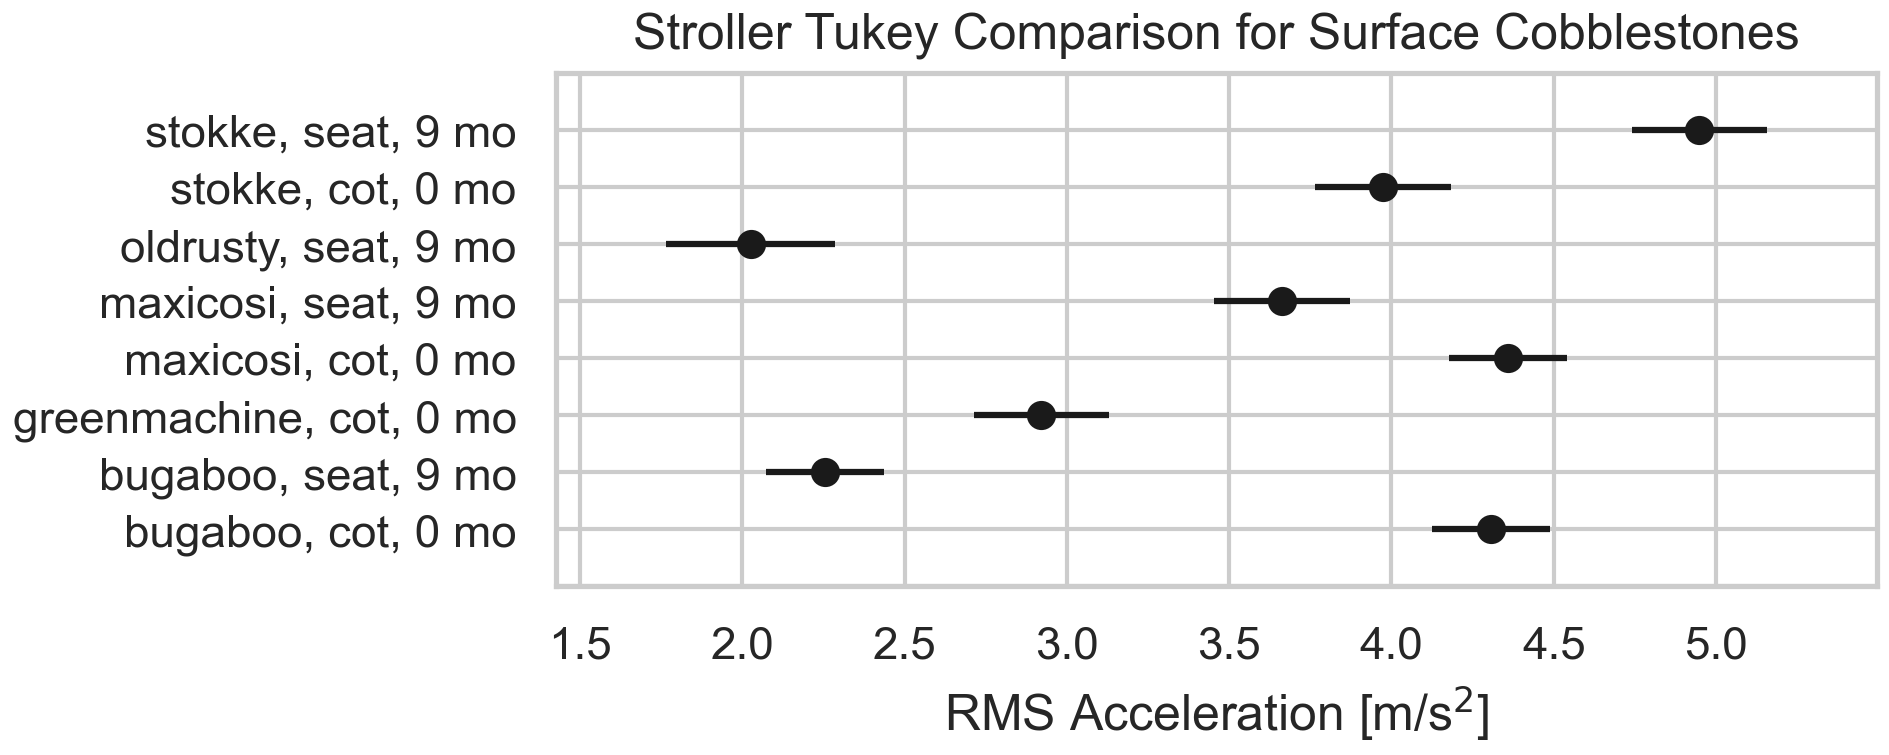
\includegraphics[width=90mm]{fig/tukey-SeatBotacc_ver-stroller-Cobblestones.png}}
  \subcaptionbox{}{
  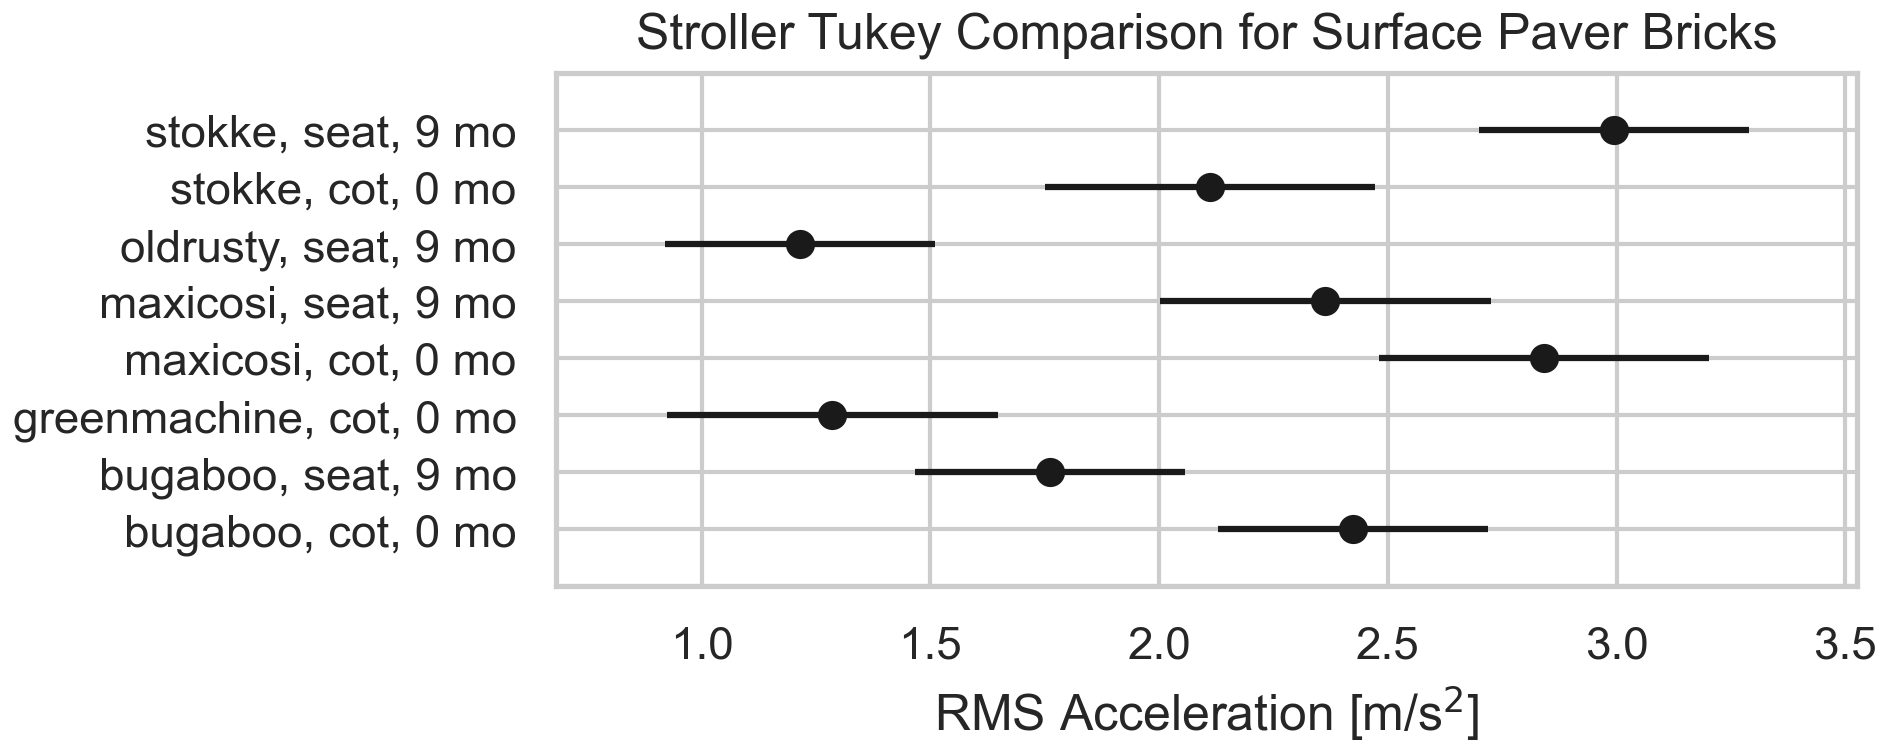
\includegraphics[width=90mm]{fig/tukey-SeatBotacc_ver-stroller-Paver Bricks.png}}
  \subcaptionbox{}{
  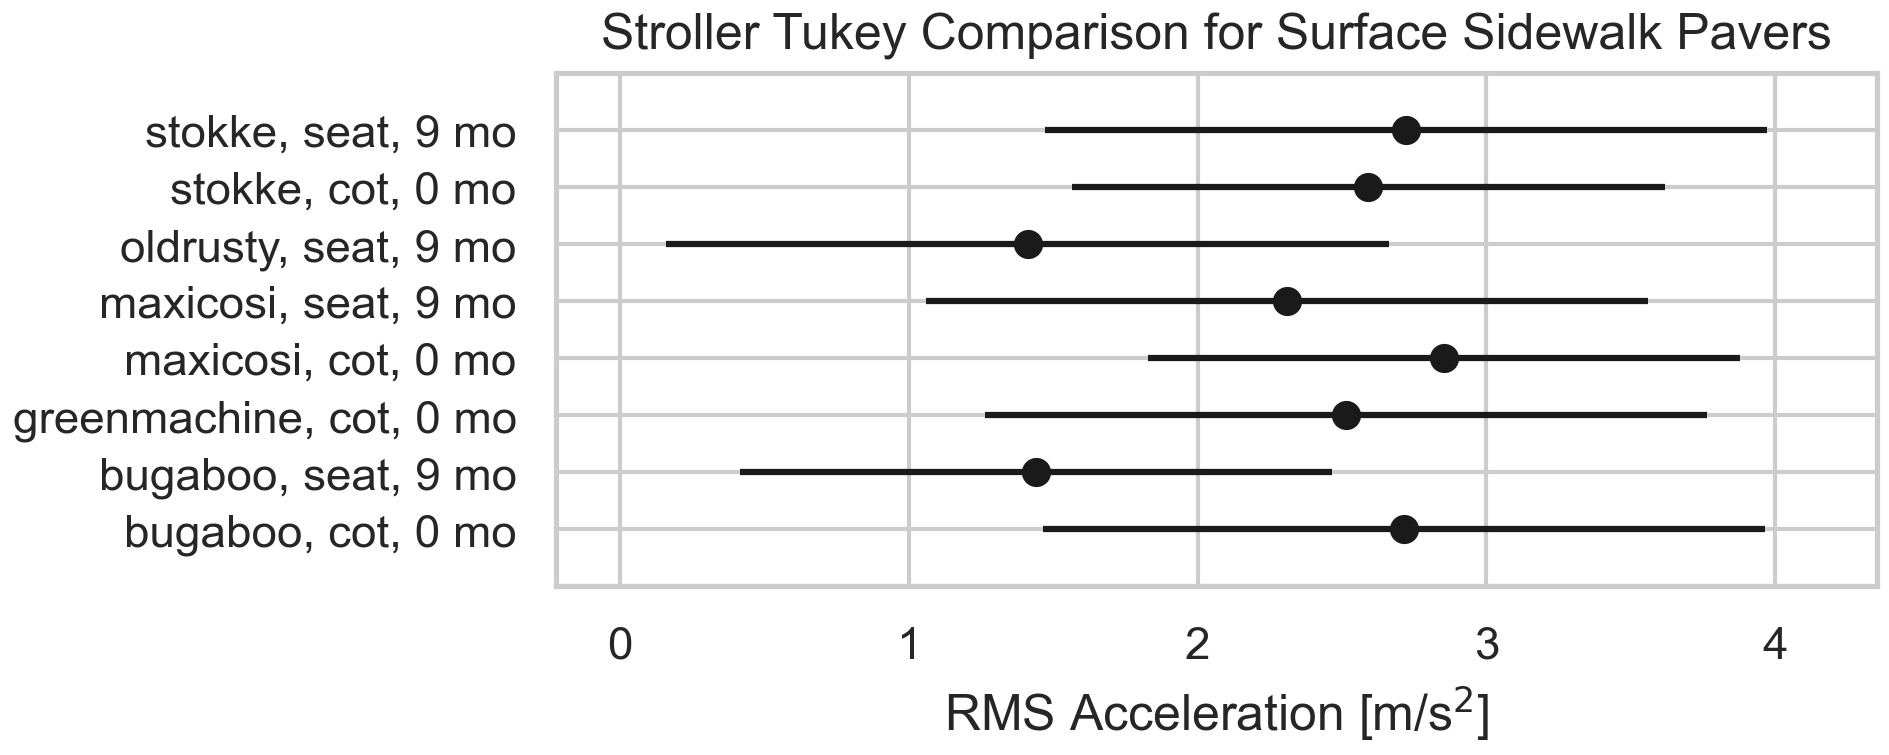
\includegraphics[width=90mm]{fig/tukey-SeatBotacc_ver-stroller-Sidewalk Pavers.png}}
  \subcaptionbox{}{
  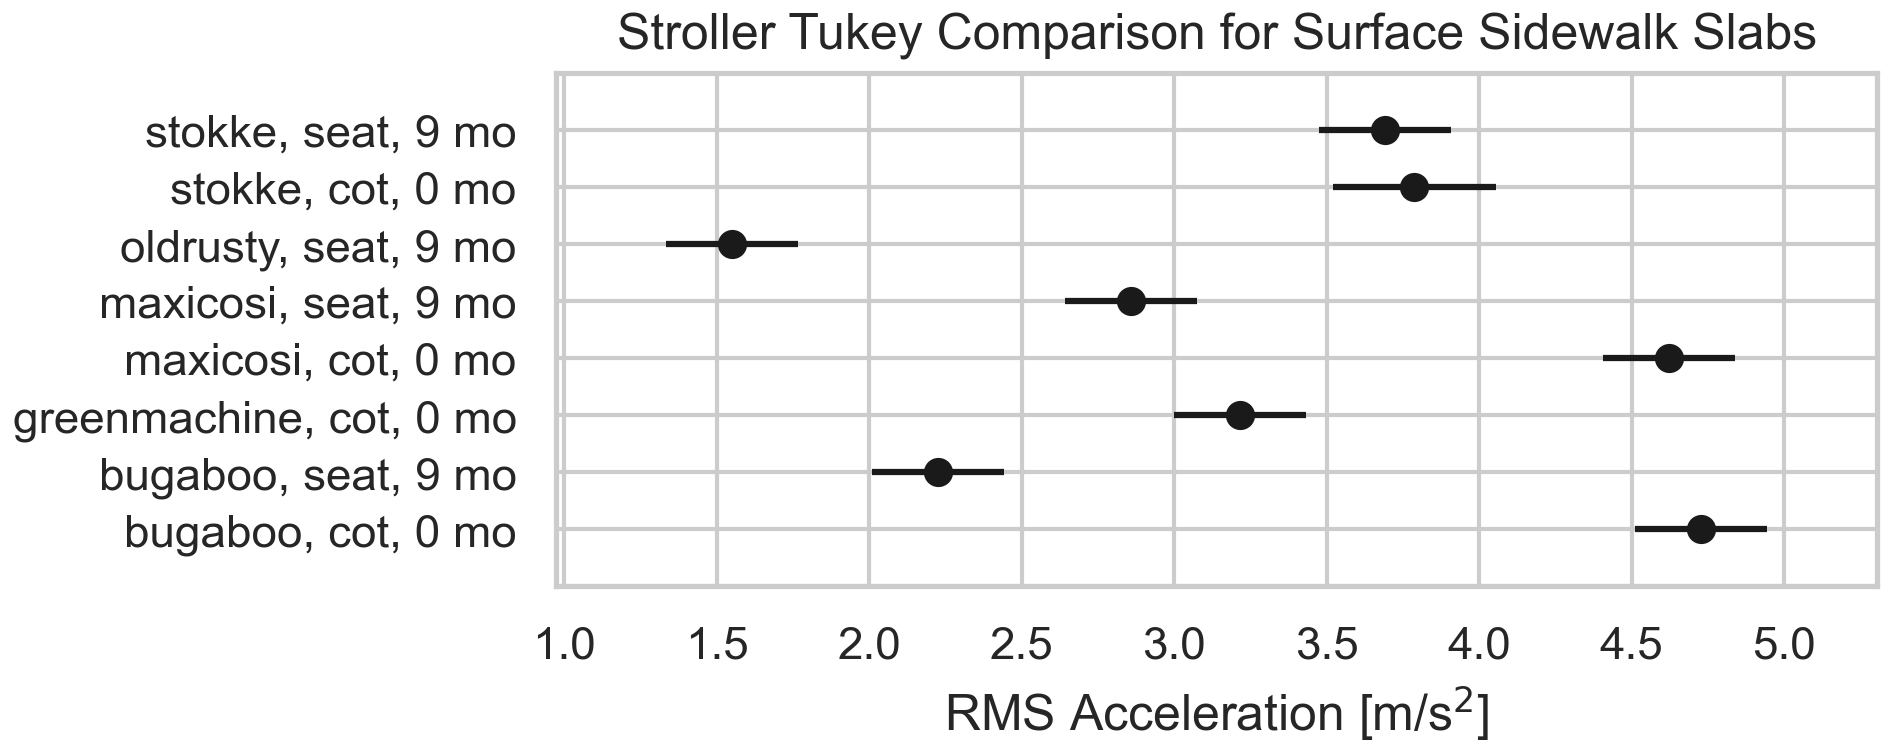
\includegraphics[width=90mm]{fig/tukey-SeatBotacc_ver-stroller-Sidewalk Slabs.png}}
  \subcaptionbox{}{
  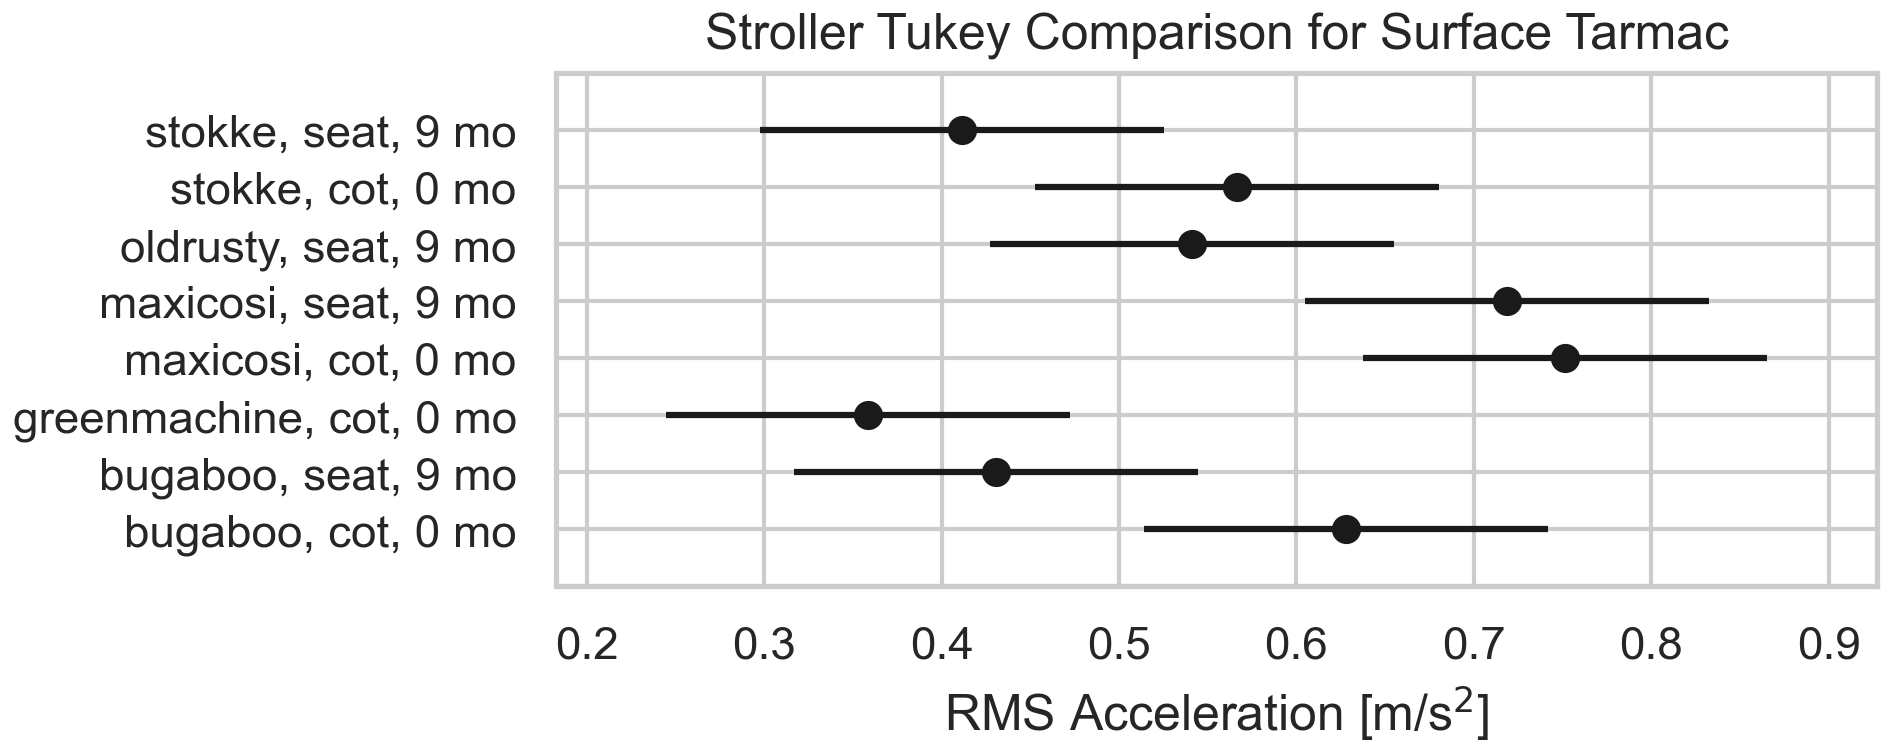
\includegraphics[width=90mm]{fig/tukey-SeatBotacc_ver-stroller-Tarmac.png}}
  \caption{Tukey Comparison Plots for the Strollers}
  \label{fig:tukey-stroller}
\end{figure}
%
\begin{figure}[!ht]
  \centering
  \subcaptionbox{}{
  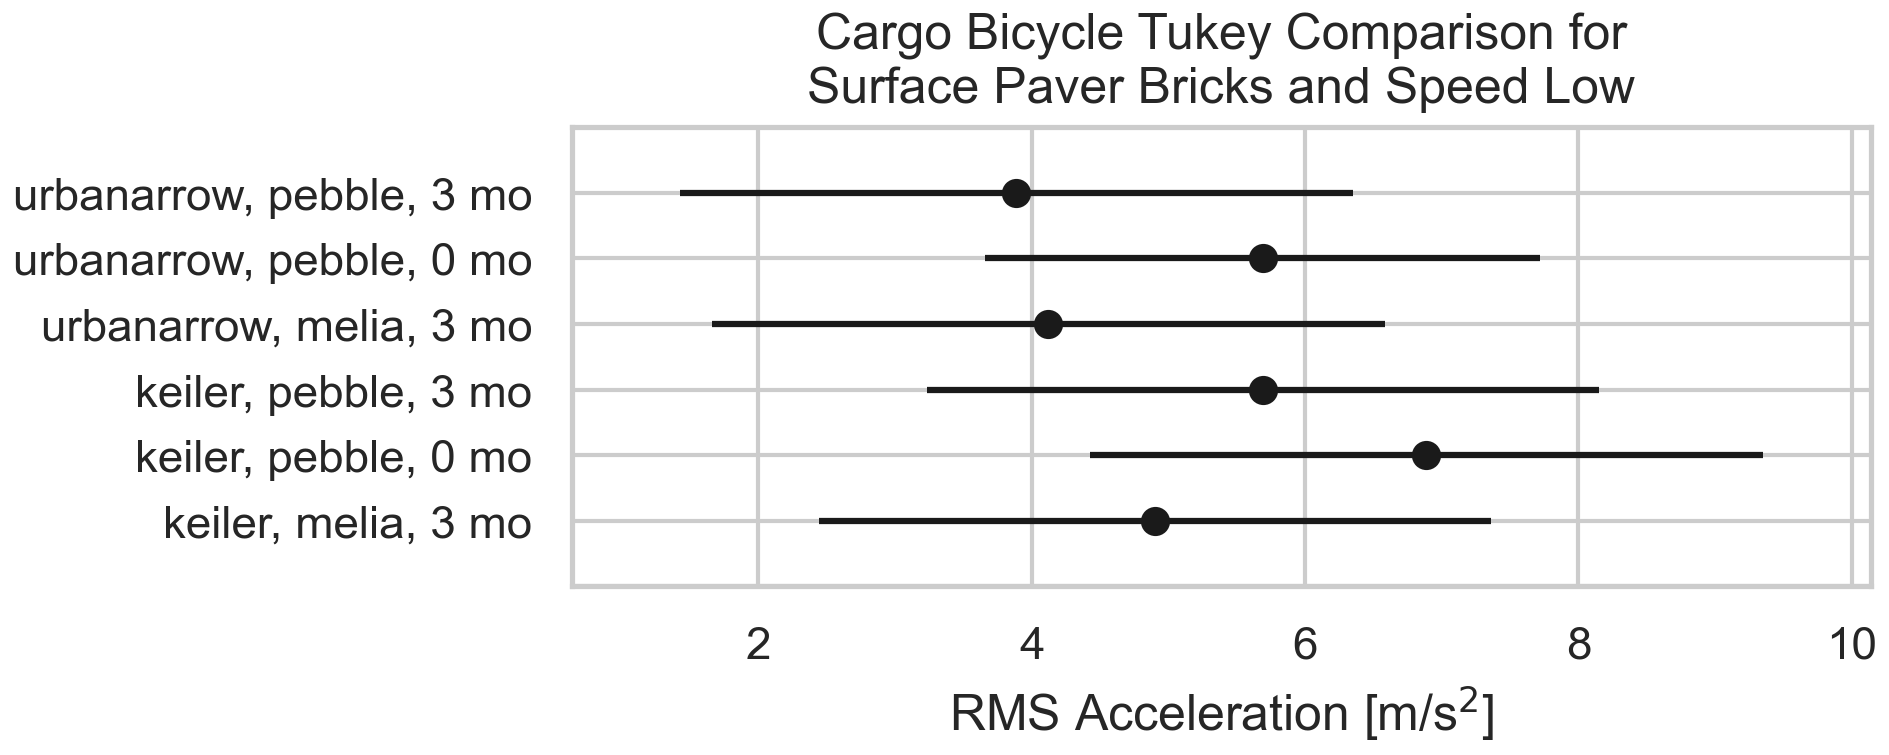
\includegraphics[width=90mm]{fig/tukey-SeatBotacc_ver-bicycle-Paver Bricks-Low.png}}
  \subcaptionbox{}{
  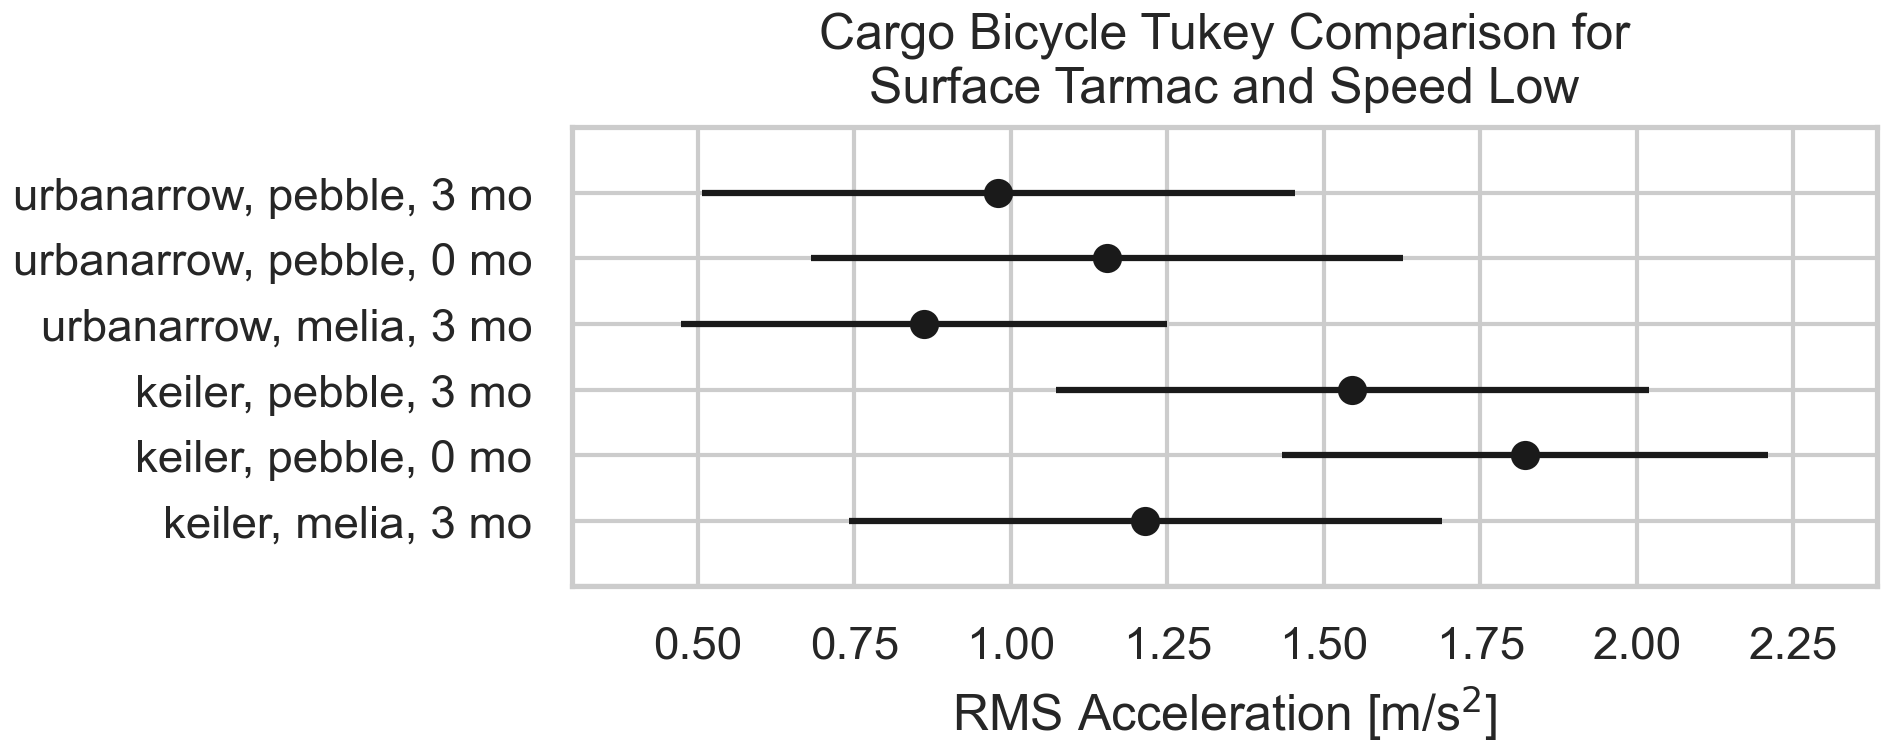
\includegraphics[width=90mm]{fig/tukey-SeatBotacc_ver-bicycle-Tarmac-Low.png}}
  \subcaptionbox{}{
  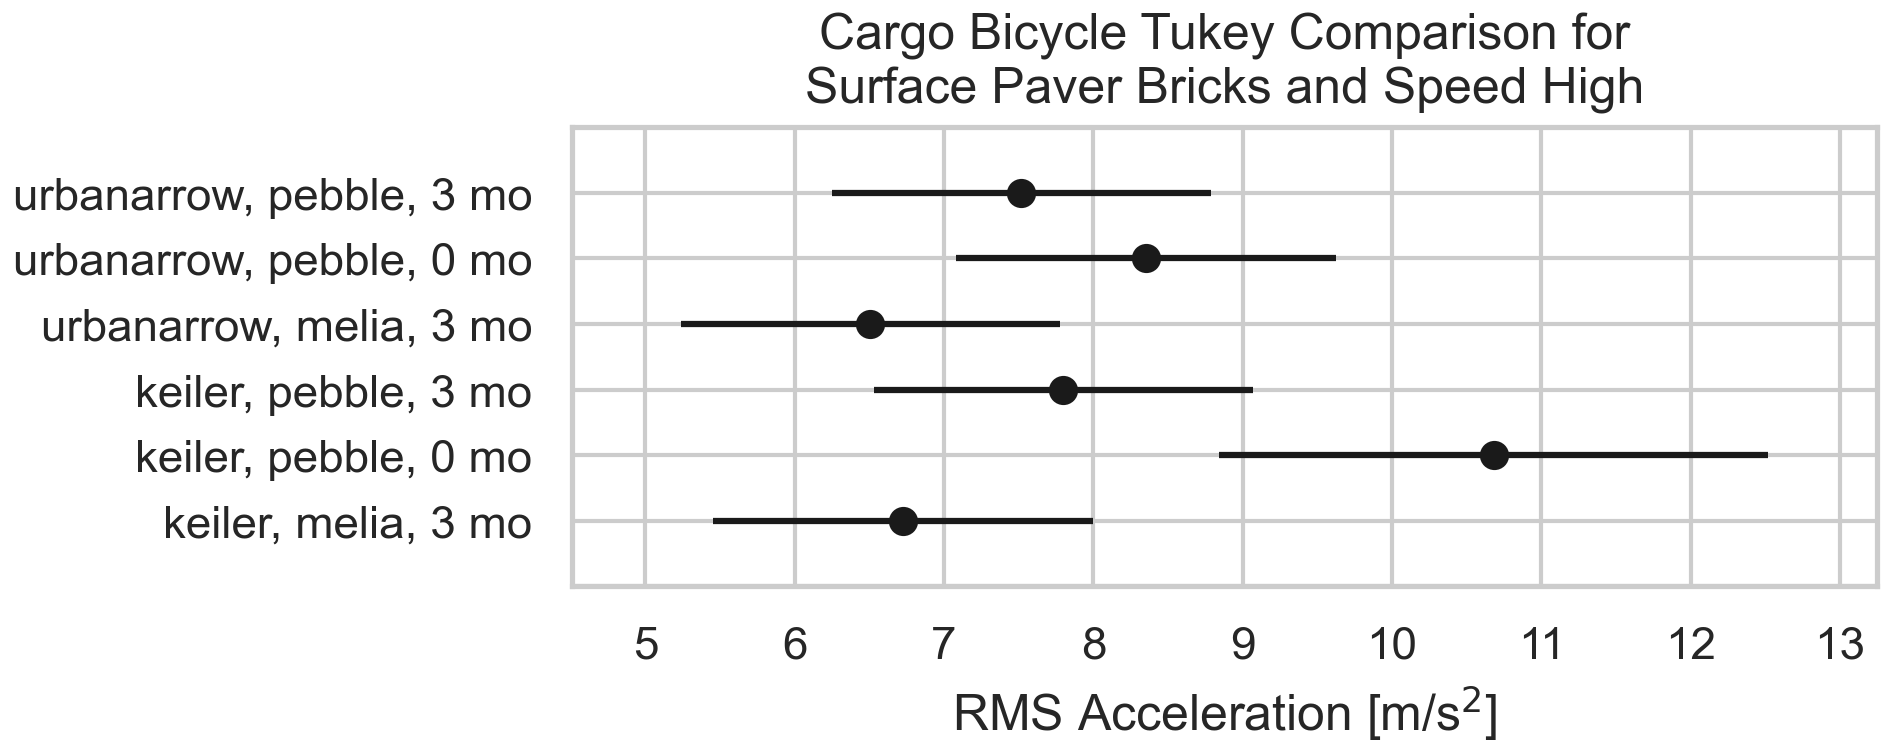
\includegraphics[width=90mm]{fig/tukey-SeatBotacc_ver-bicycle-Paver Bricks-High.png}}
  \subcaptionbox{}{
  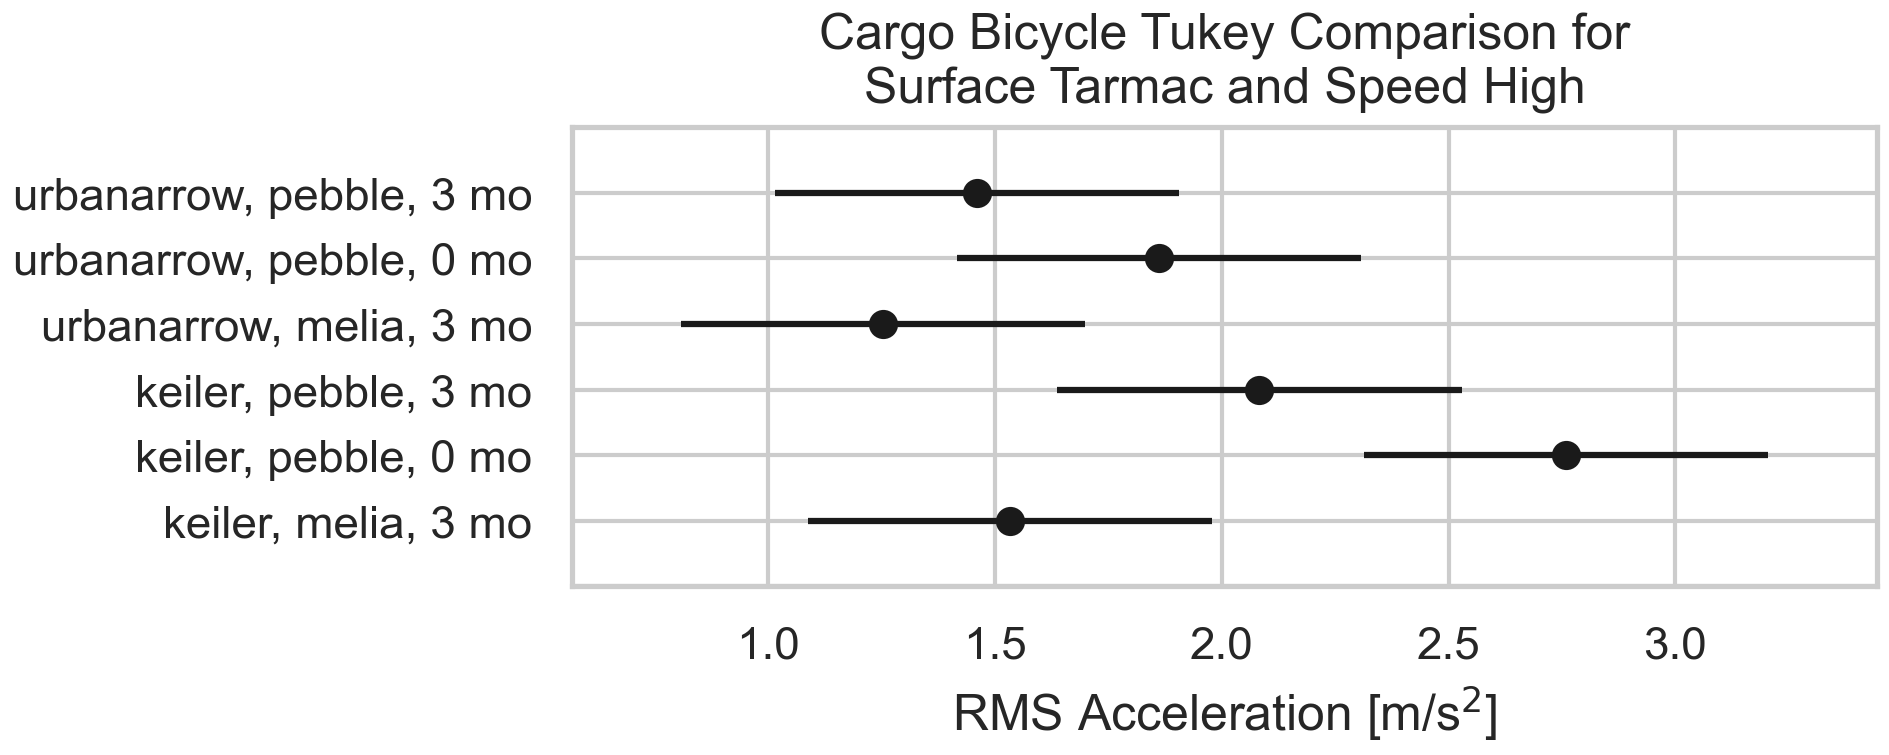
\includegraphics[width=90mm]{fig/tukey-SeatBotacc_ver-bicycle-Tarmac-High.png}}
  \caption{Tukey Comparison Plots for the Cargo Bicycles}
  \label{fig:tukey-bicycle}
\end{figure}

\newpage
\section{Shock tests}
\label{app:shock}

We identified the maximum peak acceleration values for each trial
(Equation~\ref{eq:max-acc}), then averaged them across repetitions to obtain the
results listed in Table~\ref{tab:shock} for different vehicles and
configurations. There is a significant variation between tests, with the peaks for
the bicycles sometimes reaching the full scale of the accelerometer (\(\pm\)16~g).
The seat pan accelerations for strollers are generally lower than
those experienced with bicycles, but in strollers the configuration (0 or 9 months) may play
a large role. Among bicycles, the Melia seems to transmit
lower accelerations compared to Pebble, 3 months, for both the Keiler and the Urban Arrow. Strollers with the baby seat configuration for 9
months show much lower acceleration compared to the baby cot for 0 months
(Bugaboo and Maxi-Cosi). Surprisingly, the vintage strollers (Old Rusty and Green
Machine) performed very well during the shock test, resulting in the lowest seat
pan acceleration among all the vehicles tested.
Figure~\ref{fig:shock_vehicle_comparison} shows the peaks of the vertical
acceleration recorded at the seat pan, grouped by different vehicles, for the
shock test. As noted in Table~\ref{tab:shock}, the vintage strollers Old Rusty and
Green Machine show lower acceleration values. We do not clearly distinguish any
trend with speed for the bicycles (Keiler and Urban Arrow). During tests
involving Keiler and strollers, we cannot exclude that the front wheels
(left and right) hit the bump at slightly different time instants.   

Regarding the
shock test, the analysis presented in Appendix~\ref{app:shock} was conducted on
unfiltered data (not downsampled). We selected the maximum (absolute) peak from
the time history of the vertical acceleration of the seat pan starting from the
events' time histories (Figure \ref{fig:shock_time-history}), limiting it to
16~g when the peak exceeded that maximum.

\begin{align}
  \textrm{MAX}_{a_{z}} =\max|a_{z}(t_n)|
  \label{eq:max-acc}
\end{align}

%
\begin{figure}
  \centering
  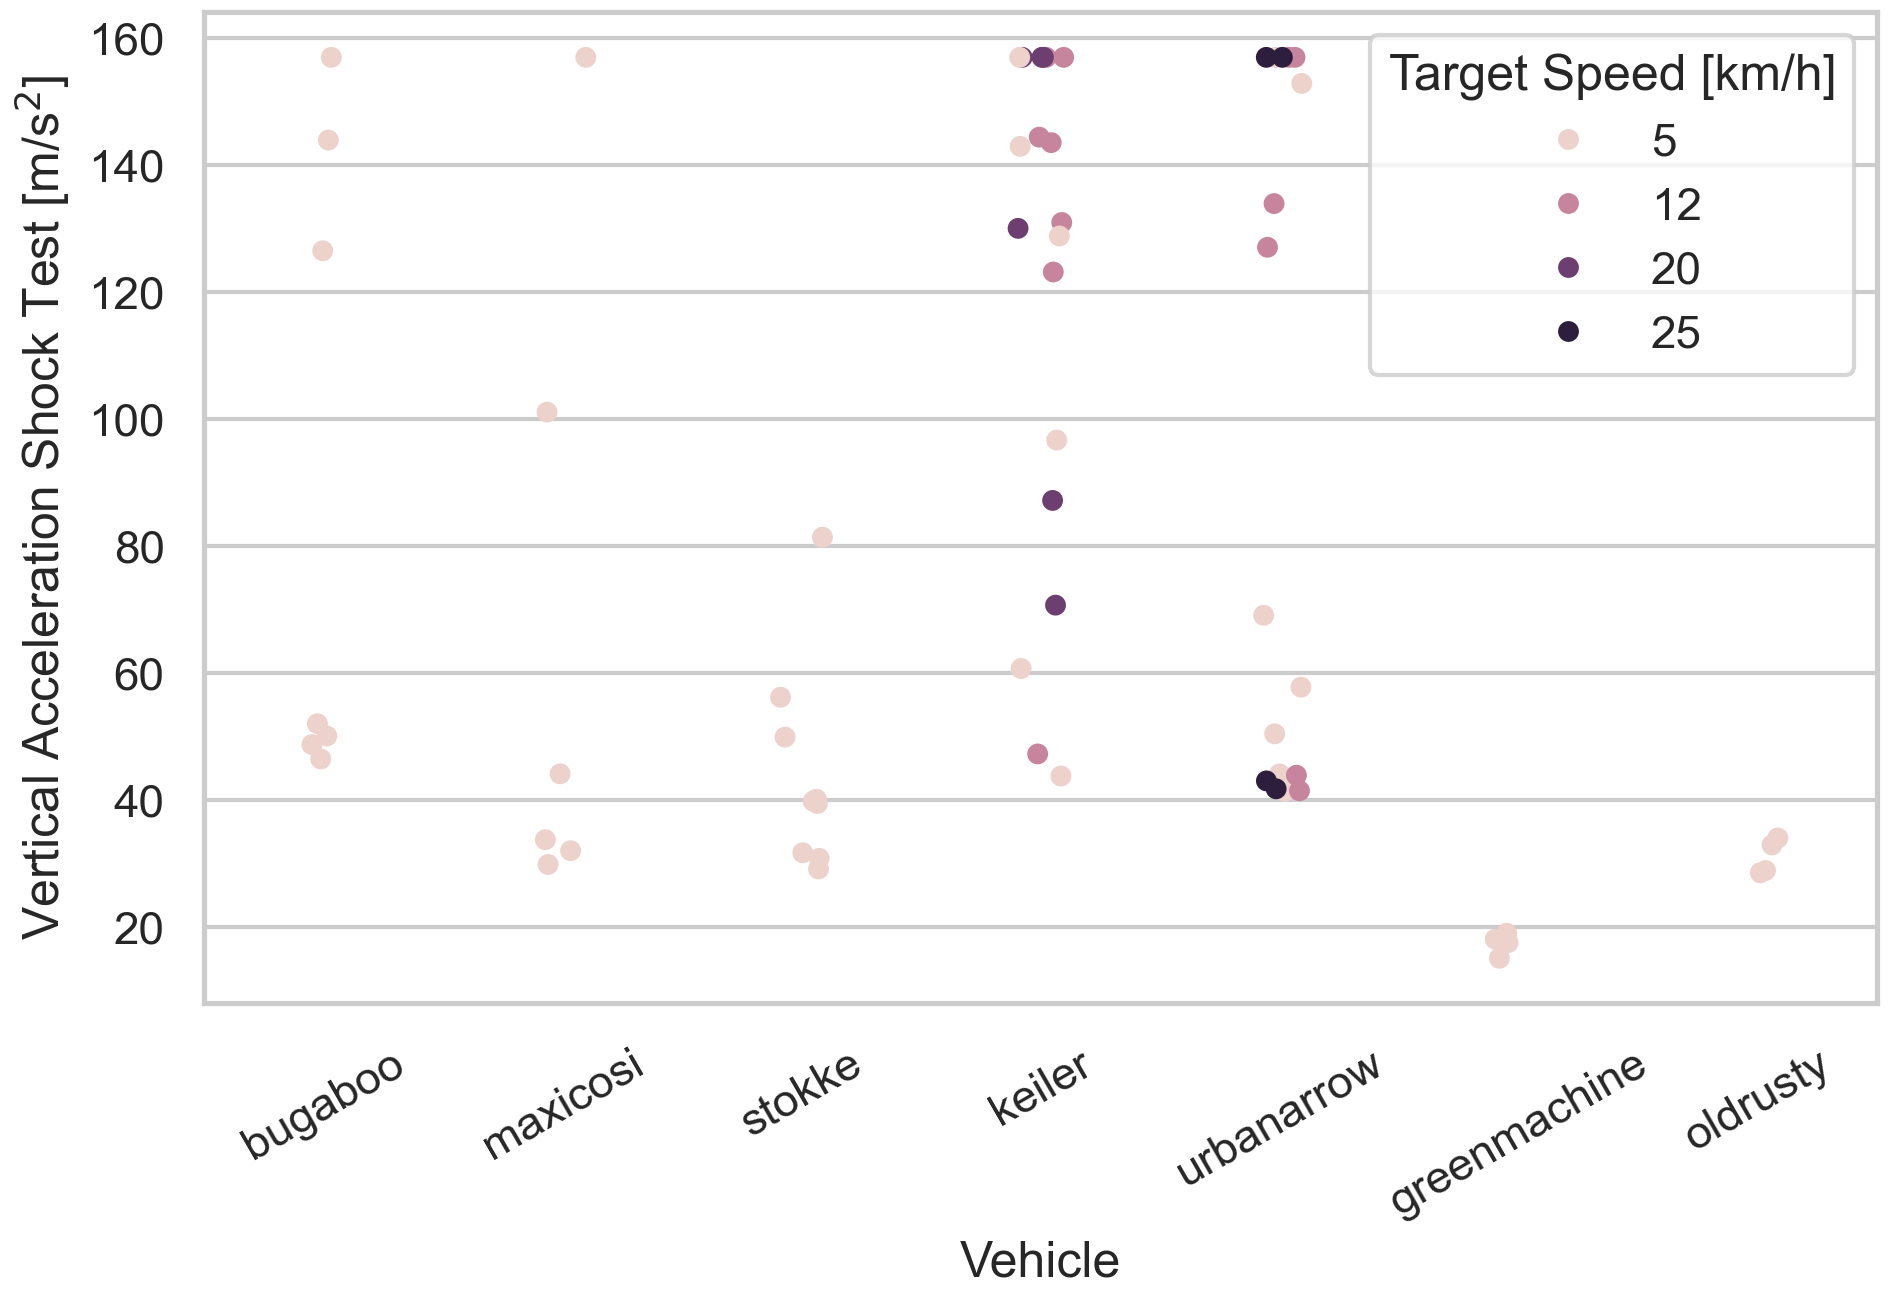
\includegraphics[width=160mm]{fig/SeatBotacc_ver-shock-test-compare.png}
  \caption{Vertical acceleration recorded at the seat pan during the shock test
  per each trial, grouped by vehicles. The colour indicates the mean speed of
  the trial. The lighter the colour the lower the speed.}
  \label{fig:shock_vehicle_comparison}
\end{figure}

\begin{figure}
  \centering
  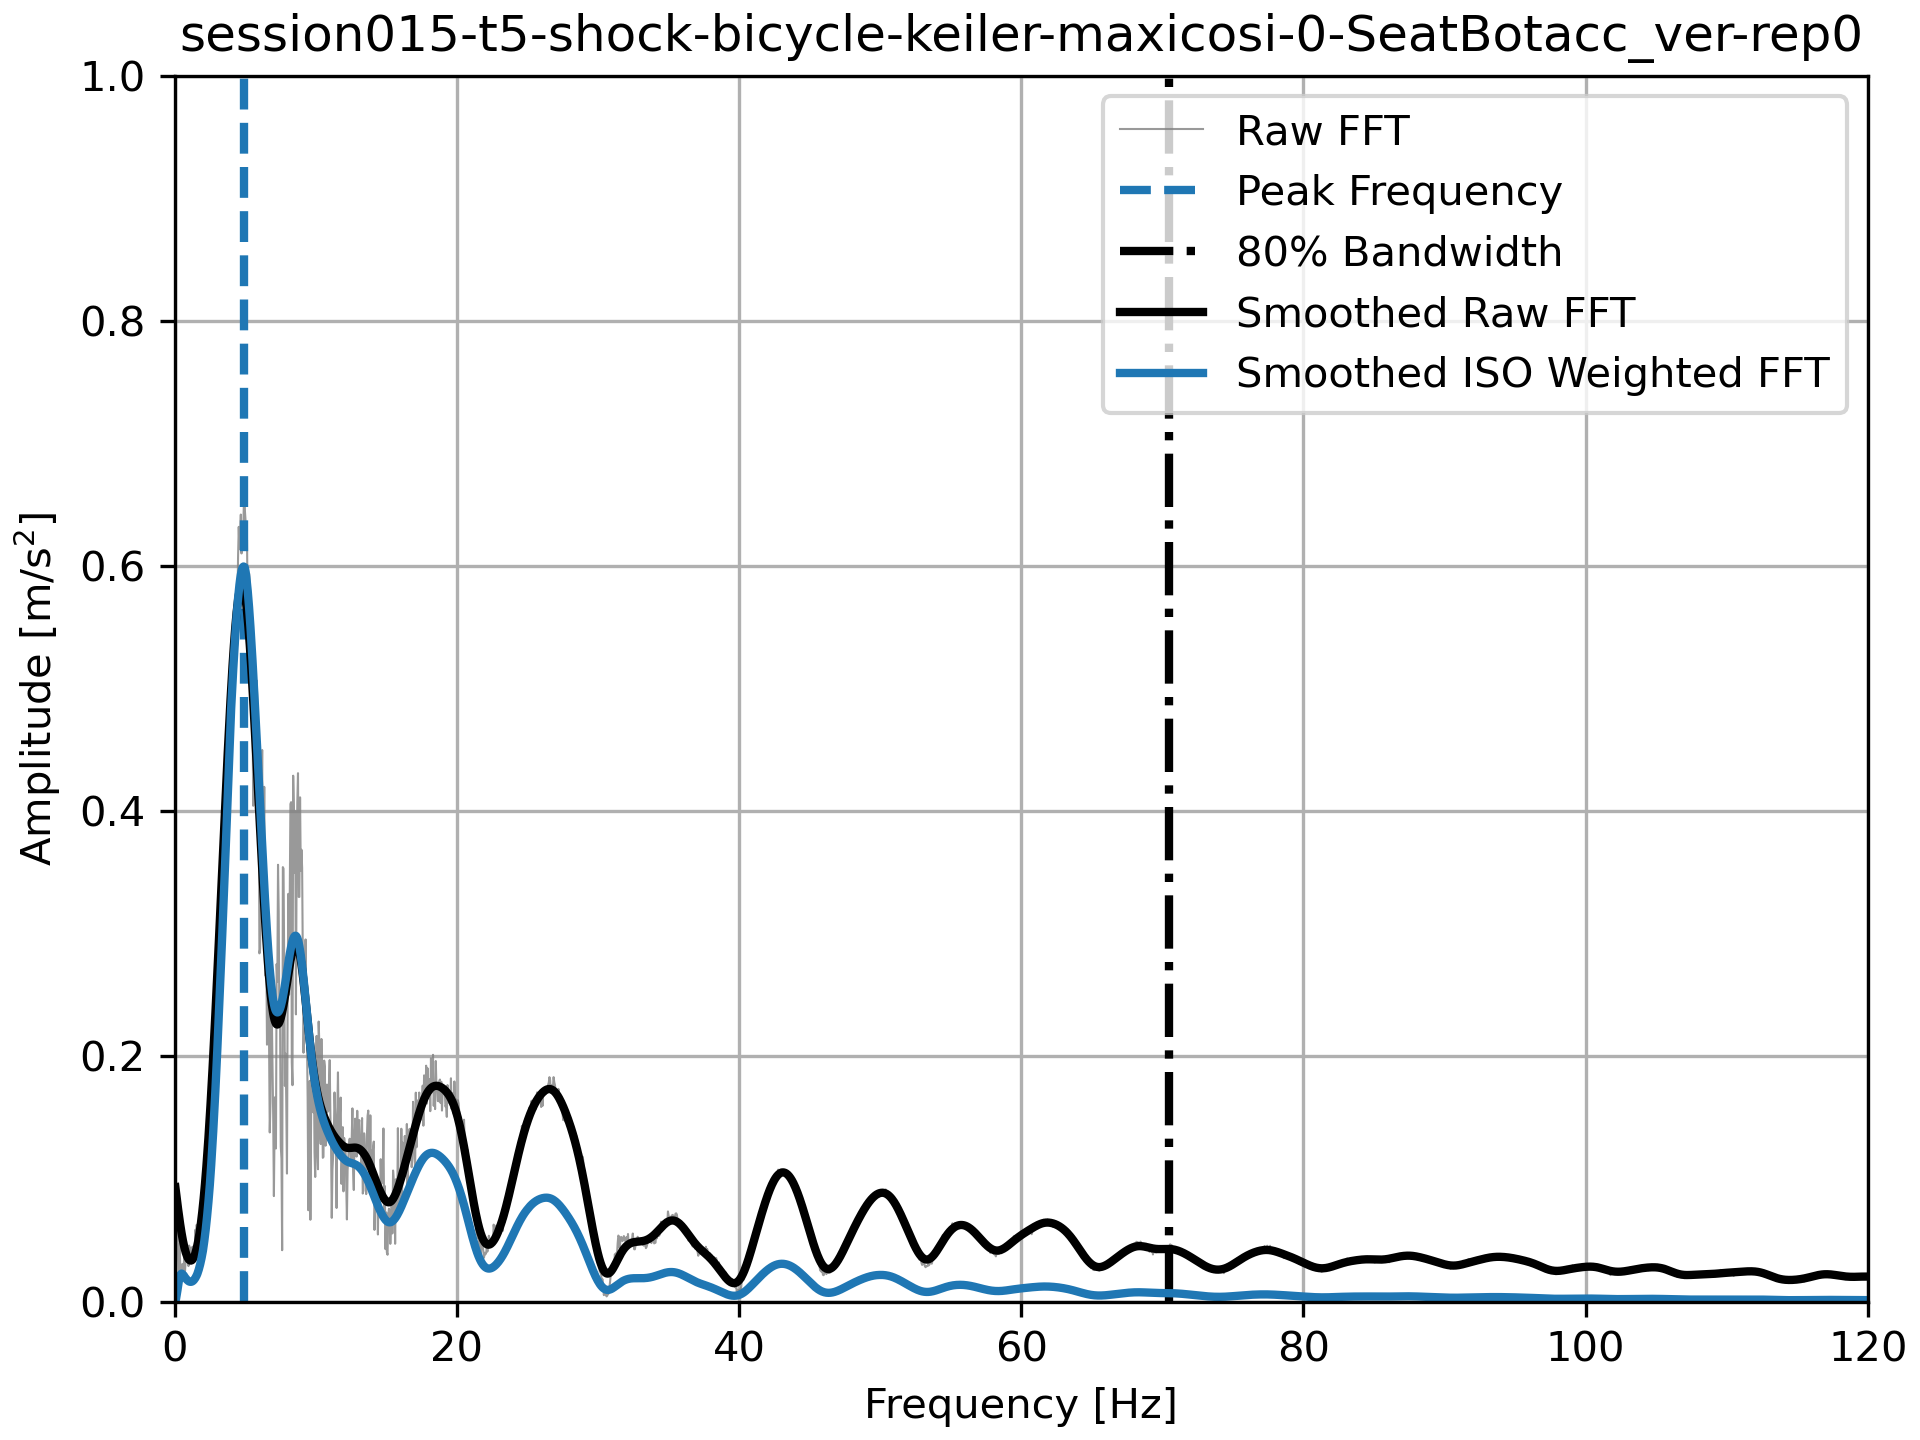
\includegraphics[width=160mm]{fig/session015-t5-shock-bicycle-keiler-maxicosi-0-SeatBotacc_ver-rep0.png}
  \caption{Raw seat pan vertical acceleration versus time from session 015:
  Keiler tricycle during the shock test.}
  \label{fig:shock_time-history}
\end{figure}

\begin{table}
  \centering
  \caption{Mean of the maximum seat pan acceleration across trials in
  \si{\mps\squared} recorded for shock test, for different vehicles and baby
  masses.}
  \label{tab:shock}
  \footnotesize
  \begin{tabular}{lllrrrr}
    \toprule
     & &  & Target Speed & Trial Count & Max Acceleration \\
    Vehicle Type & Model & Seat, Baby & [km/h] & & [m/s²] \\
    \midrule
    Strollers & Bugaboo & Cot, 0 mo  & 5 & 3 & 146 \\
              &         & Seat, 9 mo & 5 & 4 & 49 \\
    \cline{2-6}
              & Green Machine & Cot, 0 mo & 5 & 4 & 17 \\
    \cline{2-6}
              & Maxi-Cosi & Cot, 0 mo  & 5 & 2 & 131 \\
              &           & Seat, 9 mo & 5 & 4 & 35 \\
    \cline{2-6}
              & Old Rusty & Seat, 9 mo & 5 & 4 & 31 \\
    \cline{2-6}
              & Stokke & Cot, 0 mo  & 5 & 4 & 35 \\
              &                     & Seat, 9 mo & 5 & 4 & 51 \\
    \cline{1-6}
    Bicycles & Keiler & Melia, 3 mo & 5 & 2 & 52 \\

             &               & Melia, 3 mo & 12 & 2 & 85 \\

             &               & Melia, 3 mo & 20 & 2 & 124 \\
    \cline{2-6}
             &               & Pebble, 0 mo & 5 & 2 & 113 \\

             &               & Pebble, 0 mo & 12 & 2 & 140 \\

             &               & Pebble, 0 mo & 20 & 2 & 115 \\
    \cline{2-6}
             &               & Pebble, 3 mo & 5 & 2 & 151 \\

             &               & Pebble, 3 mo & 12 & 2 & 160 \\

             &               & Pebble, 3 mo & 20 & 2 & 145 \\
    \cline{2-6}
             & Urban Arrow & Melia, 3 mo & 5 & 2 & 43 \\

             &               & Melia, 3 mo & 12 & 2 & 43 \\

             &               & Melia, 3 mo & 25 & 2 & 42 \\
    \cline{2-6}
             &               & Pebble, 0 mo & 5 & 1 & 50 \\
    
             &               & Pebble, 0 mo & 12 & 2 & 63 \\
    
             &               & Pebble, 0 mo & 25 & 2 & 130 \\
    \cline{2-6}
             &               & Pebble, 3 mo & 5 & 2 & 156 \\
    
             &               & Pebble, 3 mo & 12 & 2 & 160 \\
    
             &               & Pebble, 3 mo & 25 & 2 & 160 \\
    \bottomrule
  \end{tabular}
\end{table}


\section{Future Work}
% 
There are four possible directions for future work: more in-depth analysis of
the present measurements, more research on the vibrations transmitted by infant
transport systems, more research on the effects of vibration on infants, and
development of a benchmark.

\paragraph{Concerning further analysis of the present measurements:}
%
We acquired data from four other sensors on the vehicles, each with three
accelerometer and three gyroscope time histories, for a total of 30 time
histories of possible interest. This paper provides a look into the experiments
via four metrics: ISO weighted vertical RMS acceleration, maximum acceleration,
peak frequency, and bandwidth of the seat pan sensor. The collected data can
also be used to investigate the transmissibility from sensor to sensor, as well
as rotational vibration effects. Investigating these further can give a more
complete picture of the connections to health and comfort. This work also gives
a benchmark against which new designs can be tested to show reduction in
vibration.

\paragraph{Concerning more research on vibrations generated by infant transport
systems:}
%
Some products, scenarios, and variables have not yet been investigated for their
effect on vibration. For example, running with an infant in a jogging stroller is a subject of interest as vibrations are likely to exceed health limits. Furthermore, recumbent postures in
jogging strollers are estimated to increase the vibration load on the head of the
infant. It is important to establish the actual vibration load on the head in
practice.

\paragraph{Concerning more research on the effects of vibration on infants:}
%
The frequency weighting of the ISO~2631-1 standard is not designed or validated
to characterise health and comfort for infants or children, for short durations,
and for non-erect seating. Research is urgently needed to develop a new standard
with a more appropriate frequency weighting to improve assessment of the comfort
and health effects of whole-body vibration of infants and children, also for
short durations and for non-erect seating. Furthermore, tests with more
realistic dummies and/or real infants are necessary to investigate how the
infant itself moves when excited by various vibrations in different postures.
The results will contribute to the assessment of the transmissibility of
vibration in children, which is needed to deduce the vibrations transmitted to
the head. 

\paragraph{Concerning the development of a benchmark:}
%
At this moment, no requirements exist for the vibrational properties of child
transport systems in the standards for strollers, cargo bicycles, bicycle seats,
bicycle trailers, and car seats. Due to the magnitude of vibrations that can
occur during child transport, it is imperative to include requirements for the
vibrational properties in the standards for these products. At this moment, it
is difficult to develop new requirements because there is not enough
information. With the information resulting from more research on infant
vibration, a benchmark for the vibration properties of infant transportation
products needs to be developed. Tests as performed in this study mark a first
milestone. Road surfaces, speeds, dummies, posture, and metrics could be
standardised. Over the years, these could be refined building upon scientific
research. Acceptance thresholds could be set to accept current products that
perform well.  This will enable the inclusion of (minimal) requirements for
vibration properties in the standards, which would greatly increase the health
and comfort of infants who must use these products. 

\section{Experimental Equipment}
\label{app:equipment}

We considered the use of ``crash test dummies'' (also known as anthropomorphic
test devices or ATDs), which are designed and commonly used to test child seats
in car crash tests. However, the closest available body sizes for crash test
dummies do not meet the body sizes desired for this investigation. Furthermore, crash test dummies are of a fundamentally different design, based on scaling of adult biomechanical data rather than child data and with dynamic properties designed for crash conditions, not for vibration testing. Therefore, crash test dummies were not used for the envisaged vibration tests. 
 The following lists the dummies used:
%
\begin{description}
  \item[Dummy 0 months] weight 3.48~\si{\kg}, size 50~\si{\cm}. Dollkit 20'',
  ``Andi Asleep'' (product code AW380008).
  (\href{http://www.atelier-wiesje.nl/index.php?item=9912---dollkit-20-_-andi-asleep--_-armen-_-_-benen----available&action=article&group_id=10000164&aid=2163&lang=NL}{Webpage})
  
  \item[Dummy 3 months] weight 5.90~\si{\kg}, size 62.5~\si{\cm}. Dollkit 25'',
  ``Asia - Limited Edition'' (product code 300287).
  (\href{http://www.atelier-wiesje.nl/index.php?action=article&aid=2556&group_id=10000176&lang=NL}{Webpage})
  \item[Dummy 9 months] weight 8.90~\si{\kg}, size 70~\si{\cm}. Dollkit 28'',
  ``Hailey'' (product code 304137).
  (\href{http://www.atelier-wiesje.nl/index.php?action=article&aid=1974&group_id=10000133&lang=NL}{Webpage})
\end{description}
%
The strollers and bicycles used for the experiments are shown below, along with their wheelbase, wheel diameter, sensor location, and orientation for all the tested vehicles.

\begin{description}
\item[Strollers] A selection of vintage and modern strollers for carrying
infants. The modern strollers are configurable as cots for newborns and as seats
for older infants.
%
\begin{description}
  \item[Bugaboo Fox 5] Featuring large wheels and a suspension system that makes
  it an all-terrain stroller, according to the manufacturer. It has large
  puncture-resistant tyres and an air-permeable mattress.
  (\href{https://www.bugaboo.com/nl-nl/speciale-aanbiedingen/bugaboo-fox-5-bassinet-and-seat-stroller-black-base-midnight-black-fabrics-midnight-black-sun-canopy-PV006272.html?gad_source=1&gclid=Cj0KCQiA1Km7BhC9ARIsAFZfEIuB-6fQPRl5KyIHVJtion5lyD_Z1Qn-IP3shWoB_HXFozM1ySTXNfgaAgzFEALw_wcB&gclsrc=aw.ds}{Bugaboo
  website})
  \item[Green Machine] An unknown brand vintage perambulator with a cot, dating
  approximately from the 1970s that includes a leather strap suspended cot in a
  metal frame. The wheels are relatively large compared to modern strollers.
  \item[Maxi-Cosi Street Plus] This stroller comes with a cot configuration (0-6
  months) and an infant seat option. It has large wheels with only a marginal suspension system.
  (\href{https://www.maxi-cosi.nl/kinderwagens/street-plus?color_swatch_id=5519}{Maxi-Cosi website})
  \item[Old Rusty] An unknown brand vintage seat-style stroller dating approximately from the 1970s that includes a metal spring suspension system and wheels that are slightly larger than those on modern strollers.
  \item[Stokke BABYZEN YOYO 0+] Among the smallest foldable strollers on the market. It has only a marginal suspension system and smaller wheels compared to other strollers available on the market.
  (\href{https://tinylibrary.nl/products/kinderwagen-babyzen-yoyo-0-plus}{Model
  rented for the experiment})
\end{description}
\item[Cargo Bicycles] Two modern Dutch ``bakfietsen'' in which different baby
seats can be mounted.
%
\begin{description}
  \item[Keiler Tricycle] A tadpole (two wheels in the front, one in the rear)
  cargo tricycle without electric assist. This vehicle will not roll into
  curves. However, differing road surface unevenness at the left and right front
  wheels will induce lateral roll and lateral acceleration in infants. We added
  masses in specific locations to simulate the presence of an electric motor and
  battery package, in order to compare the results with those of the Urban
  Arrow. The tricycle was equipped with tyres CST XPEDIUM Safe 47-559
  (Cheng Shin Tire, Yuanlin, Taiwan) on the rear, and Schwalbe Green Comfort Road Cruiser
  K-Guard 3 47-507 (Ralf Bohle GmbH, Reichshof-Wehnrath, Germany) on
  the front. We set both tyres to an inflation pressure of 300~\si{\kPa}.
  (\href{https://kashop.nl/product/keiler-bakfiets/}{Product Webpage}) 
  \item[Urban Arrow Cargo Bicycle] An electric cargo bicycle that is popular in
  the Netherlands. This vehicle has two inline wheels, which makes it roll into
  curves like a regular bicycle. It is featured by a long frame that can carry
  loads (e.g., a child in a car seat or a baby shell) placed in between the
  rider and the front wheel. We used the ''Family Performance Plus'' model, with
  an electric drivetrain from Bosch Performance Line (65~\si{\N}\si{\m},
  250~\si{\W}). It was equipped with tyres Schwalbe Big Ben Plus 55-559 on the
  rear, and Schwalbe Big Ben Plus 55-406 on the front (Ralf Bohle GmbH, Reichshof-Wehnrath, Germany). We set both tyres to an
  inflation pressure of 300~\si{\kPa}, according to the range recommended by the
  manufacturer.
  (\href{https://urban arrow.com/}{Urban Arrow website})
\end{description}
\item[Baby Seats] These two baby seats were mounted in the cargo bays of the two
cargo bicycles.
%
\begin{description}
  \item[Melia Baby Shell] Baby seat specifically designed for cargo bicycles
  meant for babies from 2 to 9 months old. Mounted to the seat platform in both
  cargo bicycles.
    (\href{https://melia.nl/product/babyschaal-4-seizoenen-comfort/}{Melia
    Webpage})
  \item[Maxi-Cosi X Joolz Pebble Pro i-Size Car Seat] Can be adapted to be
  mounted on cargo bicycles with a fitting fixing system (e.g. ``Urban Arrow
  Baby Car Seat Adapter''). Comes with an integrated suspension system. The same
  adapter was used in both cargo bicycles.
    (\href{https://www.maxi-cosi.nl/autostoelen/pebble-pro-i-size}{Maxi-Cosi
    Webpage})
\end{description}
\end{description}

Additional sensor locations are as follows.

\begin{enumerate}
  \item \textbf{Front Wheel} This IMU was mounted on the front wheel fork (the
  caster wheel for the stroller). This was the non-rotating measurement point
  closest to the ground. The purpose of this sensor was to measure the road
  roughness filtered out only by the tyres.  
  \item \textbf{Frame} On the cargo bicycle, an IMU was placed below the frontal
  cargo bay and clamped to the frame. This was to provide an understanding of
  the damping characteristics of the bicycle frame, together with an estimation
  of the effect of the suspension system. On the stroller, the IMU was taped
  under the baby seat.
  \item \textbf{Seat Head} IMU taped into the baby seat (on the soft mattress),
  directly in contact with the dummy's head. This IMU measured the vibration
  transmitted to the head contact point.
\end{enumerate}

\begin{figure}
  \centering
  \subcaptionbox{IMU on the front fork}{\includegraphics[width=0.45\textwidth, angle=-90]{fig/FW_UA.jpg}}
  \subcaptionbox{IMU under the cargo bay}{\includegraphics[width=0.45\textwidth, angle=-90]{fig/BT_UA.jpg}}
  \caption{IMU locations on the Urban Arrow. The white 3D printed
  sensor supports are visible in (a) and (c). The last figure (d) shows how the
  sensors were taped to the seat pan and backrest.}
  \label{fig:sensors_UA2}
\end{figure}

\begin{figure}[htbp]    % use [htbp] to place the figures where I prefer
  \centering
  \subcaptionbox{Lateral view}{\includegraphics[width=75mm]{fig/TechDraw_UA-Joolz_lat.pdf}}
  \subcaptionbox{Front view}{\includegraphics[width=80mm]{fig/TechDraw_UA-Joolz_front.pdf}}
  \caption{IMU locations on the Urban Arrow, equipped with
  Pebble.}
  \label{fig:tech_drawing_UA_Joolz}
\end{figure}

\begin{figure}[htbp]    % use [htbp] to place the figures where I prefer
  \centering
  \subcaptionbox{Lateral view}{\includegraphics[width=75mm]{fig/TechDraw_UA-Melia_lat.pdf}}
  \subcaptionbox{Front view}{\includegraphics[width=80mm]{fig/TechDraw_UA-Melia_front.pdf}}
  \caption{IMU locations on the Urban Arrow, equipped with
  Melia.}
  \label{fig:tech_drawing_UA_Melia}
\end{figure}

\clearpage
\begin{figure}[htbp]
  \centering
  \subcaptionbox{Lateral view}{\includegraphics[width=75mm]{fig/TechDraw_Trike-Joolz_lat.pdf}}
  \subcaptionbox{Front view}{\includegraphics[width=80mm]{fig/TechDraw_Trike-Joolz_front.pdf}}
  \caption{IMU locations on the Keiler, equipped with
  Pebble.}
  \label{fig:tech_drawing_Trike_Joolz}
\end{figure}


\begin{figure}[htbp]
  \centering
  \subcaptionbox{Lateral view}{\includegraphics[width=75mm]{fig/TechDraw_Trike-Melia_lat.pdf}}
  \subcaptionbox{Front view}{\includegraphics[width=75mm]{fig/TechDraw_Trike-Melia_front.pdf}}
  \caption{IMU locations on the Keiler, equipped with
  Melia.}
  \label{fig:tech_drawing_Trike_Melia}
\end{figure}

\clearpage
\begin{figure}[htbp]
  \centering
  \subcaptionbox{Lateral view}{\includegraphics[width=70mm]{fig/TechDraw_Bugaboo0_lat.pdf}}
  \subcaptionbox{Front view}{\includegraphics[width=70mm]{fig/TechDraw_Bugaboo0_front.pdf}}
  \caption{IMU locations on the Bugaboo, configured for a 0-month-old baby.}
  \label{fig:tech_drawing_Bugaboo0}
\end{figure}

\begin{figure}[htbp]
  \centering
  \subcaptionbox{Lateral view}{\includegraphics[width=70mm, angle=-90]{fig/TechDraw_Bugaboo9_lat.pdf}}
  \subcaptionbox{Front view}{\includegraphics[width=70mm]{fig/TechDraw_Bugaboo9_front.pdf}}
  \caption{IMU locations on the Bugaboo, configured for a 9-month-old baby.}
  \label{fig:tech_drawing_Bugaboo9}
\end{figure}

\clearpage
\begin{figure}[htbp]
  \centering
  \subcaptionbox{Lateral view}{\includegraphics[width=70mm, angle=-90]{fig/TechDraw_Maxicosi0_lat.pdf}}
  \subcaptionbox{Front view}{\includegraphics[width=70mm]{fig/TechDraw_Maxicosi0_front.pdf}}
  \caption{IMU locations on the Maxi-Cosi, configured for a 0-month-old baby.}
  \label{fig:tech_drawing_Maxicosi0}
\end{figure}

\begin{figure}[htbp]
  \centering
  \subcaptionbox{Lateral view}{\includegraphics[width=70mm, angle=-90]{fig/TechDraw_Maxicosi9_lat.pdf}}
  \subcaptionbox{Front view}{\includegraphics[width=70mm,angle=-90]{fig/TechDraw_Maxicosi9_front.pdf}}
  \caption{IMU locations on the Maxi-Cosi, configured for a 9-month-old baby.}
  \label{fig:tech_drawing_Maxicosi9}
\end{figure}

\clearpage
\begin{figure}[htbp]
  \centering
  \subcaptionbox{Lateral view}{\includegraphics[width=70mm, angle=-90]{fig/TechDraw_YOYO0_lat.pdf}}
  \subcaptionbox{Front view}{\includegraphics[width=70mm]{fig/TechDraw_YOYO0_front.pdf}}
  \caption{IMU locations on the Stokke, configured for a 0-month-old baby.}
  \label{fig:tech_drawing_YOYO0}
\end{figure}

\begin{figure}[htbp]
  \centering
  \subcaptionbox{Lateral view}{\includegraphics[width=70mm, angle=-90]{fig/TechDraw_YOYO9_lat.pdf}}
  \subcaptionbox{Front view}{\includegraphics[width=70mm]{fig/TechDraw_YOYO9_front.pdf}}
  \caption{IMU locations on the Stokke, configured for a 9-month-old baby.}
  \label{fig:tech_drawing_YOYO9}
\end{figure}

\clearpage
\begin{figure}[htbp]
  \centering
  \subcaptionbox{Lateral view}{\includegraphics[width=70mm, angle=-90]{fig/TechDraw_GreenM0_lat.pdf}}
  \subcaptionbox{Front view}{\includegraphics[width=70mm]{fig/TechDraw_GreenM0_front.pdf}}
  \caption{IMU locations on the Green Machine, configured for a 0-month-old baby.}
  \label{fig:tech_drawing_GreenM0}
\end{figure}

\begin{figure}[htbp]
  \centering
  \subcaptionbox{Lateral view}{\includegraphics[width=70mm, angle=-90]{fig/TechDraw_OldR9_lat.pdf}}
  \subcaptionbox{Front view}{\includegraphics[width=70mm]{fig/TechDraw_OldR9_front.pdf}}
  \caption{IMU locations on the Old Rusty, configured for a 9-month-old baby.}
  \label{fig:tech_drawing_OldR9}
\end{figure}

\clearpage
\newpage

\section{Location and pictures of the experiment areas}
\label{app:location}
%
\begin{itemize}
  \item \textbf{Strollers} were tested with dummies of 0 months and 9 months at
  5~\si{\kph} at:
  \begin{itemize}
      \item Tarmac
      \item Paver bricks % Klinkers
      \item Sidewalk pavers % Stoeptegels
      \item Cobblestones 
      \item Sidewalk slabs (concrete blocks with gaps in between) % Aula blocks
      \item Shock bump: A 30x30~\si{\mm} square section aluminium bar 
  \end{itemize}
  \item \textbf{Cargo bicycles} were tested with dummies of 0 months and 3
  months. Tests were performed at 12~\si{\kph} for both vehicles. The Urban Arrow
  was also tested at 25~\si{\kph} whereas the Keiler was tested at
  20~\si{\km\per\hour} for safety reasons (due to wobbling). The test surfaces
  are:
  \begin{itemize}
      \item Tarmac
      \item Paver bricks
      \item Shock bump: A 30~\si{\mm} x 30~\si{\mm} square section aluminium bar (also tested at 5~\si{\kph})
      \end{itemize}
  \item \textbf{Baby seats} Both the Pebble and the
  Melia was tested on each cargo bicycle using the same mounting
  systems.
\end{itemize}

\subsection{For Bicycles}

\begin{itemize}
    \item Tarmac
\begin{figure}[htbp]
  \centering
  {\includegraphics[width=70mm, angle=-90]{fig/Tarmac_bicycle.pdf}}
  \caption{Tarmac surface where we tested bicycles.}
  \label{fig:tarmac_bicycle}
\end{figure}

The bicycle experiment on the tarmac was conducted along Leeghwaterstraat, 2628 CA Delft, The Netherlands (GPS coordinates: 52.001053, 4.369071).

    \item Paver bricks
\begin{figure}[htbp]
  \centering
 {\includegraphics[width=70mm, angle=-90]{fig/Paver_bricks_bicycle.pdf}}
  \caption{Paver bricks surface where we tested bicycles.}
  \label{fig:paver_bricks_bicycle}
\end{figure}

The bicycle experiment on the paver bricks was conducted along Hertog Govertkade and Kanaalweg, 2611 DD Delft, The Netherlands (GPS coordinates: 52.006264, 4.363013).\\
Details of paver brick: rectangular shape, dimensions 195x95~\si{\mm} (gap in between: 7±2~\si{\mm}).

\clearpage

    \item Shock
\begin{figure}[htbp]
  \centering
  \includegraphics[width=70mm, angle=0]{fig/Shock_bicycle.pdf}
  \caption{We performed a shock test with bicycles riding over a 30x30~\si{\mm} square section bar.}
  \label{fig:shock_bicycle}
\end{figure}

The bicycle shock experiment was conducted along Leeghwaterstraat, 2628 CA Delft, The Netherlands (same location of the experiment on the tarmac, GPS coordinates: 52.001053, 4.369071).\\
Details of the shock experiment: we rode over a square-sectioned aluminium bar 30x30~\si{\mm}.

\end{itemize}

\subsection{For Strollers}

\begin{itemize}
    \item Tarmac

\begin{figure}[htbp]
  \centering
    \includegraphics[width=70mm, angle=-90]{fig/Tarmac_stroller.pdf}
  \caption{Tarmac test area.}
  \label{fig:tarmac_stroller}
\end{figure}

The bicycle experiment on the tarmac was conducted along Julianalaan, 2628 BG Delft, The Netherlands (GPS coordinates: 52.002727, 4.366845).

\clearpage

    \item Cobblestone

\begin{figure}[htbp]
  \centering
  \includegraphics[width=60mm, angle=-90]{fig/Cobblestone_stroller.pdf}
  \caption{Cobblestone surface where we tested strollers.}
  \label{fig:cobblestone_area_stroller}
\end{figure}

The bicycle experiment on the cobblestone was conducted along Julianalaan, 2628 BG Delft, The Netherlands (GPS coordinates: 52.002727, 4.366845).
Details of cobblestone: rectangular shape, dimensions 180x125~\si{\mm} (gap in between: 20±4~\si{\mm}).

    \item Sidewalk pavers

\begin{figure}[htbp]
  \centering
    \includegraphics[width=60mm, angle=-90]{fig/Sidewalk_pavers_stroller.pdf}
  \caption{Sidewalk pavers test area for strollers.}
  \label{fig:sidewalkpavers_area_stroller}
\end{figure}

The experiment was conducted along Prins Bernhardlaan, 2628 CN Delft, The Netherlands (same location as Paver bricks test, GPS coordinates: 52.003147, 4.369530).\\
Details of sidewalk bricks: rectangular shape, dimensions 290x290~\si{\mm} (gap in between: 12±2~\si{\mm}).

\clearpage

    \item Sidewalk slabs

\begin{figure}[htbp]
  \centering
    \includegraphics[width=70mm, angle=-90]{fig/Sidewalk_slabs_stroller.pdf}
  \caption{Sidewalk slab test area where we conducted the test with strollers.}
  \label{fig:sidewalkslabs_area_stroller}
\end{figure}

The experiment was conducted in front of TU Delft Aula Conference Centre (Building 20), Mekelweg 5, 2628 CC Delft, The Netherlands (GPS coordinates: 52.002250, 4.372665).\\
Details of sidewalk slab: made of concrete, rectangular shape, dimensions 2000x990~\si{\mm} (gap in between: 160±3~\si{\mm}).

    \item Paver bricks
\begin{figure}[htbp]
  \centering
  \includegraphics[width=50mm, angle=-90]{fig/Paver_bricks_stroller.pdf}
  \caption{Details of the paver bricks test area.}
  \label{fig:paverbrick_area_stroller}
\end{figure}

The experiment was conducted along Prins Bernhardlaan, 2628 CN Delft, The Netherlands (same location as Sidewalk paver test, GPS coordinates: 52.003147, 4.369530).\\
Details of paver brick: rectangular shape, dimensions 195x95~\si{\mm} (gap in between: 7±2~\si{\mm}).

\clearpage

    \item Shock
\begin{figure}[htbp]
  \centering
  \includegraphics[width=60mm, angle=-90]{fig/Shock_stroller.pdf}
  \caption{Area where we tested strollers during the shock experiment.}
  \label{fig:shock_area_stroller}
\end{figure}

The experiment was conducted inside TU Delft Mechanical Engineering faculty (Building 34 - Ground floor, aisle in front of Gezelschap Leeghwater office), Mekelweg 2, 2628 CD Delft, The Netherlands (GPS coordinates: 52.000587, 4.372224).\\
Details of the shock experiment: we pushed the stroller over a square section aluminium bar 30x30~\si{\mm}.

\end{itemize}

\end{document}